% Slide Designed by 
% KRISTINA PESTARIA SINAGA
% PhD Student in Applied Mathematics
% CHUNG YUAN CHRISTIAN UNIVERSITY, TAIWAN (R.O.C)


%%%%%%%%%%%%%%%%%%%%%%%%%%%%%%% beamer %%%%%%%%%%%%%%%%%%%%%%%%%%%%%%%%%%%%%%%%%%%%%%%%%
% To run - pdflatex filename.tex
%	   acroread filename.pdf
%%%%%%%%%%%%%%%%%%%%%%%%%%%%%%%%%%%%%%%%%%%%%%%%%%%%%%%%%%%%%%%%%%%%%%%%%%%%%%%%%%%%%%%%

%\documentclass[compress, sky blue]{beamer}
\documentclass[compress,sky blue]{beamer}
\usepackage{etex}
\mode<presentation>

\usetheme{Warsaw} %Warsaw
% other themes: AnnArbor, Antibes, Bergen, Berkeley, Berlin, Boadilla, boxes, CambridgeUS, Copenhagen, Darmstadt, default, Dresden, Frankfurt, Goettingen,
% Hannover, Ilmenau, JuanLesPins, Luebeck, Madrid, Maloe, Marburg, Montpellier, PaloAlto, Pittsburg, Rochester, Singapore, Szeged, classic

%\usecolortheme{beetle}
% color themes: albatross, beaver, beetle, crane, default, dolphin, dov, fly, lily, orchid, rose, seagull, seahorse, sidebartab, structure, whale, wolverine

\usefonttheme{serif}
% font themes: default, professionalfonts, serif, structurebold, structureitalicserif, structuresmallcapsserif



\hypersetup{pdfpagemode=FullScreen} % makes your presentation go automatically to full screen

% define your own colors:
\definecolor{Red}{rgb}{1,0,0}
\definecolor{Blue}{rgb}{0,0,1}
\definecolor{Green}{rgb}{0,1,0}
\definecolor{magenta}{rgb}{1,0,.6}
\definecolor{lightblue}{rgb}{0,.5,1}
\definecolor{lightpurple}{rgb}{.6,.4,1}
\definecolor{gold}{rgb}{.6,.5,0}
\definecolor{orange}{rgb}{1,0.4,0}
\definecolor{hotpink}{rgb}{1,0,0.5}
\definecolor{newcolor2}{rgb}{.5,.3,.5}
\definecolor{newcolor}{rgb}{0,.3,1}
\definecolor{newcolor3}{rgb}{1,0,.35}
\definecolor{darkgreen1}{rgb}{0, .35, 0}
\definecolor{darkgreen}{rgb}{0, .6, 0}
\definecolor{darkred}{rgb}{.75,0,0}

\xdefinecolor{olive}{cmyk}{0.64,0,0.95,0.4}
\xdefinecolor{purpleish}{cmyk}{0.75,0.75,0,0}

% can also choose different themes for the "inside" and "outside"

% \usepackage{beamerinnertheme_______}
% inner themes include circles, default, inmargin, rectangles, rounded

%\usepackage{beamerouterthemesmoothbars}
% outer themes include default, infolines, miniframes, shadow, sidebar, smoothbars, smoothtree, split, tree

\useoutertheme[subsection=false]{smoothbars}

% to have the same footer on all slides
%\setbeamertemplate{footline}[text line]{STUFF HERE!}
\setbeamertemplate{footline}[text line]{} % makes the footer EMPTY

% include packages
\usepackage{subfigure}
\usepackage{multicol}
\usepackage{amsmath}
\usepackage{epsfig}
\usepackage{graphicx}
\usepackage[all,knot]{xy}
\xyoption{arc}
\usepackage{url}
\usepackage{multimedia}
\usepackage{hyperref}

\usepackage[utf8]{inputenc}
\usepackage[english]{babel}
\usepackage[T1]{fontenc} 
                         

\usepackage[
backend=biber,
style=alphabetic,
sorting=ynt
]{biblatex}                      

\addbibresource{references.bib}

%%%%%%%%%%%%%%%%%%%% Title Page Info %%%%%%%%%%%%%%%%%%%

\logo{\href{https://www.cycu.edu.tw/eng/}{
\includegraphics[height=2cm]{Image/cycu.jpg}}} 
\title{Multi-View Fuzzy Clustering Algorithms for Multi-View Data }


\author{\href{https://www.linkedin.com/in/kristina-p-sinaga-066805b7/}{Kristina P. Sinaga}}
\institute{Chung Yuan Christian University  \\Department of Applied Mathematics\\No. 200, Zhongbei Rd., Zhongli Dist., Taoyuan City 320314 \\ Taiwan (R.O.C.) }

\date{June 2, 2020}


%%%%%%%%%%%%%%%%% Begin Your Document %%%%%%%%%%%%%%%%%%

\begin{document}



%%%%%%%%%%%%%%%%%%%%%%%%%%%%%%%%%%%%%%%%%%%%%%%%%%%%%%%%%%%%%%%%%%%%%%%%%%%%%%%%%%%%%%%%%%
%%%%%%%%%%%%%%%%%%%%%%%%%%%%%%%%%%%%%%%%%%%%%%%%%%%%%%%%%%%%%%%%%%%%%%%%%%%%%%%%%%%%%%%%%%

\frame{
	\titlepage 
}

%%%%%%%%%%%%%%%%%%%%%%%%%%%%%%%%%%%%%%%%%%%%%%%%%%%%%%%%%%%%%%%%%%%%%%%%%%%%%%%%%%%%%%%%%%
%%%%%%%%%%%%%%%%%%%%%%%%%%%%%%%%%%%%%%%%%%%%%%%%%%%%%%%%%%%%%%%%%%%%%%%%%%%%%%%%%%%%%%%%%%

\frame{\tableofcontents} 


% =================================================================

\begin{frame}{}
    \centering
    \Huge{\textbf{Introduction}}
\end{frame}
% =================================================================

%%%%%%%%%%%%%%%%%%%%%%%%%%%%%%%%%%%%%%%%%%%%%%%

\section{Introduction}

%%%%%%%%%%%%%%%%%%INTRODUCTION%%%%%%%%%%%%%%%%%%%

\subsection{Motivation}


\begin{frame}{Motivations for this Dissertation}
	\vspace{-0.3cm}	

	\begin{itemize}
		\item In many real-world problems, it is often the case that data are collected from multiple sources in diverse domains or described by various feature components. 
\item Processing numerous sources of data on the single-view clustering algorithm is not the right choice.
\item Processing data from multiple sources is beneficial for getting more relevant information comparing to single-source data.
\item Most of multi-view FCM considers view-weights instead of feature-view weights. 
		
	\end{itemize}
	
\end{frame}

% =================================================================

\begin{frame}{Motivations for this Dissertation}
	\vspace{-0.3cm}	

To discover the structure of multi-view (multi-represented) data, we simultaneously consider the feature-view weighted and collaborative learning during the clustering (structuring) process for feature-reduction behavior in multi-view fuzzy c-means.
	
\end{frame}

% =================================================================


\subsection{Objectives}

\begin{frame}{Objectives}
	\vspace{-0.3cm}	

\begin{block}{Point 1}
To present different types of multi-view applications
\end{block}

\begin{block}{Point 2}
To review the literature in the area of multi-view fuzzy clustering (MVFCM) 
\end{block}

\begin{block}{Point 3}
To present a novel MVFCM procedure based on feature-weighting.
\end{block}

	
\end{frame}

% =================================================================

\begin{frame}{Objectives Part II}
	\vspace{-0.3cm}	
	
\begin{block}{Point 4}
To present a novel MVFCM based on collaborative feature-weighted learning 
\end{block}

\begin{block}{Point 5}
To incorporate a feature reduction behavior by considering a threshold within the clustering processes 
\end{block}
	
\end{frame}


% =================================================================

\begin{frame}{}
    \centering
    \Huge{\textbf{Multi-view Data}}
\end{frame}
% =================================================================

%%%%%%%%%%%%%%%%%%%%%%%%%%%%%%%%%%%%%%%%%%%%%%%

\section{Multi-view Data }


%%%%%%%%%%%%%%%%%% MULTI-VIEW DATA%%%%%%%%%%%%%%%%%%%


\begin{frame}{Example 1}
An artificial spherical-shape of a two-view numerical data set with 2 clusters and 2 feature components is considered. 
\begin{columns}
  \begin{column}{0.3\textwidth}
    \begin{center}
     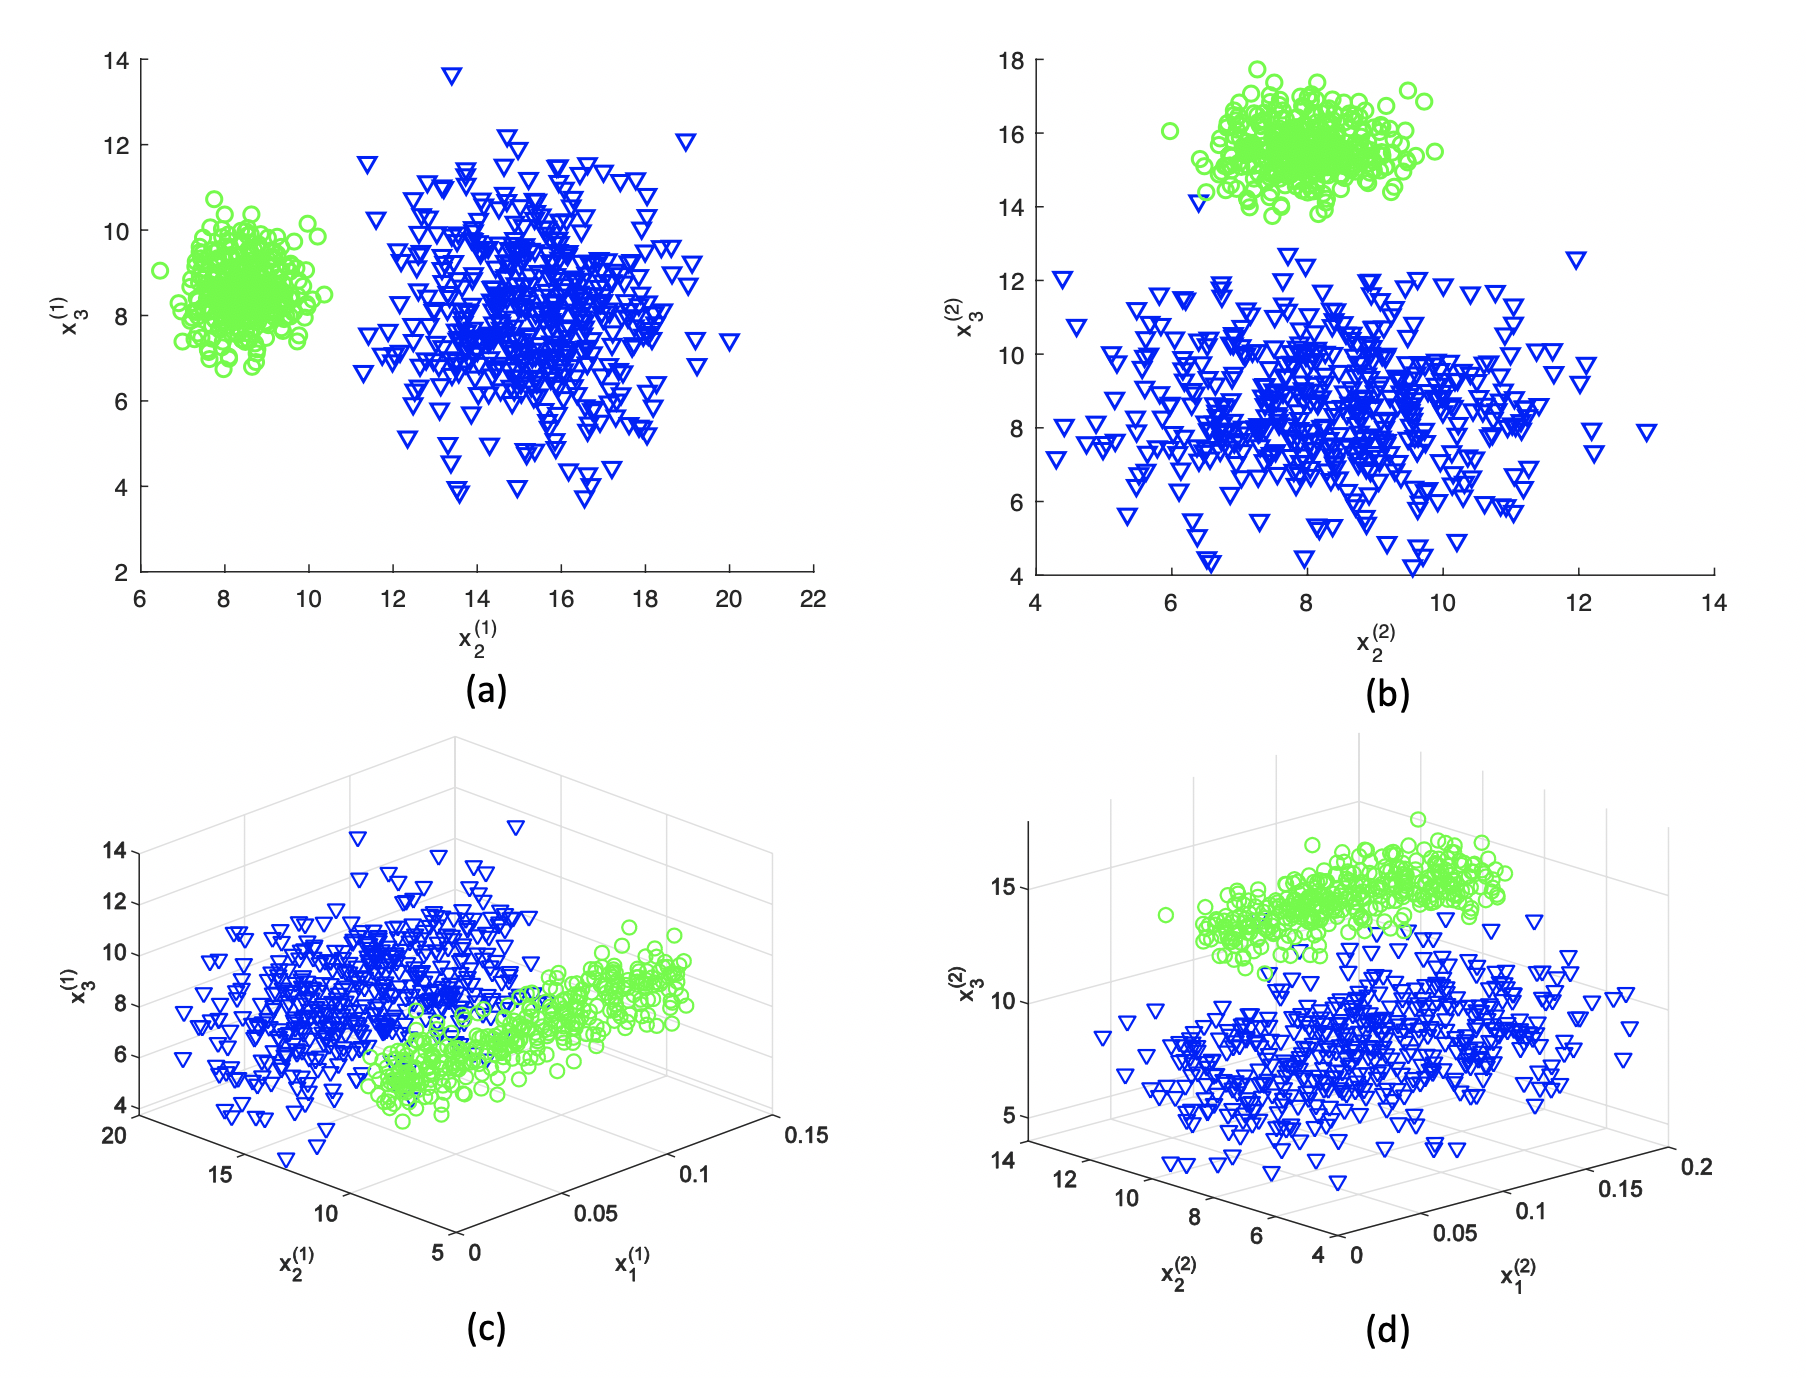
\includegraphics[width=1.2\textwidth]{2c2v.png}
     \end{center}
  \end{column}
  \begin{column}{0.7\textwidth}  %%<--- here
    \begin{itemize}
	  \item 55\% of the data points are in the blue group and 45\% in the green group
\item In view 2, the blue and the green ones are blended, which is it can end up to the wrong conclusion if the algorithms failed in getting the critical insight for structuring the data
	\end{itemize}
  \end{column}
\end{columns}


\end{frame}
%---------------------------------------------------------------------------------------------------------------------------


\begin{frame}{Another artificial example }
An artificial spherical-shape of a two-view numerical data set with 4 clusters and 2 feature components is considered. 

\begin{columns}
  \begin{column}{0.3\textwidth}
    \begin{center}
     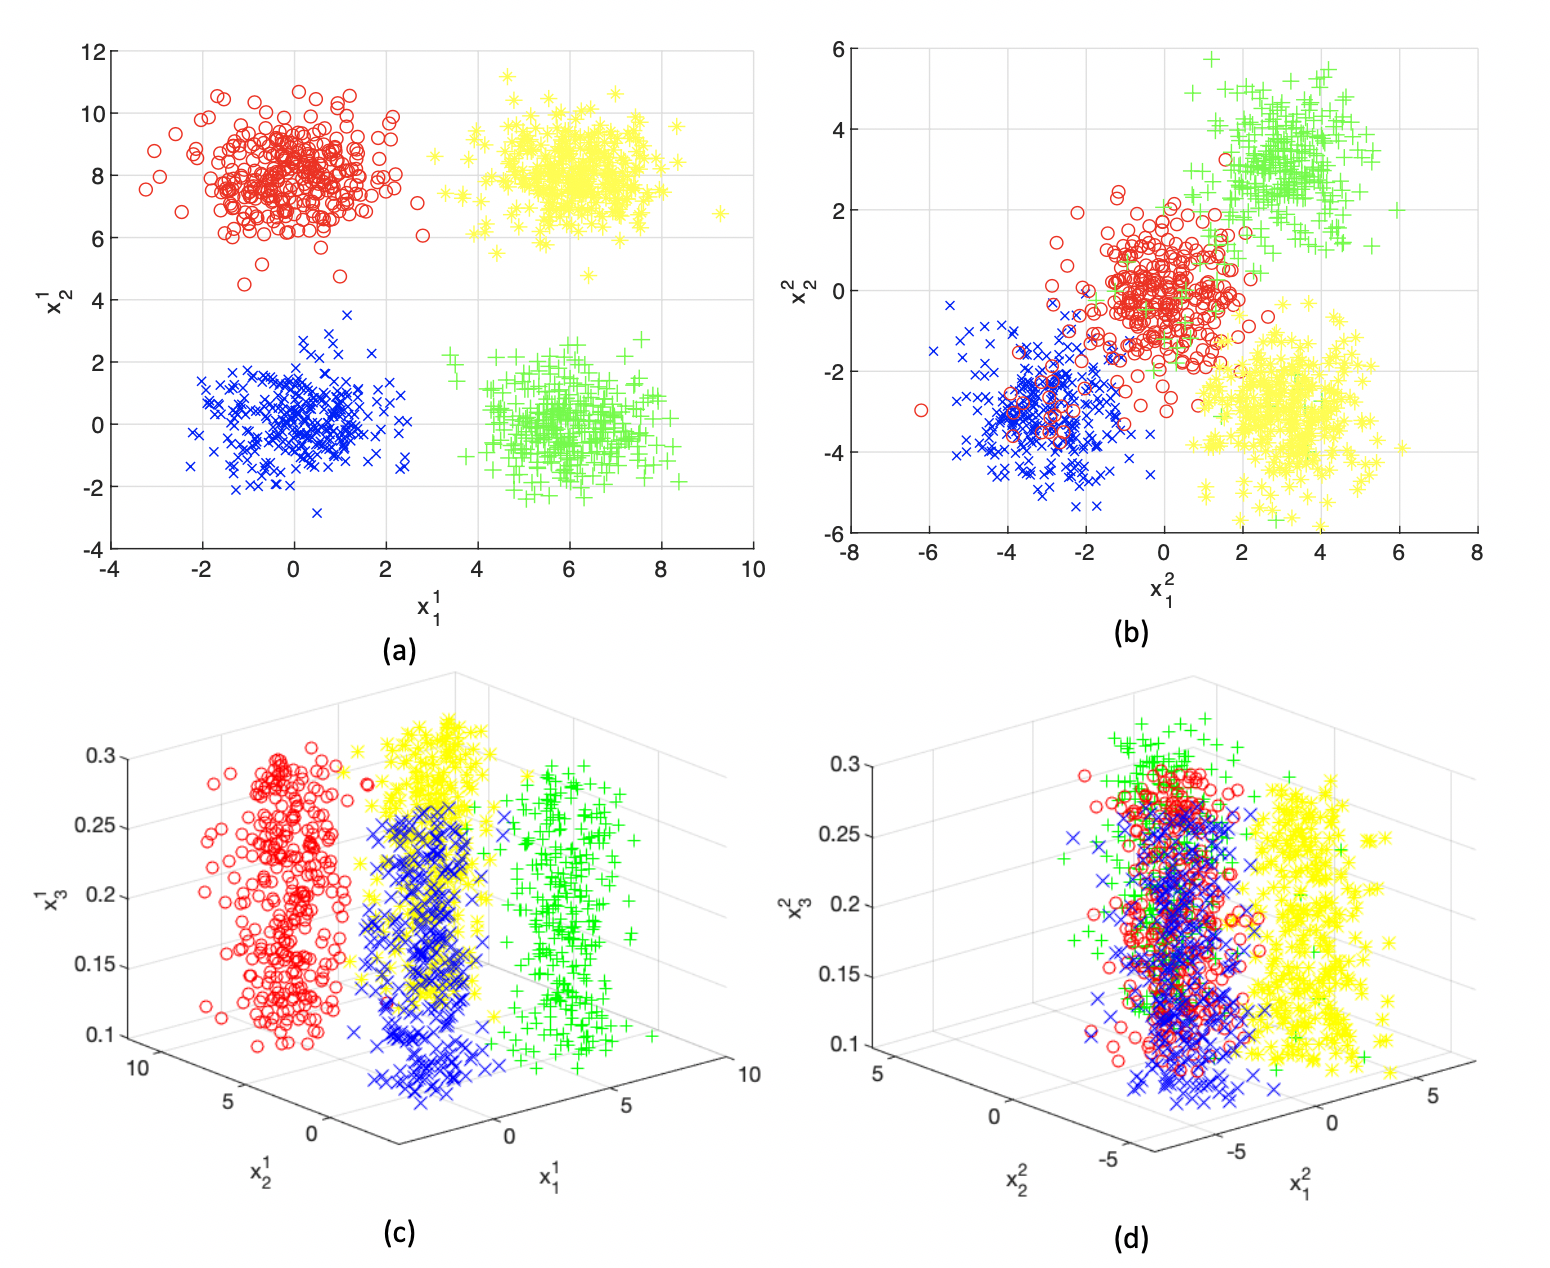
\includegraphics[width=1.2\textwidth]{4c2v.png}
     \end{center}
  \end{column}
  \begin{column}{0.7\textwidth}  %%<--- here
    \begin{itemize}
	  \item Another feature generated from a uniform distribution makes the data in (a)-(b) becomes severe
\item The presence of noise features in the data (a)-(b) makes the visual interpretation of a two-view numerical data set with 4 clusters chaos 
	\end{itemize}
  \end{column}
\end{columns}

\end{frame}

%---------------------------------------------------------------------------------------------------------------------------

\begin{frame}{Application: UCI Machine Learning Repository }

\begin{exampleblock}{Image Segmentation}
 The Image segmentation (IS) data set contains \alert{2310} instances of seven outdoor images. These \alert{seven} outdoor images are Brick-face, Sky, Foliage, Cement, Window, Path, and Grass. Each instance is represented by \alert{two} different views: \alert{9} features of the shape information and \alert{10} features of the RGB color \cite{27C.L.Blake1998UCISets}. 
\end{exampleblock}

\end{frame}

%---------------------------------------------------------------------------------------------------------------------------

\begin{frame}{Application: MSRC data set }
\vspace{-0.6cm}	

\begin{figure}
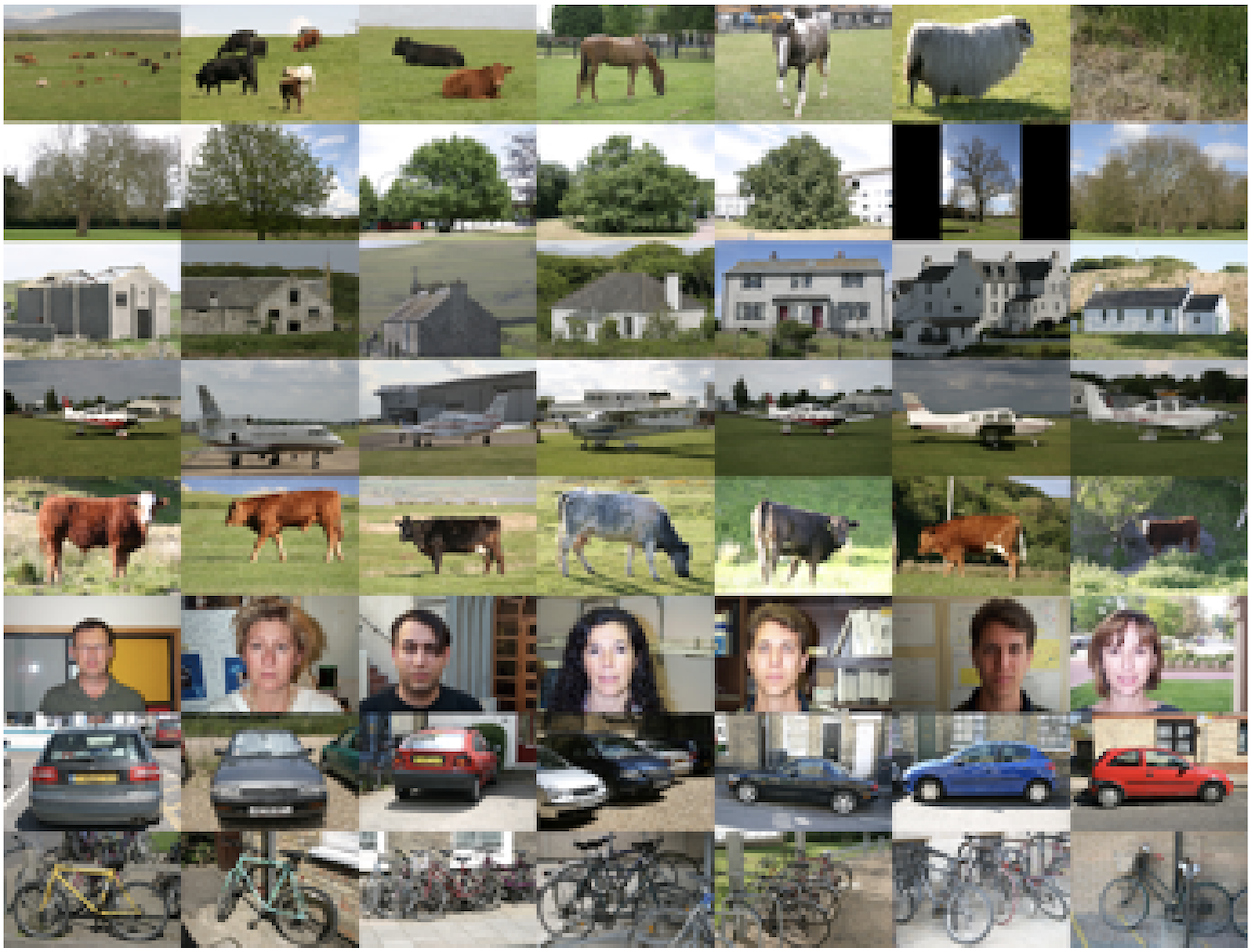
\includegraphics[width=7cm]{MSRC_V1.png}
  \caption{\label{fig:your-figure}Sample images from the MSRC-V1 data base.}
\end{figure}

\end{frame}
%---------------------------------------------------------------------------------------------------------------------------

\begin{frame}{Application: MSRC data set }

\begin{columns}
  \begin{column}{0.3\textwidth}
    \begin{center}
     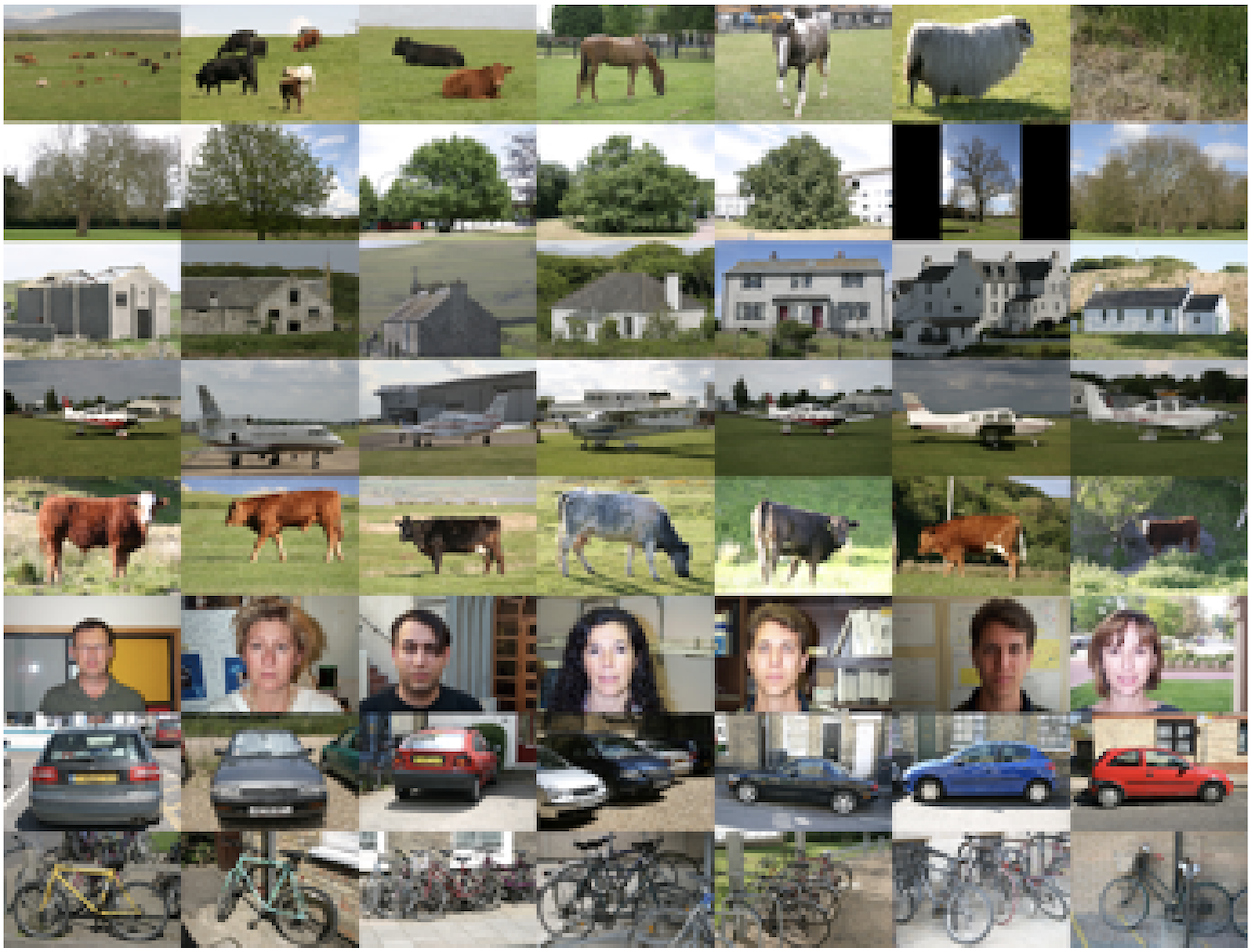
\includegraphics[width=1.2\textwidth]{MSRC_V1.png}
     \end{center}
  \end{column}
  \begin{column}{0.7\textwidth}  %%<--- here
    \begin{itemize}
	  \item The Microsoft Research Cambridge Volume 1 (MSRC-V1) data set has \alert{eight} classes, and each class has \alert{30} images \cite{Winn2005LOCUS:Segmentation}
	  \item We selected seven classes of eight classes with \alert{210} images in total
\item Each image is described by \alert{five} views (Color moment, CENTRIST, GIST, Histogram of oriented gradients (HOG), Local binary patterns (LBP))
	\end{itemize}
  \end{column}
\end{columns}

\end{frame}
%---------------------------------------------------------------------------------------------------------------------------



\begin{frame}{Application: Caltech-101 data set }

\begin{figure}
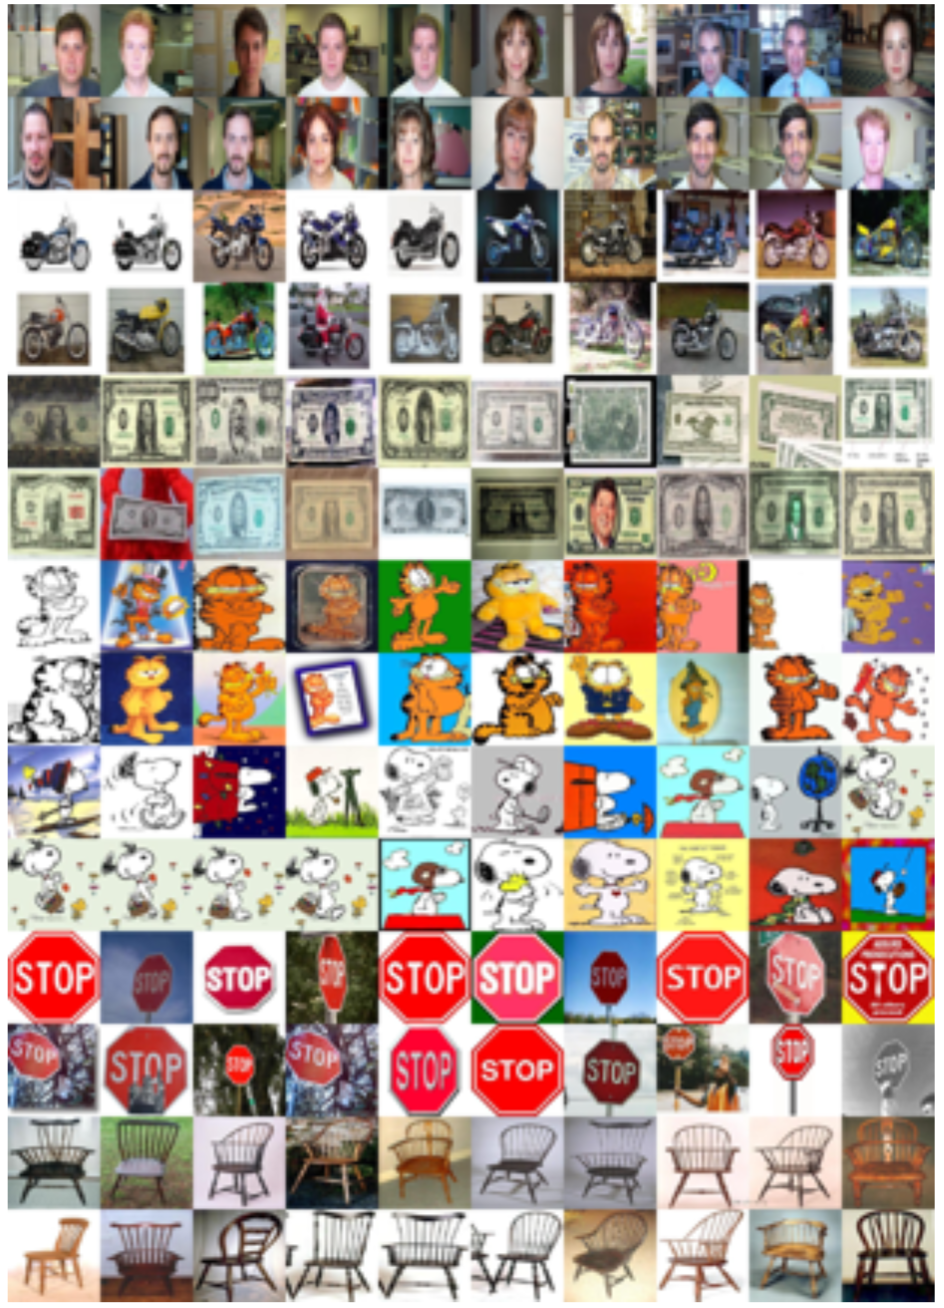
\includegraphics[width=5cm]{Caltech_sample.png}
\caption{\label{fig:your-figure} Sample images from the Caltech 101-7 data base}
\end{figure}

\end{frame}
%---------------------------------------------------------------------------------------------------------------------------

\begin{frame}{Application: Caltech-101 data set }

\begin{columns}
  \begin{column}{0.3\textwidth}
    \begin{center}
     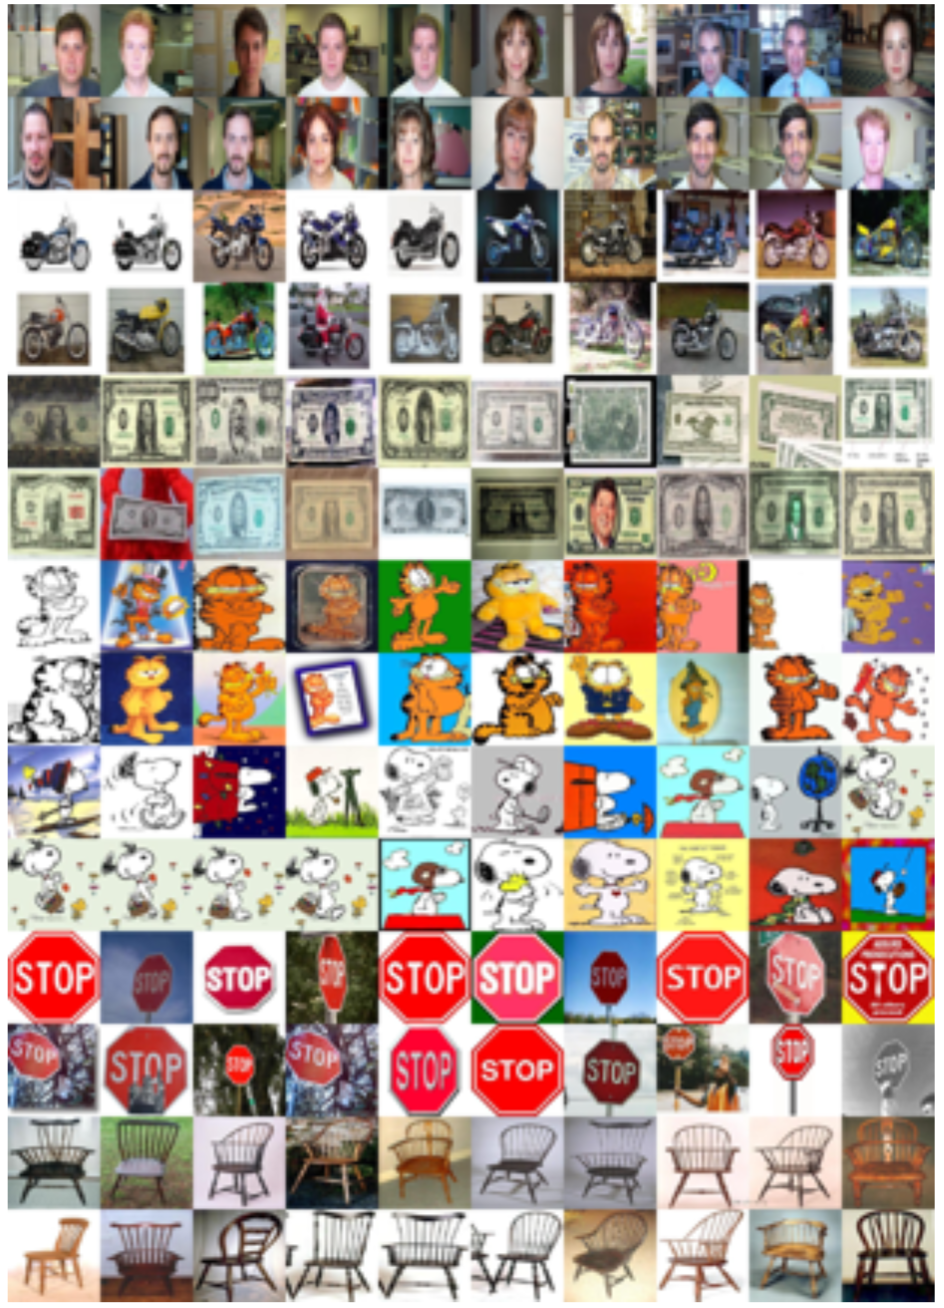
\includegraphics[width=1.2\textwidth]{Caltech_sample.png}
     \end{center}
  \end{column}
  \begin{column}{0.7\textwidth}  %%<--- here
    \begin{itemize}
	  \item Caltech 101 consists of a total of \alert{9.146} images belonging to \alert{101} categories \cite{Fei-Fei2007LearningCategories}
	  \item We selected \alert{seven} classes of 101 categories with \alert{1474} images in total
\item Each image is described by \alert{six} views (Gabor, CENTRIST, Histogram of oriented gradients (HOG), Wavelet moments, Local binary patterns (LBP), GIST)
	\end{itemize}
  \end{column}
\end{columns}

\end{frame}
%---------------------------------------------------------------------------------------------------------------------------

\begin{frame}{Application: Biological Data }

\begin{exampleblock}{Prokaryotic phyla }
 This biological data involved \alert{551} types of Prokaryotic species where each species described by \alert{three} views, including one textual data view and two genomic data views. The 2 genomic data views are known as gene repertoire and proteome composition \cite{Brbic2016TheGenes}. 
\end{exampleblock}


\end{frame}
%---------------------------------------------------------------------------------------------------------------------------

\begin{frame}{Text Data: UCI Machine Learning Repository}
\vspace{-0.6cm}	
Text recognition is the process of detecting text in images and video streams and recognizing the text contained therein. 

\begin{exampleblock}{Internet Advertisements }
 This data set represent a set of possible advertisements on internet pages. This data set consists of \alert{1559} columns and \alert{3279} number of instances in the data. Each instance in the data represents one image that is tagged as an advertisement (“ad”) and non-advertisement (“non-ad”) in the last column \cite{27C.L.Blake1998UCISets}. \\
 Each instance is described by \alert{six} different views (Geometry of the image, base URL, image URL, alt text, anchor text, target URL). 
\end{exampleblock}


\end{frame}
%---------------------------------------------------------------------------------------------------------------------------

\begin{frame}{Application: Multimedia data set }

\begin{figure}
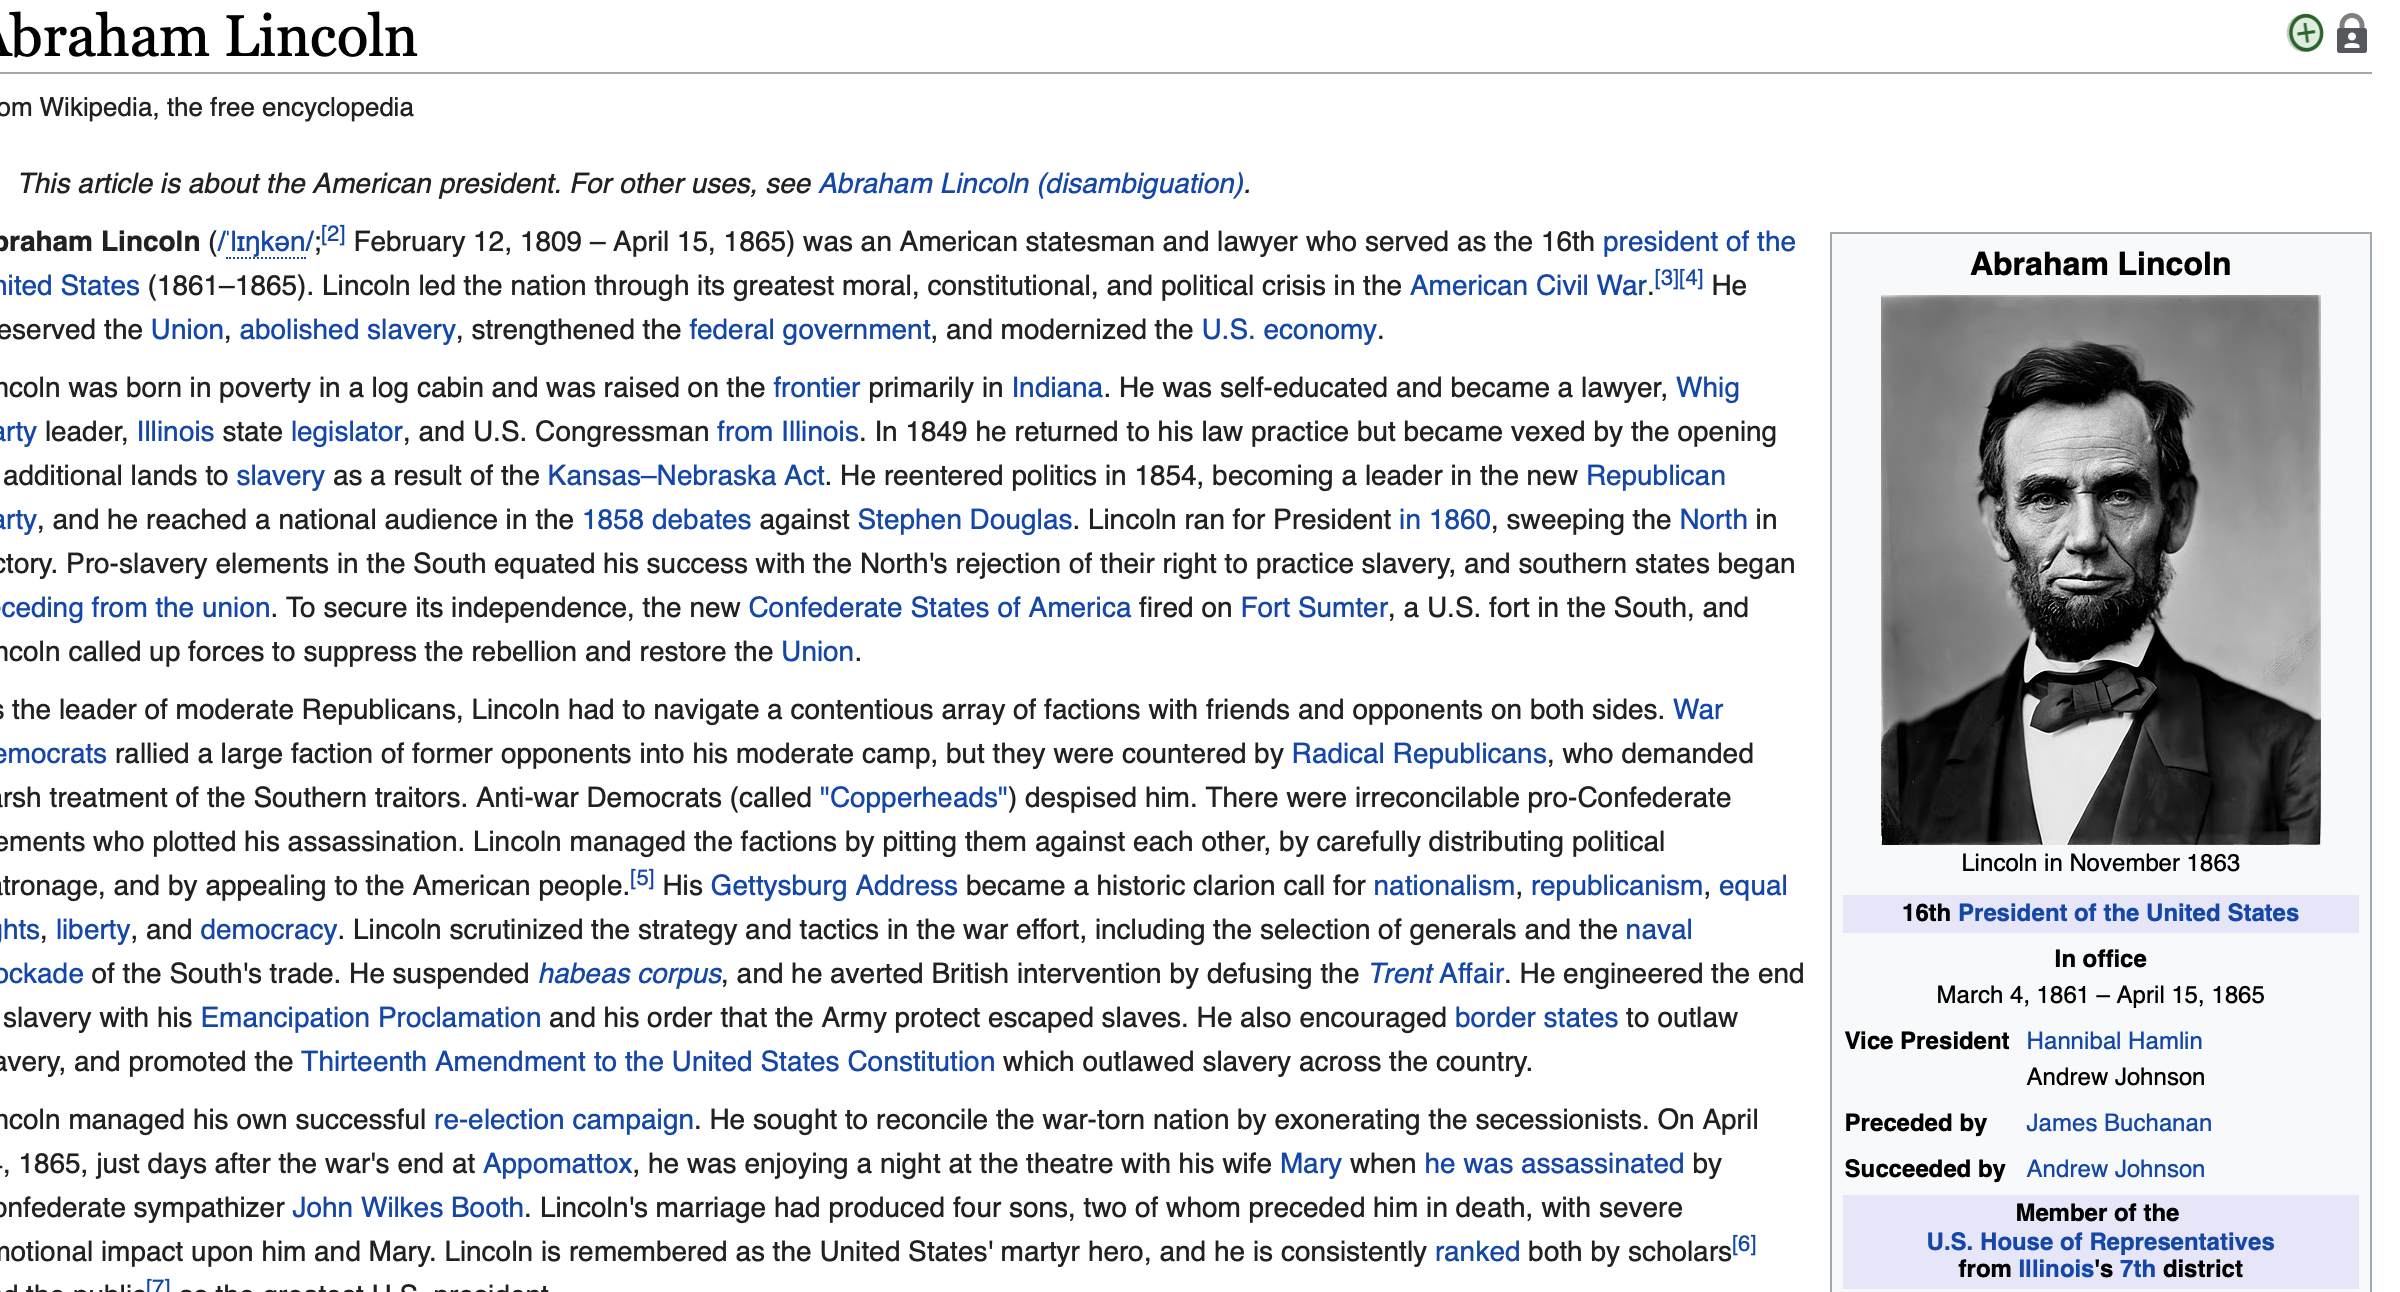
\includegraphics[width=7cm]{Abraham_Lin.png}
\caption{\label{fig:your-figure} Example of a combination of two data types such as text and images:  section from the Wikipedia article on the Abraham Lincoln}
\end{figure}

\end{frame}
%---------------------------------------------------------------------------------------------------------------------------

\begin{frame}{Application: Multimedia data set II}

\begin{figure}
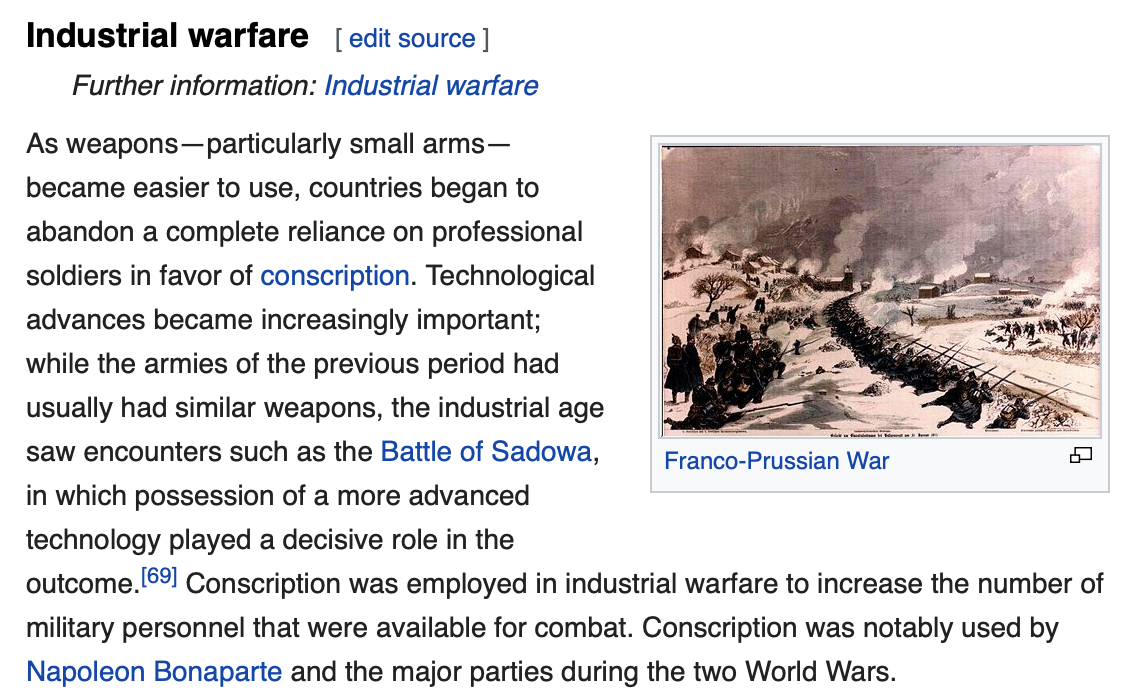
\includegraphics[width=7cm]{warfare.png}
\caption{\label{fig:your-figure} Example of a combination of two data types such as text and images:  part of a series 
on War history (Industrial warfare category).
}
\end{figure}

\end{frame}
%---------------------------------------------------------------------------------------------------------------------------

\begin{frame}{Wikipedia Articles: Figures results}

\begin{itemize}
\item The value of retrieval of some text and images gathers a wealth of historical information about Abraham Lincoln and Industrial warfare
\item The representation of information and knowledge becomes more explorable and understandable to the human users who need insights on specific topic
\end{itemize}

\end{frame}
%---------------------------------------------------------------------------------------------------------------------------


\begin{frame}{Multimedia: Wikipedia Articles}\begin{itemize}
\item Costa Pereira et al. retrieved \alert{2669} articles, and each article is assigned over \alert{29} categories, including the wiki text and image \cite{CostaPereira2014OnRetrieval}.
\item \alert{Ten} top-level categories are highlighted such as art & architecture, geography & places, history, literature & theatre, biology, media, music, sport & recreation, royalty & nobility, and warfare.
\item A random split was used to produce a training set of \alert{2173} documents and a test set of \alert{693} documents.
\end{itemize}

\end{frame}
%---------------------------------------------------------------------------------------------------------------------------

\begin{frame}{Data preparation process}

\begin{columns}
  \begin{column}{0.3\textwidth}
    \begin{center}
     {\Huge\calligra \textbf{WHEN} }
     \end{center}
     \begin{center}
     {\Huge\calligra \textbf{WHY} }
     \end{center}
     \begin{center}
     {\Huge\calligra \textbf{HOW} }
     \end{center}
  \end{column}
  \begin{column}{0.7\textwidth}  %%<--- here
       \begin{center}
     
\includegraphics[width=0.6\textwidth]{question-marks.jpg}
     \end{center}
  \end{column}
\end{columns}


\end{frame}
%---------------------------------------------------------------------------------------------------------------------------

\begin{frame}{Data preparation process: WHEN?}

The high dimensional data sets are often sparse, heterogeneous, uncertain, incomplete, missing, and derive.

\end{frame}
%---------------------------------------------------------------------------------------------------------------------------

\begin{frame}{Data preparation process: WHY?}

\begin{itemize}
\item There is a need for a unified and coherent machine learning framework that can analyze Big Data of different data characteristics and different application problem domains
\item Each machine learning models has different circumstances in discovering the structured of data
\item The accuracy of the algorithms is largely influenced by the type of data characteristics. 
\item To fix the failures of data clustering algorithms under different types of variations in the data
\end{itemize}


\end{frame}
%---------------------------------------------------------------------------------------------------------------------------

\begin{frame}{Data preparation process: HOW?}

\begin{enumerate}
\item Data cleaning
\item Data integration
\item Data transformation
\item Data reduction
\item Data discretization
\end{enumerate}


\end{frame}
%---------------------------------------------------------------------------------------------------------------------------


%%%%%%%%%%%%%%%%%%%%%%%%%%%%%%%%%%%%%%%%%%%%%%%
\section{Clustering Algorithms}
%%%%%%%%%%%%%%%%%%%%%%%%%%%%%%%%%%%%%%%%%%%%%%%

% =================================================================

\begin{frame}{}
    \centering
    \Huge{\textbf{Clustering Algorithms}}
\end{frame}
% =================================================================

\subsection{Single-view clustering}

\begin{frame}{K-means clustering}
	\vspace{-0.3cm}	

    
Objective function 

	\begin{equation}
            J(U, A)  = \sum_{i=1}^{n}\sum_{k=1} ^{c}\mu_{ik}\|x_{i}-a_{k}\|^2
            \label{updateU} % removed \\
        \end{equation}
Update equations

	\begin{equation}
            a_{k}  = \frac{\sum_{i=1}^{n}\mu_{ik} x_{ij}} {\sum_{i=1}^{n}\mu_{ik}}
            \label{updateA} % removed \\
        \end{equation} \begin{equation}\label{knuth1} \mu_{ik}=
\begin{cases}
1      &\text{if }\  \|x_{i}-a_{k}\|^2 = \min\limits_{1\leq k\leq c}\|x_{i}-a_{k}\|^2\\
0      & \text{Otherwise}
\end{cases}
\end{equation}
        

\end{frame}

%--------------------------------------------------------------------------------------------------------------------

\begin{frame}{Fuzzy c-means clustering}
	\vspace{-0.3cm}	
    
Objective function 

	\begin{equation}
            J_{FCM}(U, A)  = \sum_{i=1}^{n}\sum_{k=1} ^{c}\mu_{ik}^{m}\|x_{i}-a_{k}\|^2
            \label{updateU} % removed \\
        \end{equation}
Update equations

	\begin{equation}
            a_{k}  = \frac{\sum_{i=1}^{n}\mu_{ik}^{m}x_{ij}} {\sum_{i=1}^{n}\mu_{ik}^{m}}
            \label{updateA} % removed \\
        \end{equation}
        \begin{equation}
            \mu_{ik}  = \left ({\sum_{k’=1}^{c} ( d_{ik}/d_{ik'})^\frac{2} 
            {m-1}}\right)^{-1}   
            \label{updateU} % removed \\
        \end{equation}


\end{frame}


%--------------------------------------------------------------------------------------------------------------------

\subsection{Collaborative clustering}


\begin{frame}{Co-FC (Collaborative Fuzzy c-means clustering)}
	\vspace{-0.3cm}	
    
Objective function     
 \begin{equation}
\begin{aligned}
J_{Co-FC} \ (h)  ={} & \sum_{i=1}^{n}\sum_{k=1}^{c} \left(\mu_{ik}^{h} \right)^{m} \sum_{j=1}^{d_{h}} \left(x_{ij}^{h}-a_{kj}^{h}\right)^2  \\
      &   + \sum_{h'=1, h'\neq h}^{s} \alpha_{hh'} \sum_{i=1}^{n}\sum_{k=1}^{c}\left( \mu_{ik}^{h}-\mu_{ik}^{h'} \right )^{2}\sum_{j=1}^{d_{h}} \left(x_{ij}^{h}-a_{kj}^{h}\right)^2
\end{aligned}
\label{CoFC1} 
\end{equation}
where $\alpha_{hh'}$ is a disagreement values between the $hth$ database and the $h’th$ database \cite{Pedrycz2002CollaborativeClustering}. 

\end{frame}


%--------------------------------------------------------------------------------------------------------------------

\begin{frame}{Co-FC: Limitations}
	\vspace{-0.3cm}	
    
\begin{itemize}
\item This technique does not applicable for multi-sources data 
\item It does not clear how to estimate an appropriate values of $\alpha_{hh'}$ such as different data plays different roles of $\alpha_{hh'}$ .
\end{itemize}


\end{frame}


%--------------------------------------------------------------------------------------------------------------------

\begin{frame}{Co-FKM: Objective function}
	\vspace{-0.3cm}	
Objective function \cite{Cleuziou2009CoFKM:Clustering}     
\begin{equation}
J_{Co-FKM}   = \sum_{h=1}^{s} \sum_{i=1}^{n}\sum_{k=1}^{c} \left(\mu_{ik}^{h} \right)^{m} \sum_{j=1}^{d_{h}} \left(x_{ij}^{h}-a_{kj}^{h}\right)^2+\eta\Delta
\label{Co-FKM} 
\end{equation}
where \begin{equation*}
\Delta=\frac{1}{s-1}\sum_{h'=1, h'\neq h}^{s}\sum_{i=1}^{n}\sum_{k=1}^{c}\bigg\{ \left(\mu_{ik}^{h'}\right)^{m}-\left(\mu_{ik}^{h}\right)^{m} \bigg\}\sum_{j=1}^{d_{h}} \left(x_{ij}^{h}-a_{kj}^{h}\right)^2
\label{Delta} 
\end{equation*} 

\end{frame}


%--------------------------------------------------------------------------------------------------------------------

\begin{frame}{Co-FKM: Limitations}
	\vspace{-0.3cm}	
    
\begin{itemize}
\item Treated the importance of each view equally
\item Parameter $\eta$ is sensitive and user define
\item The fuzzier parameter $m$ is sensitive
\end{itemize}

\end{frame}


%--------------------------------------------------------------------------------------------------------------------

%--------------------------------------------------------------------------------------------------------------------

\begin{frame}{WV-Co-FCM: Objective function}
	\vspace{-0.3cm}	
Objective function \cite{Jiang2015CollaborativeViews}    
\begin{equation}
J_{WV-Co-FCM}   = \sum_{h=1}^{s}v_{h} \left( J_{FCM}^{h} + \Delta_{h} \right)+\beta\sum_{h=1}^{s} v_{h} \ \text{ln} \ v_{h}
\label{Co-FKM} 
\end{equation}
where \begin{equation*}
J_{FCM}^{h}=\sum_{i=1}^{n}\sum_{k=1}^{c} \left(\mu_{ik}^{h} \right)^{m} \sum_{j=1}^{d_{h}} \left(x_{ij}^{h}-a_{kj}^{h}\right)^2
\label{Delta} 
\end{equation*} 

\end{frame}


%--------------------------------------------------------------------------------------------------------------------

\begin{frame}{WV-Co-FCM: Short Explanation}
	\vspace{-0.3cm}	    
\begin{equation*}
\Delta_{h}   = \sum_{i=1}^{n} \alpha_{ik}^{h} \sum_{k=1}^{c} \mu_{ik}^{h} \Big ( 1- \left( \mu_{ik}^{h} \right )^{m-1} \Big ) - \sum_{i=1}^{n}\delta_{ik}^{h} \sum_{k=1}^{c} \mu_{ik}^{h} \Big ( 1- \left( \mu_{ik}^{h} \right )^{m-1} \Big )
\label{Delta1} 
\end{equation*}
\begin{columns}[c] % The "c" option specifies centered vertical alignment while the "t" option is used for top vertical alignment

\column{.6\textwidth} % Left column and width
\textbf{$\mathbf{\delta_{ik}^{h}}$ has four cases}
\begin{equation*}
\begin{aligned}
{} & \scriptstyle\text{Case 1: }\eta \frac{1}{s-1}\sum_{h'=1, h'\neq h}^{s}\sum_{j=1}^{d_{h'}}\left(x_{ij}^{h'}-a_{kj}^{h'}\right)^2\\
      & \scriptstyle \text{Case 2: } \frac{\eta}{s}\sum_{h=1}^{s}\sum_{j=1}^{d_{h}}\left(x_{ij}^{h}-a_{kj}^{h}\right)^2\\
      & \scriptstyle \text{Case 3: } \eta \min\limits_{h'\neq h}\big\{ \sum_{j=1}^{d_{h'}} \left ( x_{ij}^{h'}-a_{kj}^{h'} \right )^{2} \big \} \\
      & \scriptstyle \text{Case 4}: \eta \sqrt[s-1]{\prod_{h'\neq h} \sum_{j=1}^{d_{h'}} \left ( x_{ij}^{h'}-a_{kj}^{h'} \right )^{2} }
\end{aligned}
\label{constraint1}
\end{equation*}
\column{.4\textwidth} % Right column and width
\textbf{While }\begin{equation*}
\alpha_{ik}^{h} = \eta \sum_{j=1}^{d_{h}}\left(x_{ij}^{h}-a_{kj}^{h}\right)^2
\label{alpha1} 
\end{equation*}

\end{columns}

\end{frame}


%--------------------------------------------------------------------------------------------------------------------


\begin{frame}{WV-Co-FCM: Limitations}
	\vspace{-0.3cm}	
    
\begin{itemize}
\item Treated the importance of feature-view equally
\item Parameter $\beta$ and $\eta$ are sensitive 
\item The fuzzier parameter $m$ is sensitive
\end{itemize}

\end{frame}


%--------------------------------------------------------------------------------------------------------------------


\begin{frame}{Global Solutions: Co-FKM \& WV-Co-FCM}
	\vspace{-0.3cm}	    

\begin{itemize}
\item \textbf{Co-FKM}\begin{equation}
\tilde{\mu}_{ik} = \sqrt[s]{\prod_{h=1}^{s}  \mu_{ik}^{h}}
\label{SCoFKM} 
\end{equation}
\item \textbf{WV-Co-FCM }\begin{equation}
\tilde{U} =  \sum_{h=1}^{s} v_{h} U^{h}
\label{SWVCoFCM} 
\end{equation}

\end{itemize}



\end{frame}


%--------------------------------------------------------------------------------------------------------------------



\subsection{Minimax Optimization}

\begin{frame}{Minimax-FCM}
	\vspace{-0.3cm}	
    
    Objective function     
\begin{equation}
J_{\text{minimax-FCM}} \left (V, U^{*}, A^{h} \right ) = \sum_{h=1}^{s} \left (v_{h} \right )^{\beta} \sum_{i=1}^{n}\sum_{k=1}^{c} \left(\mu_{ik}^{*} \right)^{m} \sum_{j=1}^{d_{h}}\left(x_{ij}^{h}-a_{kj}^{h}\right)^2
\label{MinimaxFCM} 
\end{equation}
\vspace{-0.2cm}	
\\In the minimax-FCM, Wang and Chen \cite{Wang2017Multi-viewSources} used the min-max optimization with 
\begin{equation*}
\min\limits_{U^{*}, \{ A^{h}\}_{h=1}^{s}}   \max\limits_{ \{ v_{h}\}_{h=1}^{s}}   \sum_{h=1}^{s} \left (v_{h} \right )^{\beta} \sum_{i=1}^{n}\sum_{k=1}^{c} \left(\mu_{ik}^{*} \right)^{m} \sum_{j=1}^{d_{h}}\left(x_{ij}^{h}-a_{kj}^{h}\right)^2
\label{MinimaxFCM} 
\end{equation*}
\end{frame}


%--------------------------------------------------------------------------------------------------------------------

\begin{frame}{Minimax-FCM: Limitations}
	\vspace{-0.3cm}	
    
\begin{itemize}
\item Treated the importance of feature-view equally
\item Parameter $\beta$ is a user define
\item The fuzzier parameter $m$ is sensitive
\end{itemize}

\end{frame}


%--------------------------------------------------------------------------------------------------------------------

\subsection{Nonnegative Matrix Factorization}

\begin{frame}{MultiNMF: Objective Function}
	\vspace{-0.3cm}	
    
    Objective function     
\begin{equation}
J_{\text{MultiNMF}}  = \sum_{h=1}^{s} \Big \|X^{h}-U^{h} \left ( A^{h} \right )^{T} \Big \|_{F}^{2}  + \sum_{h=1}^{s} \lambda_{h} D \left( A^{h}, A^{*} \right )
\label{MinimaxFCM} 
\end{equation}
\begin{itemize}
\item Where $D \left( A^{h}, A^{*} \right) = \Big \| A^{h} - A^{*}\Big \|_{F}^{2}$  is the Frobenius norm and used as a measure of disagreement between the cluster indicator matrix  $A^{h}$ and the cluster consensus matrix $A^{*}$ of the $h$th view \cite{Liu2013Multi-viewFactorization}.
\end{itemize}



\end{frame}


%--------------------------------------------------------------------------------------------------------------------


\begin{frame}{MultiNMF: Limitations}
	\vspace{-0.3cm}	
    
\begin{itemize}
\item Treated the importance of each view equally
\item Treated the importance of feature-view equally
\item Parameter $\lambda_{h}$ is a user define and sensitive
\item Depends on normalization process because Input data must be in a positive value
\end{itemize}

\end{frame}


%--------------------------------------------------------------------------------------------------------------------


%%%%%%%%%%%%%%%%%%%%%%%%%%%%%%%%%%%%%%%%%%%%%%%
\section{The Proposed Algorithms}
%%%%%%%%%%%%%%%%%%%%%%%%%%%%%%%%%%%%%%%%%%%%%%%

% =================================================================

\begin{frame}{}
    \centering
    \Huge{\textbf{The Proposed Algorithms}}
\end{frame}
% =================================================================

% =================================================================

\begin{frame}{}
    \centering
\Huge{\textbf{Feature-weighted MVFCM (FW-MVFCM)}}
\end{frame}
% =================================================================

\subsection{FW-MVFCM }


\begin{frame}{FW-MVFCM: Introduction}
	\vspace{-0.3cm}	
   
   \begin{itemize}
   \item    The FW-MVFCM deal with multi-representated data 
\item The goal: Compute a similarity matrix for data object/point which appear in different views by considering the importance of each feature-view components.
\item The idea: create a simple feature weighting in multi-view FCM by incorporated the local membership of different views directly into a single global membership. 
   \end{itemize}
        

\end{frame}

%--------------------------------------------------------------------------------------------------------------------

\begin{frame}{FW-MVFCM: Objective function}
	\vspace{-0.3cm}	
    
        Objective function 

	\begin{equation}
          \scriptstyle  J_{FW-MVFCM}  = \sum_{h=1}^{s} (v_{h})^{\beta}\sum_{i=1}^{n}\sum_{k=1}^{c} \mu_{ik}^{m} \sum_{j=1}^{d_{h}} (w_j^{h})^2 \left(x_{ij}^{h}-a_{kj}^{h}\right)^2
            \label{MVFCM} % removed \\
        \end{equation}
\\Subject to
         \begin{equation}
\begin{aligned}
{} & \scriptstyle\sum_{k=1}^{c}\mu_{ik}=1, \mu_{ik}\in[0,1]\\
      & \scriptstyle\sum_{h=1}^{s}v_{h}=1, v_{h}\in[0,1]\\
      & \scriptstyle\sum_{j=1}^{d_h} w_j^{h}= 1, w_j^{h}\in[0,1].
\end{aligned}
\label{constraint1}
\end{equation}
        

\end{frame}

%--------------------------------------------------------------------------------------------------------------------


\begin{frame}{FW-MVFCM: Theorem 1}
	\vspace{-0.3cm}	
The updating equations for necessary conditions to minimize the $J_{FW-MVFCM}$  of Equations (\ref{MVFCM}) are 

\begin{align}
   &a_{kj}^{h}  = \frac{\sum_{i=1}^{n}\mu_{ik}^{m}x_{ij}^{h}} {\sum_{i=1}^{n}\mu_{ik}^{m}} \label{UpdatingA}  \\
  &v_{h}  =\left(\sum_{r=1}^{s}\left(\frac{\sum_{i=1}^{n}\sum_{k=1}^{c}  \mu_{ik}^{m} (w_j^{h})^2  \left(x_{ij}^{h}-a_{kj}^{h}\right)^2} {\sum_{i=1}^{n}\sum_{k=1}^{c}  \mu_{ik}^{m} (w_j^{r})^2  \left(x_{ij}^{r}-a_{kj}^{r}\right)^2} \right)^\frac{1}{\beta-1} \right)^{-1}
  \label{UpdatingV} 
\end{align}
\end{frame}

%---------------------------------------------------------------------------------------------------------------------------


\begin{frame}{FW-MVFCM: Theorem 1 Part II}
	\vspace{-0.3cm}	

	
	\begin{align}
     &w_{j}^{h}  =\sum_{j’=1}^{d_{h}}\left(\frac{\left(v_{h}\right)^{\beta}\sum_{i=1}^{n}\sum_{k=1}^{c}  \mu_{ik}^{m}   \left(x_{ij}^{h}-a_{kj}^{h}\right)^2} {\left(v_{h}\right)^{\beta}\sum_{i=1}^{n}\sum_{k=1}^{c}  \mu_{ik}^{m}  \left(x_{ij’}^{h}-a_{kj’}^{h}\right)^2} \right)^{-1} \label{UpdatingW} \\
	&\mu_{ik}  =\left(\left(\sum_{l=1}^{c} \frac{\sum_{h=1}^{s}\left(v_{h}\right)^{\beta} \sum_{j=1}^{d_{h}}(w_j^{h})^2  \left(x_{ij}^{h}-a_{kj}^{h}\right)^2} {\sum_{h=1}^{s}\left(v_{h}\right)^{\beta}\sum_{j=1}^{d_{h}}(w_j^{h})^2  \left(x_{ij}^{h}-a_{lj}^{h}\right)^2} \right)^\left(\frac{1}{m-1}\right) \right)^{-1}
    \label{UpdatingU} 
	\end{align}

	
\end{frame}
%----------------------------------------------------------------------------------------------------------------


\begin{frame}{FW-MVFCM: Proof $\mu_{ik}$}
	\vspace{-0.3cm}	
    
    We prove it by using Langrange multipliers. The Lagrangian of $J_{FW-MVFCM}$ subject to $\sum_{k=1}^{c}\mu_{ik}=1, \mu_{ik}\in[0,1] $ is $\hat{J}=J_{FW-MVFCM}-\lambda_{1} \left(\sum_{k=1}^{c}\mu_{ik}-1 \right)$
  \begin{align}
& \frac{\partial \tilde{J}}{\partial\mu_{ik}}=m\mu_{ik}^{m-1}\sum_{h=1}^{s}\left(v_{h}\right)^{\beta}\sum_{j=1}^{d_{h}} (w_j^{h})^2 \left(x_{ij}^{h}-a_{kj}^{h}\right)^2 - \lambda_{1}=0\\
& \mu_{ik}=\left(\frac{\lambda_{1}}{\sum_{h=1}^{s}\left(v_{h}\right)^{\beta}\sum_{j=1}^{d_{h}} (w_j^{h})^2 \left(x_{ij}^{h}-a_{kj}^{h}\right)^2 }\right)^\frac{1}{m-1}
\end{align}
	
\end{frame}
%---------------------------------------------------------------------------------------------------------------------------

\begin{frame}{FW-MVFCM: Proof $\mu_{ik}$}
	\vspace{-0.3cm}	
    \begin{itemize}
    
    \item Since $\sum_{l=1}^{c}\mu_{il}=1 $ we get
  \begin{equation}
\lambda_{1}=\frac{1}{\sum_{l=1}^{c}\left(\frac{1}{\sum_{h=1}^{s}\left(v_{h}\right)^{\beta}\sum_{j=1}^{d_{h}} (w_j^{h})^2 \left(x_{ij}^{h}-a_{lj}^{h}\right)^2 }\right)^\frac{1}{m-1}}
\end{equation}
\item Thus, the updating equation for $\mu_{ik}$ can be obtained as Equation (\ref{UpdatingU})  
	\end{itemize}
\end{frame}
%---------------------------------------------------------------------------------------------------------------------------

\begin{frame}{FW-MVFCM: Proof $v_{h}$}
	\vspace{-0.3cm}	
    \begin{itemize}
    
    \item We consider the Lagrangian of  (\ref{MVFCM}) subject to $\sum_{h=1}^{s}v_{h}=1 $ with  $\hat{J}=J_{FW-MVFCM}-\lambda_{2} \left(\sum_{h=1}^{s}v_{h}-1 \right)$
  \begin{align}
&\scriptstyle \frac{\partial \tilde{J}}{\partial v_{h}}=\beta \left(v_{h}\right)^{\beta-1}\left(\sum_{i=1}^{n}\sum_{k=1}^{c}  \mu_{ik}^{m} \sum_{j=1}^{d_{h}} (w_j^{h})^2  \left(x_{ij}^{h}-a_{kj}^{h}\right)^2\right)-\lambda_{2}=0\\
& v_{h}=\left(\lambda_{2}\right)^\frac{1}{\beta-1}\left(\sum_{i=1}^{n}\sum_{k=1}^{c}  \mu_{ik}^{m} \sum_{j=1}^{d_{h}} (w_j^{h})^2  \left(x_{ij}^{h}-a_{kj}^{h}\right)^2\right)^\frac{-1}{\beta-1}
\end{align}
	\end{itemize}
\end{frame}
%---------------------------------------------------------------------------------------------------------------------------

\begin{frame}{FW-MVFCM: Proof $v_{h}$}
	\vspace{-0.3cm}	
    \begin{itemize}
    
    \item Since $\sum_{r=1}^{s}v_{r}=1 $ we get
  \begin{equation}
\scriptstyle\left(\lambda_{2}\right)^\frac{1}{\beta-1}=\left(\sum_{r=1}^{s}\left(\sum_{i=1}^{n}\sum_{k=1}^{c}  \mu_{ik}^{m} \sum_{j=1}^{d_{r}} (w_j^{r})^2  \left(x_{ij}^{r}-a_{kj}^{r}\right)^2\right)^\frac{-1}{\beta-1}\right)^{-1}
\end{equation}
\item Thus, the updating equation for $v_{h}$ can be obtained as Equation (\ref{UpdatingV})  
	\end{itemize}
\end{frame}
%---------------------------------------------------------------------------------------------------------------------------


\begin{frame}{FW-MVFCM: Proof $w_{j}^{h}$}
	\vspace{-0.3cm}	
    \begin{itemize}
    
    \item We finally consider the Lagrangian of  (\ref{MVFCM}) subject to $\sum_{j=1}^{d_{h}}w_{j}^{h}=1 $ with  $\hat{J}=J_{FW-MVFCM}-\lambda_{3} \left(\sum_{j=1}^{d_{h}}w_{j}^{h}-1\right)$
    \begin{align}
& \frac{\partial \tilde{J}}{\partial w_{j}^{h}}=\left(v_{h}\right)^\beta\left(2\sum_{i=1}^{n}\sum_{k=1}^{c}  \mu_{ik}^{m} w_{j}^{h}  \left(x_{ij}^{h}-a_{kj}^{h}\right)^2\right)-\lambda_{3}=0\\
& w_{j}^{h}=\lambda_{3}\left(\left(v_{h}\right)^\beta\left(\sum_{i=1}^{n}\sum_{k=1}^{c}  \mu_{ik}^{m}  \left(x_{ij}^{h}-a_{kj}^{h}\right)^2\right)\right)^{-1}
\end{align}
	\end{itemize}
\end{frame}
%---------------------------------------------------------------------------------------------------------------------------

\begin{frame}{FW-MVFCM: Proof $w_{j}^{h}$}
	\vspace{-0.3cm}	
    \begin{itemize}
    
    \item Since $\sum_{j'=1}^{d_{h}}w_{j'}^{h}=1 $ we get
  \begin{equation}
\lambda_{3}=\left(\sum_{j'=1}^{d_{h}}\left(\left(v_{h}\right)^{\beta}\left(\sum_{i=1}^{n}\sum_{k=1}^{c}  \mu_{ik}^{m}  \left(x_{ij'}^{h}-a_{kj'}^{h}\right)^2\right)\right)^{-1}\right)^{-1}
\end{equation}
\item Thus, the updating equation for $w_{j}^{h}$ can be obtained as Equation (\ref{UpdatingW})  
	\end{itemize}
\end{frame}
%---------------------------------------------------------------------------------------------------------------------------

\begin{frame}{How FW-MVFCM's Algorithm Works}
	\vspace{-0.3cm}	
So how does a FW-MVFCM Algorithm work, I will explain this using six simple steps:
\begin{description}
\item [Input]
Data set $\boldsymbol{X}=\{ x_{1},. . .,x_{n} \}$ with $x_{i}^{h}=\{ x_{ij}^{h} \}_{j=1}^{d_{h}}$, number $c$ of cluster, $\beta=0$, and $\varepsilon>0$
\item[Output]
$w_{j}^{h}, v_{h}, a_{kj}^{h}, \mu_{ik}.$
\item[Initialization]
Randomly generate initial $U$, initialize feature weight $W^{h^{t}}=[w_{j}^{h}]_{1\times d_{h}}$ (user may define $w_{j}^{h}=1/d_{h}\forall j$), initialize view weight $V^{t}=[v_{h}]_{1\times s}$ (user may define $v_{h}=1/s\forall h$), and set $t=1.$
\item[Step 1]
Calculate $\beta$  by $\beta=t/n.$
\end{description}
\end{frame}
%---------------------------------------------------------------------------------------------------------------------------

\begin{frame}{How FW-MVFCM's Algorithm Works}
	\vspace{-0.3cm}	
\begin{description}
\item[Step 2]
Udate the feature weight $W^{h^{t}}$ using $A^{h^{t-1}}, U^{t-1}$, and $V^{t-1}$ by Eq. (\ref{UpdatingW}) .
\item[Step 3]
Update the view weight $V^{h^{t}}$ using $A^{h^{t-1}}, U^{t-1}$, and $W^{h^{t}}$ by Eq. (\ref{UpdatingV}).
\item[Step 4]
Update the cluster centers  $A^{h^{t}}$ using $ U^{t-1}$ by Eq. (\ref{UpdatingA}).
\item[Step 5]
Update membership  $U^{t}$ using $W^{h^{t}}$and $A^{h^{t}}$  by Eq. (\ref{UpdatingU}).
\item[Step 6]
If  $\left(\Big|\|U^{t}\|-\|U^{t-1}\|\Big|\right)\Big/nc<\varepsilon$ , then stop;
\item 
Else set $t=t+1$  and go back to Step 1.
\end{description}
\end{frame}
%---------------------------------------------------------------------------------------------------------------------


% =================================================================
\begin{frame}{}
    \centering
    \Huge{\textbf{From FW-MVFCM to Co-FW-MVFCM}}
\end{frame}
% =================================================================



%%%%%%%%%%%%%%%%%%%%%%%%%%%%%%%%%%%%%%%%%%%%%%%

\subsection{From FW-MVFCM to Co-FW-MVFCM}

%%%%%%%%%%%%%%%%%%%%%%%%%%%%%%%%%%%%%%%%%%%%%%%
% Co-FW-MVFCM

\begin{frame}{Modification of FW-MVFCM: Introduction}
	\vspace{-0.3cm}	
   
   \begin{itemize}
   \item    The modification of FW-MVFCM's objective function is made to create the collaborative learning  within multi-representated data 
\item The idea: added the memberships of different views into the FW-MVFCM
   \end{itemize}
        

\end{frame}

%--------------------------------------------------------------------------------------------------------------------

\begin{frame}{Modification of FW-MVFCM: Objective Function}
	\vspace{-0.3cm}	
\scriptsize{Based on objective function of Eq. (\ref{MVFCM})}

	\begin{equation}
            J_{FW-MVFCM}  = \sum_{h=1}^{s} (v_{h})^{\beta}\sum_{i=1}^{n}\sum_{k=1}^{c} \left(\mu_{ik}^{h}\right)^{m} \sum_{j=1}^{d_{h}} (w_j^{h})^2 \left(x_{ij}^{h}-a_{kj}^{h}\right)^2
            \label{FW-MVFCM1} % removed \\
        \end{equation}Subject to
        
\begin{equation}
\begin{aligned}
{} & \sum_{k=1}^{c}\mu_{ik}^{h}=1, \mu_{ik}^{h}\in[0,1] \\
      & \sum_{h=1}^{s}v_{h}=1, v_{h}\in[0,1]\\
      & \sum_{j=1}^{d_h} w_j^{h}= 1, w_j^{h}\in[0,1].
\end{aligned}
\label{constraint}
\end{equation}
        


\end{frame}
%---------------------------------------------------------------------------------------------------------------------


% =================================================================

\begin{frame}{}
    \centering
    \Huge{\textbf{Collaborative FW-MVFCM (Co-FW-MVFCM)}}
\end{frame}

% =================================================================

%%%%%%%%%%%%%%%%%%%%%%%%%%%%%%%%%%%%%%%%%%%%%%%

\subsection{Co-FW-MVFCM}

%%%%%%%%%%%%%%%%%%%%%%%%%%%%%%%%%%%%%%%%%%%%%%%



\begin{frame}{Co-FW-MVFCM: Introdution}
	\vspace{-0.6cm}	

\begin{itemize}
\item \scriptsize Although we previously proposed the simplest one of feature-weighted MVFCM algorithms for clustering multi-view data. However, the correct classification rate is not enough that can be improved.
\item \scriptsize  This is because the recognition rate of the proposed feature-weighted MVFCM algorithm can evaluate the error of misclassification contained in the final partitioning, but it provides only partial information about the structural quality of the obtaining partition. 
\item \scriptsize That is, it may improve the clustering performance but the resulting partition might be practically useless. In order to get a more objective judgement about the partitioning quality, the exchanging information about the local partition between each view during the learning process should be taken into considerations. 
\end{itemize}


\end{frame}
%---------------------------------------------------------------------------------------------------------------------------

\begin{frame}{Co-FW-MVFCM: Objective Function}
	\vspace{-0.6cm}	
\scriptsize By referring to Equation (\ref{CoFC1}) of Pedrycz [17], we provide the collaborative learning into the objective function of Equation (\ref{FW-MVFCM1}) with 
    \begin{equation}
\begin{aligned}
J_{Co-FW-MVFCM}  ={} & \sum_{h=1}^{s} (v_{h})^{\beta}\sum_{i=1}^{n}\sum_{k=1}^{c} \left(\mu_{ik}^{h} \right)^{2}\left(d_{ik,w}^{h} \right)^2   \\
      & +\alpha \sum_{\substack{h'= 1\\ h'\ne h}}^{s}\sum_{i=1}^{n}\sum_{k=1}^{c}\{ \mu_{ik}^{h}-\mu_{ik}^{h'} \}^{2}\left(d_{ik,w}^{h} \right)^2
\end{aligned}
\label{Co-FW-MVFCM} 
\end{equation}
\item 
    \begin{equation}
\text{with} \ d_{ik,w}^{h}=\sqrt{\sum_{j=1}^{d_{h}}\left(w_{j}^{h}\right)^{2}\left(x_{ij}^{h}-a_{kj}^{h}\right)^{2}}
\label{d_ikw}
\end{equation}


\end{frame}
%---------------------------------------------------------------------------------------------------------------------------

\begin{frame}{Co-FW-MVFCM: Constraints}
	\vspace{-0.3cm}	
    \begin{itemize}
    Subject to
\begin{equation}
\begin{aligned}
{} & \sum_{k=1}^{c}\mu_{ik}^{h}=1, \mu_{ik}^{h}\in[0,1] \\
      & \sum_{h=1}^{s}v_{h}=1, v_{h}\in[0,1]\\
      & \sum_{j=1}^{d_h} w_j^{h}= 1, w_j^{h}\in[0,1].
\end{aligned}
\label{constraint1}
\end{equation}
    
	\end{itemize}

\end{frame}
%---------------------------------------------------------------------------------------------------------------------------


\begin{frame}{Co-FW-MVFCM: Highlighted Terminology }
\vspace{-0.7cm}
\begin{block}{Highlighted 1}
The first terms of Eq. (\ref{Co-FW-MVFCM}) is a single view partition process to produce a local clustering partition in each view.
\end{block}

\begin{exampleblock}{Highlighted 2}
The second terms of Eq. (\ref{Co-FW-MVFCM}) corresponds to the collaborative learning between views in multi-view data. 
\end{exampleblock}

\begin{alertblock}{Highlighted 3}
$m=2$ is a new regulation to optimize the parameters of the second terms of Eq. (\ref{Co-FW-MVFCM}). 
\end{alertblock}

\end{frame}
%---------------------------------------------------------------------------------------------------------------------

\begin{frame}{Global Solutions: Co-FW-MVFCM}
	   
In order to merge the partition matrices in each view and obtain the global clustering result, we adopt the summation of each weighted fuzzy partition matrix for each view as: 
\begin{equation}
\tilde{U} =  \sum_{h=1}^{s} v_{h} U^{h}
\label{GlobalCo} 
\end{equation}

\end{frame}


%--------------------------------------------------------------------------------------------------------------------


\begin{frame}{Co-FW-MVFCM: Theorem 2}
The updating equations for necessary conditions to minimize the $J_{Co-FW-MVFCM}$  of Equation (\ref{Co-FW-MVFCM}) are 

\begin{align}
   & \mu_{ik}^{h}=\bigg(1-\sum_{l=1}^{c}\Big(\frac{\varphi_{il}^{h}} {1+\alpha} \Big) \bigg)  \Bigg(\sum_{l=1}^{c} \frac {(d_{ik,w}^{h})^{2}} {(d_{il,w}^{h} )^{2}} \Bigg)^{-1} + \frac{\varphi_{ik}^{h}}{1+\alpha}  
  \label{Theorem2U} 
\end{align}

\end{frame}
%---------------------------------------------------------------------------------------------------------------------------

\begin{frame}{Co-FW-MVFCM: Theorem 2 Part II}

\begin{equation}
\begin{aligned}
v_{h}  ={} &  \Bigg ( \sum_{r=1}^{s} \bigg ( \frac { \sum_{i=1}^{n}\sum_{k=1}^{c} (\mu_{ik}^{h})^{2} (d_{ik,w}^{h})^{2} }  {\sum_{i=1}^{n}\sum_{k=1}^{c} (\mu_{ik}^{r})^{2} (d_{ik,w}^{r})^{2} }\\
      &  + \frac{\alpha \sum_{\substack{h'= 1\\ h'\ne h}}^{s} \sum_{i=1}^{n}\sum_{k=1}^{c}\{ \mu_{ik}^{h}-\mu_{ik}^{h'} \}^{2}(d_{ik,w}^{h})^{2} }  {\alpha \sum_{\substack{h'= 1\\ h'\ne r}}^{s}\sum_{i=1}^{n}\sum_{k=1}^{c}\{ \mu_{ik}^{r}-\mu_{ik}^{h'} \}^{2}(d_{ik,w}^{r})^{2}  \big )}  \bigg ) ^\frac{1}{\beta-1}\Bigg )^{-1}
\end{aligned}
\label{Theorem2V} 
\end{equation}

\end{frame}
%---------------------------------------------------------------------------------------------------------------------------

\begin{frame}{Co-FW-MVFCM: Theorem 2 Part III}

\begin{equation}
\begin{aligned}
w_{j}^{h}  ={} & \Bigg ( \sum_{j’=1}^{d_{h}} \bigg ( \frac { (v_{h})^{\beta} \big ( \sum_{i=1}^{n}\sum_{k=1}^{c}(\mu_{ik}^{h})^{2}(x_{ij}^{h}-a_{kj}^{h})^{2}}  {(v_{h})^{\beta} \big ( \sum_{i=1}^{n}\sum_{k=1}^{c}(\mu_{ik}^{h})^{2}(x_{ij’}^{h}-a_{kj’}^{h})^{2} } \\
      &  + \frac {\alpha \sum_{\substack{h'= 1\\ h'\ne h}}^{s}\sum_{i=1}^{n}\sum_{k=1}^{c}\{ \mu_{ik}^{h}-\mu_{ik}^{h'} \}^{2} (x_{ij}^{h}-a_{kj}^{h})^{2}  \big ) } {\alpha  \sum_{\substack{h'= 1\\ h'\ne h}}^{s}\sum_{i=1}^{n}\sum_{k=1}^{c}\{ \mu_{ik}^{h}-\mu_{ik}^{h'} \}^{2} (x_{ij’}^{h}-a_{kj’}^{h})^{2}  \big )}  \bigg ) \Bigg )^{-1}
\end{aligned}
\label{Theorem2W} 
\end{equation}

\end{frame}
%---------------------------------------------------------------------------------------------------------------------------


\begin{frame}{Co-FW-MVFCM: Theorem 2 Part IV}

\begin{equation}
\begin{aligned}
a_{kj}^{h}  ={} &  \frac { (v_{h})^{\beta}\sum_{i=1}^{n}(\mu_{ik}^{h})^{2} (w_{j}^{h})^{2} x_{ij}^{h}}  { (v_{h})^{\beta}\sum_{i=1}^{n}(\mu_{ik}^{h})^{2} (w_{j}^{h})^{2} } \\
      & +  \frac {\alpha \sum_{\substack{h'= 1\\ h'\ne h}}^{s} (v_{h})^{\beta} \sum_{i=1}^{n} \{ \mu_{ik}^{h}-\mu_{ik}^{h'} \}^{2} (w_{j}^{h})^{2} x_{ij}^{h}  } { \alpha \sum_{\substack{h'= 1\\ h'\ne h}}^{s} (v_{h})^{\beta} \sum_{i=1}^{n} \{ \mu_{ik}^{h}-\mu_{ik}^{h'} \}^{2} (w_{j}^{h})^{2} }
\end{aligned}
\label{Theorem2A} 
\end{equation}



\end{frame}
%---------------------------------------------------------------------------------------------------------------------------


\begin{frame}{Co-FW-MVFCM: Shortened Proof}
\vspace{-0.6cm}
Shortened Proof:
\begin{block}{Membership $\mu_{ik}^{h}$}
\begin{equation*}
\mu_{ik}^{h}=\bigg(1-\sum_{l=1}^{c}\Big(\frac{\varphi_{il}^{h}} {1+\alpha} \Big) \bigg)  \Bigg(\sum_{l=1}^{c} \frac {(d_{ik,w}^{h})^{2}} {(d_{il,w}^{h} )^{2}} \Bigg)^{-1} + \frac{\varphi_{ik}^{h}}{1+\alpha} 
   \label{UpdatingU1}  
\end{equation*}\\
\medskip
\end{block}
\underline{Proof} (by Langrangian multipliers): The Lagrangian of $J_{Co-FW-MVFCM}$  subject to $\sum_{k=1}^{c}\mu_{ik}^{h}=1, \mu_{ik}^{h}\in[0,1] $ is $\hat{J}=J_{Co-FW-MVFCM}-\lambda_{1} \left(\sum_{k=1}^{c}\mu_{ik}^{h}-1 \right)$


\end{frame}

%---------------------------------------------------------------------------------------------------------------------------

\begin{frame}{Co-FW-MVFCM: Shortened Proof}
By taking the partial derivative of the Lagrangian w.r.t. $\mu_{ik}^{h}$  and setting them to be zero, we obtain the equation  
\begin{equation}
\frac{\partial \tilde{J}}{\partial\mu_{ik}^{h}}=(v_{h})^{\beta}\bigg(2 \mu_{ik}^{h} (d_{ik,w}^{h})^{2} + 2 \alpha \sum_{\substack{h'= 1\\ h'\ne h}}^{s} \{ \mu_{ik}^{h}-\mu_{ik}^{h'} \} (d_{ik,w}^{h})^{2} \bigg) - \lambda_{1}=0
\end{equation}
Thus,
\begin{equation}
\mu_{ik}^{h}=\frac{\lambda_{1}+(v_{h})^{\beta} \alpha \sum_{h'=1,h'\neq h}^{s}  \mu_{ik}^{h'} (d_{ik,w}^{h})^{2}} { (v_{h})^{\beta} (1+\alpha) (d_{ik,w}^{h})^{2}}
\label{muproof}
\end{equation}
\end{frame}
%---------------------------------------------------------------------------------------------------------------------------

\begin{frame}{Co-FW-MVFCM: Shortened Proof}
\vspace{-0.7cm}
Now, let $\varphi_{ik}^{h}=\alpha  \sum_{h'=1,h'\neq h}^{s}   \mu_{ik}^{h'}$. We can rewrite equation (\ref{muproof}) becomes: \\
\begin{equation}
\mu_{ik}^{h}=\frac{\lambda_{1}}{ (v_{h})^{\beta} (1+\alpha) } \frac{1}{ (d_{ik,w}^{h})^{2} } + \frac{\varphi_{ik}^{h}}{ 1+ \alpha }
\end{equation}

\\Since, $\sum_{l=1}^{c}\mu_{il}=1 $, we get: \\

\begin{equation}
\frac{\lambda_{1}} { (v_{h})^{\beta} (1+\alpha) } = \frac{1 - \sum_{l=1}^{c} \big( \frac{\varphi_{il}^{h}}{1+\alpha} \big ) } { \sum_{l=1}^{c} \frac{1}{(d_{il,w}^{h})^{2}} }
\end{equation}

Thus, the updating equation for $\mu_{ik}^{h}$ can be obtained as Equation (\ref{Theorem2U}) 

\end{frame}
%---------------------------------------------------------------------------------------------------------------------------

\begin{frame}{Co-FW-MVFCM: Shortened Proof}
\vspace{-0.7cm}
Shortened Proof:
\begin{exampleblock}{View weight $v_{h}$}
\begin{eqnarray*}
  v_{h} & = & \Bigg ( \sum_{r=1}^{s} \bigg ( \frac { \sum_{i=1}^{n}\sum_{k=1}^{c} (\mu_{ik}^{h})^{2} (d_{ik,w}^{h})^{2} }  {\sum_{i=1}^{n}\sum_{k=1}^{c} (\mu_{ik}^{r})^{2} (d_{ik,w}^{r})^{2}   }\\
  & & {} + \frac{  \alpha \sum_{\substack{h'= 1\\ h'\ne h}}^{s} \sum_{i=1}^{n}\sum_{k=1}^{c}\{ \mu_{ik}^{h}-\mu_{ik}^{h'} \}^{2}(d_{ik,w}^{h})^{2} } {  \alpha \sum_{\substack{h'= 1\\ h'\ne r}}^{s} \sum_{i=1}^{n}\sum_{k=1}^{c}\{ \mu_{ik}^{r}-\mu_{ik}^{h'} \}^{2}(d_{ik,w}^{r})^{2}  \big )}  \bigg ) ^\frac{1}{\beta-1}\Bigg )^{-1}
\end{eqnarray*}
\end{exampleblock}
\underline{Proof} The Lagrangian of $J_{Co-FW-MVFCM}$  subject to $\sum_{h=1}^{s}v_{h}=1 $ is  $\hat{J}=J_{Co-FW-MVFCM}-\lambda_{2} \left(\sum_{h=1}^{s}v_{h} -1 \right)$\\

\end{frame}

%---------------------------------------------------------------------------------------------------------------------------

\begin{frame}{Co-FW-MVFCM: Shortened Proof}
By taking the partial derivative of the Lagrangian w.r.t. $v_{h}$  and setting them to be zero, we obtain the equation  
\begin{eqnarray*}
 \scriptstyle \frac{\partial \tilde{J}}{\partial v_{h}} &\scriptstyle =&\scriptstyle \beta (v_{h})^{\beta-1}\big(\sum_{i=1}^{n}\sum_{k=1}^{c} (\mu_{ik}^{h})^{2} (d_{ik,w}^{h})^{2}\\
 &&  {} \scriptstyle + \alpha \sum_{h'=1,h'\neq h}^{s} \sum_{i=1}^{n}\sum_{k=1}^{c} \{ \mu_{ik}^{h}-\mu_{ik}^{h'} \}^{2} (d_{ik,w}^{h})^{2} \big) - \lambda_{2}=0
\end{eqnarray*}\begin{eqnarray*} 
\scriptstyle v_{h}&\scriptstyle =&\scriptstyle (\lambda_{2})^\frac{1}{\beta-1} \big ( \sum_{i=1}^{n}\sum_{k=1}^{c} (\mu_{ik}^{h})^{2} (d_{ik,w}^{h})^{2}\\
  &&  {} \scriptstyle + \alpha \sum_{h'=1,h'\neq h}^{s} \sum_{i=1}^{n}\sum_{k=1}^{c} \{ \mu_{ik}^{h}-\mu_{ik}^{h'} \}^{2} (d_{ik,w}^{h})^{2} \big)^\frac{-1}{\beta-1}
\end{eqnarray*}
\end{frame}
%---------------------------------------------------------------------------------------------------------------------------

\begin{frame}{Co-FW-MVFCM: Shortened Proof}

Since, $\sum_{r=1}^{s}v_{r}=1 $, we get: \\

\begin{eqnarray*} 
\left( \lambda_{2} \right)^\frac{1}{\beta-1}&=&\bigg( \sum_{r=1}^{s} \Big ( \sum_{i=1}^{n}\sum_{k=1}^{c} (\mu_{ik}^{r})^{2} (d_{ik,w}^{r})^{2}\\
  &&  {} + \alpha \sum_{h'=1,h'\neq r}^{s} \sum_{i=1}^{n}\sum_{k=1}^{c} \{ \mu_{ik}^{r}-\mu_{ik}^{h'} \} (d_{ik,w}^{r})^{2} \Big)^\frac{-1}{\beta-1}\bigg)^{-1}
\end{eqnarray*}\\ 
Thus, the updating equation for $v_{h}$ can be obtained as Equation (\ref{Theorem2V}) 

\end{frame}
%---------------------------------------------------------------------------------------------------------------------------

\begin{frame}{Co-FW-MVFCM: Shortened Proof}
\vspace{-0.7cm}
Shortened Proof:
\begin{alertblock}{Feature weight $w_{j}^{h}$}
\begin{eqnarray*}
w_{j}^{h}  & = & \Bigg ( \sum_{j’=1}^{d_{h}} \bigg ( \frac { (v_{h})^{\beta} \big ( \sum_{i=1}^{n}\sum_{k=1}^{c}(\mu_{ik}^{h})^{2}(x_{ij}^{h}-a_{kj}^{h})^{2} }  {(v_{h})^{\beta} \big ( \sum_{i=1}^{n}\sum_{k=1}^{c}(\mu_{ik}^{h})^{2}(x_{ij’}^{h}-a_{kj’}^{h})^{2}  } \\
  & & {} + \frac {\alpha \sum_{\substack{h'= 1\\ h'\ne h}}^{s} \sum_{i=1}^{n}\sum_{k=1}^{c}\{ \mu_{ik}^{h}-\mu_{ik}^{h'} \}^{2} (x_{ij}^{h}-a_{kj}^{h})^{2}  \big ) } {\alpha  \sum_{\substack{h'= 1\\ h'\ne h}}^{s} \sum_{i=1}^{n}\sum_{k=1}^{c}\{ \mu_{ik}^{h}-\mu_{ik}^{h'} \}^{2} (x_{ij’}^{h}-a_{kj’}^{h})^{2}  \big )}  \bigg ) \Bigg )^{-1}
\end{eqnarray*}
\end{alertblock}
\underline{Proof} The Lagrangian of $J_{Co-FW-MVFCM}$  subject to $\sum_{j=1}^{d_{h}}w_{j}^{h}=1 $ is  $\hat{J}=J_{Co-FW-MVFCM}-\lambda_{3} \left(\sum_{j=1}^{d_{h}}w_{j}^{h} - 1 \right)$\\

\end{frame}

%---------------------------------------------------------------------------------------------------------------------------
\begin{frame}{Co-FW-MVFCM: Shortened Proof}
\vspace{-0.6cm}
By taking the partial derivative of the Lagrangian w.r.t. $w_{j}^{h}$  and setting them to be zero, we obtain the equation  
\begin{eqnarray*}
 \scriptstyle \frac{\partial \tilde{J}}{\partial w_{j}^{h}} &\scriptstyle =&\scriptstyle (v_{h})^{\beta}\big (2 \sum_{i=1}^{n}\sum_{k=1}^{c} (\mu_{ik}^{h})^{2} w_{j}^{h} (x_{ij}^{h}-a_{kj}^{h})^{2}\\
 &&  {} \scriptstyle + 2 \alpha \sum_{h'=1,h'\neq h}^{s} \sum_{i=1}^{n}\sum_{k=1}^{c} \{ \mu_{ik}^{h}-\mu_{ik}^{h'} \}^{2}  w_{j}^{h} (x_{ij}^{h}-a_{kj}^{h})^{2} \big) - \lambda_{3}=0
\end{eqnarray*}
\\Thus, we have
\begin{eqnarray*} 
\scriptstyle w_{j}^{h} &\scriptstyle =&\scriptstyle \lambda_{3} \Big ((v_{h})^{\beta}\big ( \sum_{i=1}^{n}\sum_{k=1}^{c} (\mu_{ik}^{h})^{2}  (x_{ij}^{h}-a_{kj}^{h})^{2}\\
  &&  {} \scriptstyle + \alpha \sum_{h'=1,h'\neq h}^{s} \sum_{i=1}^{n}\sum_{k=1}^{c} \{ \mu_{ik}^{h}-\mu_{ik}^{h'} \}^{2}  (x_{ij}^{h}-a_{kj}^{h})^{2} \big)\Big)^{-1}
\end{eqnarray*}
\end{frame}
%---------------------------------------------------------------------------------------------------------------------------

\begin{frame}{Co-FW-MVFCM: Shortened Proof}
\vspace{-0.6cm}

Since, $\sum_{j'=1}^{d_{h}}w_{j'}^{h}=1 $, we get: \\

\begin{eqnarray*} 
\lambda_{3}  &=& \bigg ( \sum_{j'=1}^{d_{h}}\Big ((v_{h})^{\beta}\big ( \sum_{i=1}^{n}\sum_{k=1}^{c} (\mu_{ik}^{h})^{2}  (x_{ij'}^{h}-a_{kj'}^{h})^{2}\\
  &&  {} + \alpha \sum_{h'=1,h'\neq h}^{s} \sum_{i=1}^{n}\sum_{k=1}^{c} \{ \mu_{ik}^{h}-\mu_{ik}^{h'} \}^{2} (x_{ij'}^{h}-a_{kj'}^{h})^{2} \big)\Big)^{-1} \bigg)^{-1}
\end{eqnarray*}

\\ Thus, the updating equation for $w_{j}^{h}$ can be obtained as Equation (\ref{Theorem2W}) 

\end{frame}
%---------------------------------------------------------------------------------------------------------------------------

\begin{frame}{Co-FW-MVFCM: Shortened Proof}
\vspace{-0.6cm}
Shortened Proof:
\begin{exampleblock}{Cluster centers $a_{kj}^{h}$}
\begin{eqnarray*}
   &\scriptstyle a_{kj}^{h} = \frac { (v_{h})^{\beta}\sum_{i=1}^{n}(\mu_{ik}^{h})^{2} (w_{j}^{h})^{2} x_{ij}^{h}+ \alpha \sum_{\substack{h'= 1\\ h'\ne h}}^{s}  (v_{h})^{\beta} \sum_{i=1}^{n} \{ \mu_{ik}^{h}-\mu_{ik}^{h'} \}^{2} (w_{j}^{h})^{2} x_{ij}^{h} }   { (v_{h})^{\beta}\sum_{i=1}^{n}(\mu_{ik}^{h})^{2} (w_{j}^{h})^{2} + \alpha \sum_{\substack{h'= 1\\ h'\ne h}}^{s} (v_{h})^{\beta} \sum_{i=1}^{n} \{ \mu_{ik}^{h}-\mu_{ik}^{h'} \}^{2} (w_{j}^{h})^{2}  }
   \label{UpdatingA1} 
\end{eqnarray*}
\end{exampleblock}
\underline{Proof} By taking the derivative of the Co-FW-MVFCM objective function  w.r.t $a_{kj}^{h}$  and setting them to be zero, we obtain the equation


\end{frame}

%---------------------------------------------------------------------------------------------------------------------------

\begin{frame}{Co-FW-MVFCM: Shortened Proof}
\vspace{-0.6cm}

\begin{eqnarray*}
 \scriptstyle \frac{\partial J}{\partial a_{kj}^{h}} &\scriptstyle =&\scriptstyle  (v_{h})^{\beta}\Big(\big\{ -2 \sum_{i=1}^{n} (\mu_{ik}^{h})^{2} (w_{j}^{h})^{2} (x_{ij}^{h}-a_{kj}^{h}) \big \} \\
 \scriptstyle && {} \scriptstyle + \big\{ -2 \alpha \sum_{h'=1,h'\neq h}^{s} \sum_{i=1}^{n}\{ \mu_{ik}^{h}-\mu_{ik}^{h'} \}^{2} (w_{j}^{h})^{2} (x_{ij}^{h}-a_{kj}^{h})\big \}\Big)=0\\
\Rightarrow \scriptstyle &&\scriptstyle a_{kj}^{h} \big( (v_{h})^{\beta} \sum_{i=1}^{n} (\mu_{ik}^{h})^{2} (w_{j}^{h})^{2} + \alpha \sum_{h'=1,h'\neq h}^{s} (v_{h})^{\beta} \{ \mu_{ik}^{h}-\mu_{ik}^{h'} \}^{2} (w_{j}^{h})^{2} \big) =\\
 &&  {} \scriptstyle (v_{h})^{\beta} \sum_{i=1}^{n} (\mu_{ik}^{h})^{2} (w_{j}^{h})^{2} x_{ij}^{h}+ \alpha \sum_{h'=1,h'\neq h}^{s} (v_{h})^{\beta} \{ \mu_{ik}^{h}-\mu_{ik}^{h'} \}^{2} (w_{j}^{h})^{2} x_{ij}^{h}
\end{eqnarray*}
Thus, the updating equation for $a_{kj}^{h}$ can be obtained as Equation (\ref{Theorem2A}) 


\end{frame}
%---------------------------------------------------------------------------------------------------------------------------

\begin{frame}
\frametitle{Co-FW-MVFCM: Parameter Estimations}
\begin{columns}[c] % The "c" option specifies centered vertical alignment while the "t" option is used for top vertical alignment

\column{.45\textwidth} % Left column and width
\textbf{3 Parameters}
\begin{enumerate}
\item Threshold 
\item Exponent parameter 
\item Collaborating parameter 
\end{enumerate}

\column{.5\textwidth} % Right column and width
Why are conditionally parameters estimation necessary?

\end{columns}
\end{frame}
%---------------------------------------------------------------------------------------------------------------------------

\begin{frame}{Co-FW-MVFCM: Parameter Estimations}
We have the threshold equation!
\begin{equation}
W^{h^t} <1\Big/\sqrt{nd_h}
\label{PThres}
\end{equation}

What about $\beta$?
\begin{equation}
\beta=\frac{t}{s}
\label{PBeta}
\end{equation}
and $\alpha$?
\begin{equation}
\alpha=\frac{t}{n}
\label{PAlpha}
\end{equation}
which is the effectiveness of these 3 parameters, confirmed by experiment.
\end{frame}
%---------------------------------------------------------------------------------------------------------------------------

% =================================================================

\begin{frame}{}
    \centering
\Huge{\textbf{How Co-FW-MVFCM's without Feature-reduction Algorithm Works?}}
\end{frame}
% =================================================================


\begin{frame}{Co-FW-MVFCM without Feature-reduction Algorithm}
	\vspace{-0.3cm}	
So how does a Co-FW-MVFCM without Feature-reduction algorithm work, I will explain this using seven steps:
\begin{description}
\item [Input]
Data set $\boldsymbol{X}=\{ x_{1},. . .,x_{n} \}$ with $x_{i}=\{ x_{i}^{h} \}_{h=1}^{s}$ and $x_{i}^{h}=\{ x_{ij}^{h} \}_{j=1}^{d_{h}}$ , number $c$ of cluster, $\alpha=0$, $\beta=0$, and $\varepsilon>0$
\item[Output]
$w_{j}^{h}, v_{h}, a_{kj}^{h}, \mu_{ik}^{h}$, and $\hat{\mu_{ik}}$
\item[Initialization]
Randomly generate initial $U^{h}$, Cluster centers $A^{h}$, initialize feature weight $W^{h^{t}}=[w_{j}^{h}]_{1\times d_{h}}$ (user may define $w_{j}^{h}=1/d_{h}\forall j$), initialize view weight $V^{t}=[v_{h}]_{1\times s}$ (user may define $v_{h}=1/s\forall h$), and set $t=1.$
\end{description}
\end{frame}
%---------------------------------------------------------------------------------------------------------------------------

\begin{frame}{Co-FW-MVFCM without Feature-reduction Algorithm}
	\vspace{-0.3cm}	
\begin{description}
\item[Step 1]
Calculate $\alpha$ and $\beta$  by $\beta=t/n.$
\item[Step 2]
Udate the feature weight $W^{h^{t}}$ using $A^{h^{t-1}}, U^{h^{t-1}}$, and $V^{t-1}$ by Eq. (\ref{Theorem2W}) .
\item[Step 3]
Update the view weight $V^{h^{t}}$ using $A^{h^{t-1}}, U^{h^{t-1}}$, and $W^{h^{t}}$ by Eq. (\ref{Theorem2V}).
\item[Step 4]
Update the cluster centers  $A^{h^{t}}$ using $ W^{h^{t}}, V^{h^{t}}$, and $U^{h^{t-1}}$ by Eq. (\ref{Theorem2A}).
\item[Step 5]
Update membership  $U^{h^{t}}$ using $W^{h^{t}},  A^{h^{t}}$  and $\alpha$ by Eq. (\ref{Theorem2U}).
\end{description}
\end{frame}
%---------------------------------------------------------------------------------------------------------------------------

\begin{frame}{Co-FW-MVFCM without Feature-reduction Algorithm}
	\vspace{-0.3cm}	
\begin{description}

\item[Step 6]
If  $\left(\Big|\|U^{t}\|-\|U^{t-1}\|\Big|\right)\Big/nc<\varepsilon$ , then stop;
\item 
Else set $t=t+1$  and go back to Step 1. 
\item[Step 7]
Compute the global fuzzy partition matrix   by Eq. (\ref{GlobalCo}).
\end{description}
\end{frame}
%---------------------------------------------------------------------------------------------------------------------------

% =================================================================

\begin{frame}{}
    \centering
\Huge{\textbf{How Co-FW-MVFCM's with Feature-reduction Algorithm Works?}}
\end{frame}
% =================================================================

\begin{frame}{Co-FW-MVFCM  with Feature-reduction Algorithm}
	\vspace{-0.3cm}	
So how does a Co-FW-MVFCM with Feature-reduction algorithm work, I will explain this using nine  steps:
\begin{description}
\item [Input]
Data set $\boldsymbol{X}=\{ x_{1},. . .,x_{n} \}$ with $x_{i}=\{ x_{i}^{h} \}_{h=1}^{s}$ and $x_{i}^{h}=\{ x_{ij}^{h} \}_{j=1}^{d_{h}}$ , number $c$ of cluster, $\alpha=0$, $\beta=0$, and $\varepsilon>0$
\item[Output]
$w_{j}^{h}, v_{h}, a_{kj}^{h}, \mu_{ik}^{h}$, and $\hat{\mu_{ik}}$
\item[Initialization]
Randomly generate initial $U^{h}$, Cluster centers $A^{h}$, initialize feature weight $W^{h^{t}}=[w_{j}^{h}]_{1\times d_{h}}$ (user may define $w_{j}^{h}=1/d_{h}\forall j$), initialize view weight $V^{t}=[v_{h}]_{1\times s}$ (user may define $v_{h}=1/s\forall h$), and set $t=1.$
\end{description}
\end{frame}
%---------------------------------------------------------------------------------------------------------------------------

\begin{frame}{Co-FW-MVFCM  with Feature-reduction Algorithm}
	\vspace{-0.3cm}	
\begin{description}
\item[Step 1]
Calculate $\alpha$ and $\beta$  by Eqs. (\ref{PAlpha})  and (\ref{PBeta}) 
\item[Step 2]
Update the feature weight $W^{h^{t}}$ using $A^{h^{t-1}}, U^{h^{t-1}}$, and $V^{t-1}$ by Eq. (\ref{Theorem2W}) .
\item[Step 3]
Discard total $d_{r}$ number of these $j$ feature components for $W^{h^{t}}<1/\sqrt{nd_{h}}$, and set $d=d^{new}=D-d_{r}$.
\item[Step 4]
Adjust $W^{h^{t}}$by $(w_{j}^{h})'=w_{j}^{h}\bigg/\sum_{p=1}^{d_{h}(new)}w_{p}^{h}$.

\end{description}
\end{frame}
%---------------------------------------------------------------------------------------------------------------------------


\begin{frame}{Co-FW-MVFCM  with Feature-reduction Algorithm}
	\vspace{-0.3cm}	
\begin{description}
\item[Step 5]
Update the view weight $V^{h^{t}}$ using $A^{h^{t-1}}, U^{h^{t-1}}$, and $W^{h^{t}}$ by Eq. (\ref{Theorem2V}).
\item[Step 6]
Update the cluster centers  $A^{h^{t}}$ using $ W^{h^{t}}, V^{h^{t}}$, and $U^{h^{t-1}}$ by Eq. (\ref{Theorem2A}).
\item[Step 7]
Update membership  $U^{h^{t}}$ using $W^{h^{t}},  A^{h^{t}}$  and $\alpha$ by Eq. (\ref{Theorem2U}).
\item[Step 8]
If  $\left(\Big|\|U^{t}\|-\|U^{t-1}\|\Big|\right)\Big/nc<\varepsilon$ , then stop;
\item 
Else set $t=t+1$  and go back to Step 1.
\item[Step 9]
Compute the global fuzzy partition matrix by Eq. (\ref{GlobalCo}).
\end{description}
\end{frame}
%---------------------------------------------------------------------------------------------------------------------------

% =================================================================

\begin{frame}{}
    \centering
    \Huge{\textbf{Experimental Comparisons and Results}}
\end{frame}
% =================================================================

%%%%%%%%%%%%%%%%%%%%%%%%%%%%%%%%%%%%%%%%%%%%%%%

\section{Experimental Comparisons and Results }


%%%%%%%%%%%%%%%%%%INTRODUCTION%%%%%%%%%%%%%%%%%%%

\begin{frame}{Parameter selections }

\begin{figure}
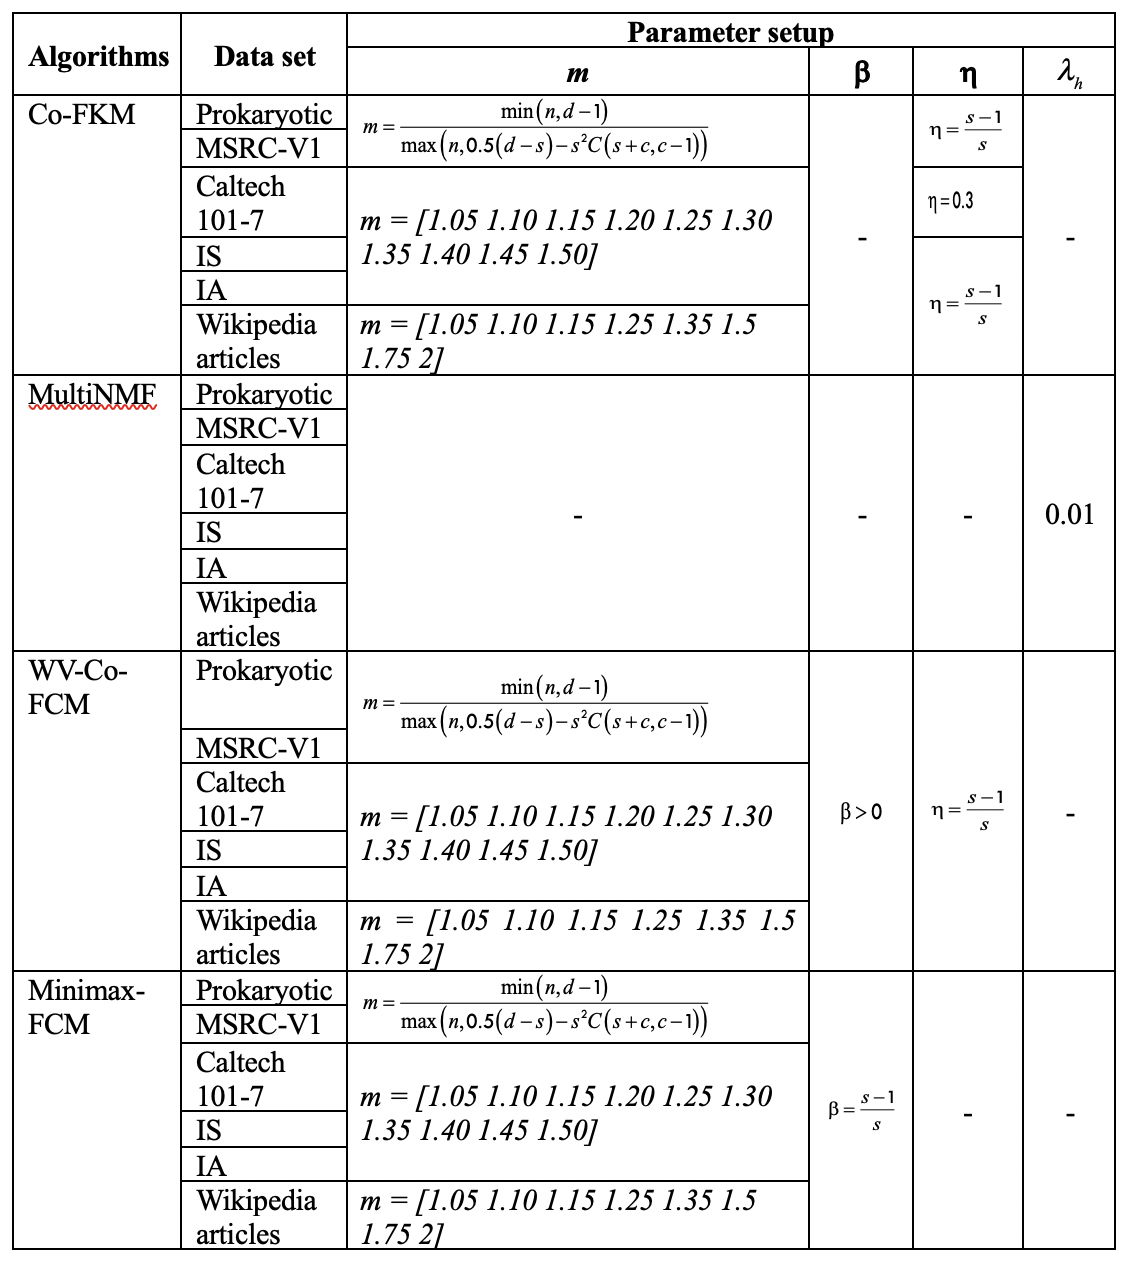
\includegraphics[width=7cm]{Table 5.2.png}
\end{figure}

\end{frame}
%---------------------------------------------------------------------------------------------------------------------------


\begin{frame}{Result: Analysis of the incorporated idea }
\vspace{-0.35cm}	
\begin{itemize}
\item Performance comparison of m ranges from 1.05 to 2 with step 0.05 for a two-view numerical data set with 4 clusters and 3 feature components on FW-MVFCM
\end{itemize}

\begin{figure}
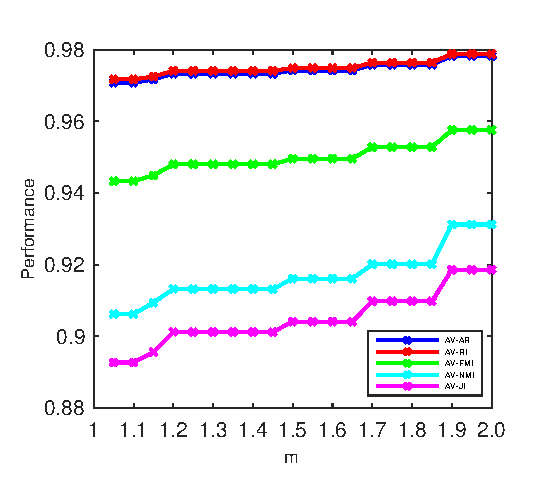
\includegraphics[width=6cm]{4c_AR.eps}
\end{figure}
\end{frame}
%---------------------------------------------------------------------------------------------------------------------------

\begin{frame}{Result: Analysis of the incorporated idea }
\vspace{-0.35cm}
\begin{itemize}
\item \scriptsize{Equal initial feature-view weights, AR, RI, FMI, NMI, and JI for different iterations of  a two-view numerical data set with 4 clusters and 3 feature components}
\end{itemize}
\begin{figure}
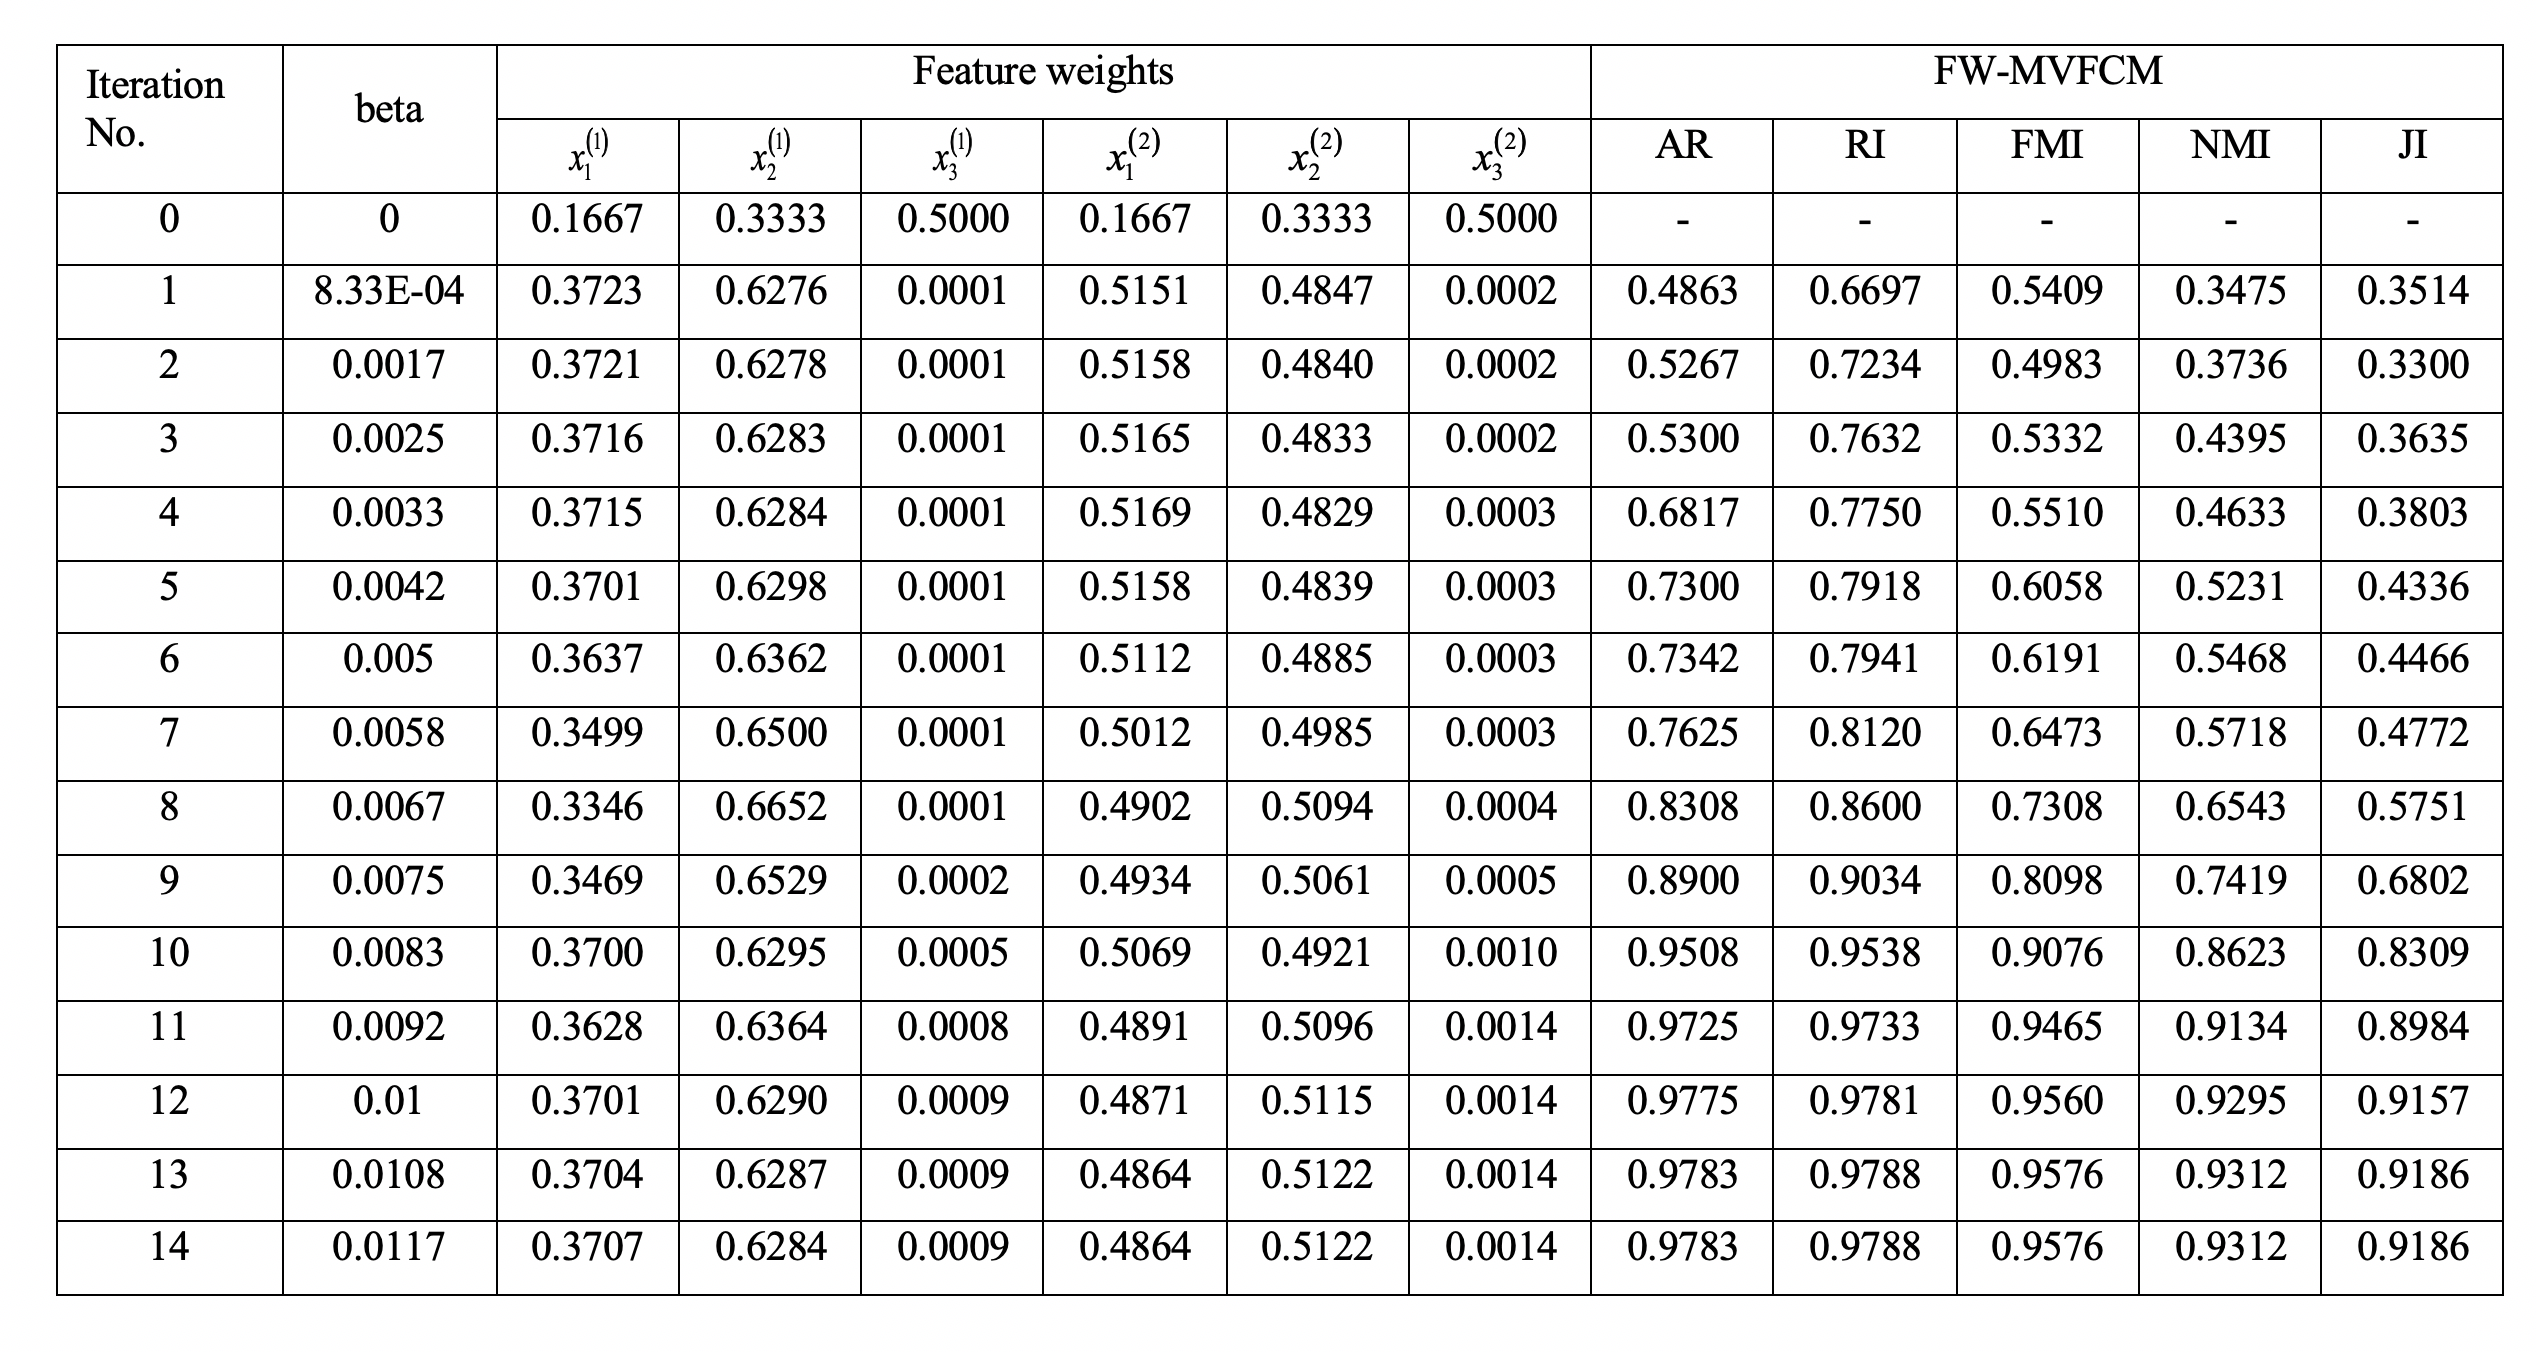
\includegraphics[width=10cm]{Table 5.3.png}
\end{figure}
\end{frame}
%---------------------------------------------------------------------------------------------------------------------------

\begin{frame}{Result: Analysis of the incorporated idea }
\begin{itemize}
\item \scriptsize{Different initial feature-view weights, AR, RI, FMI, NMI, and JI for different iterations of a two-view numerical data set with 4 clusters and 3 feature components}
\end{itemize}

\begin{figure}
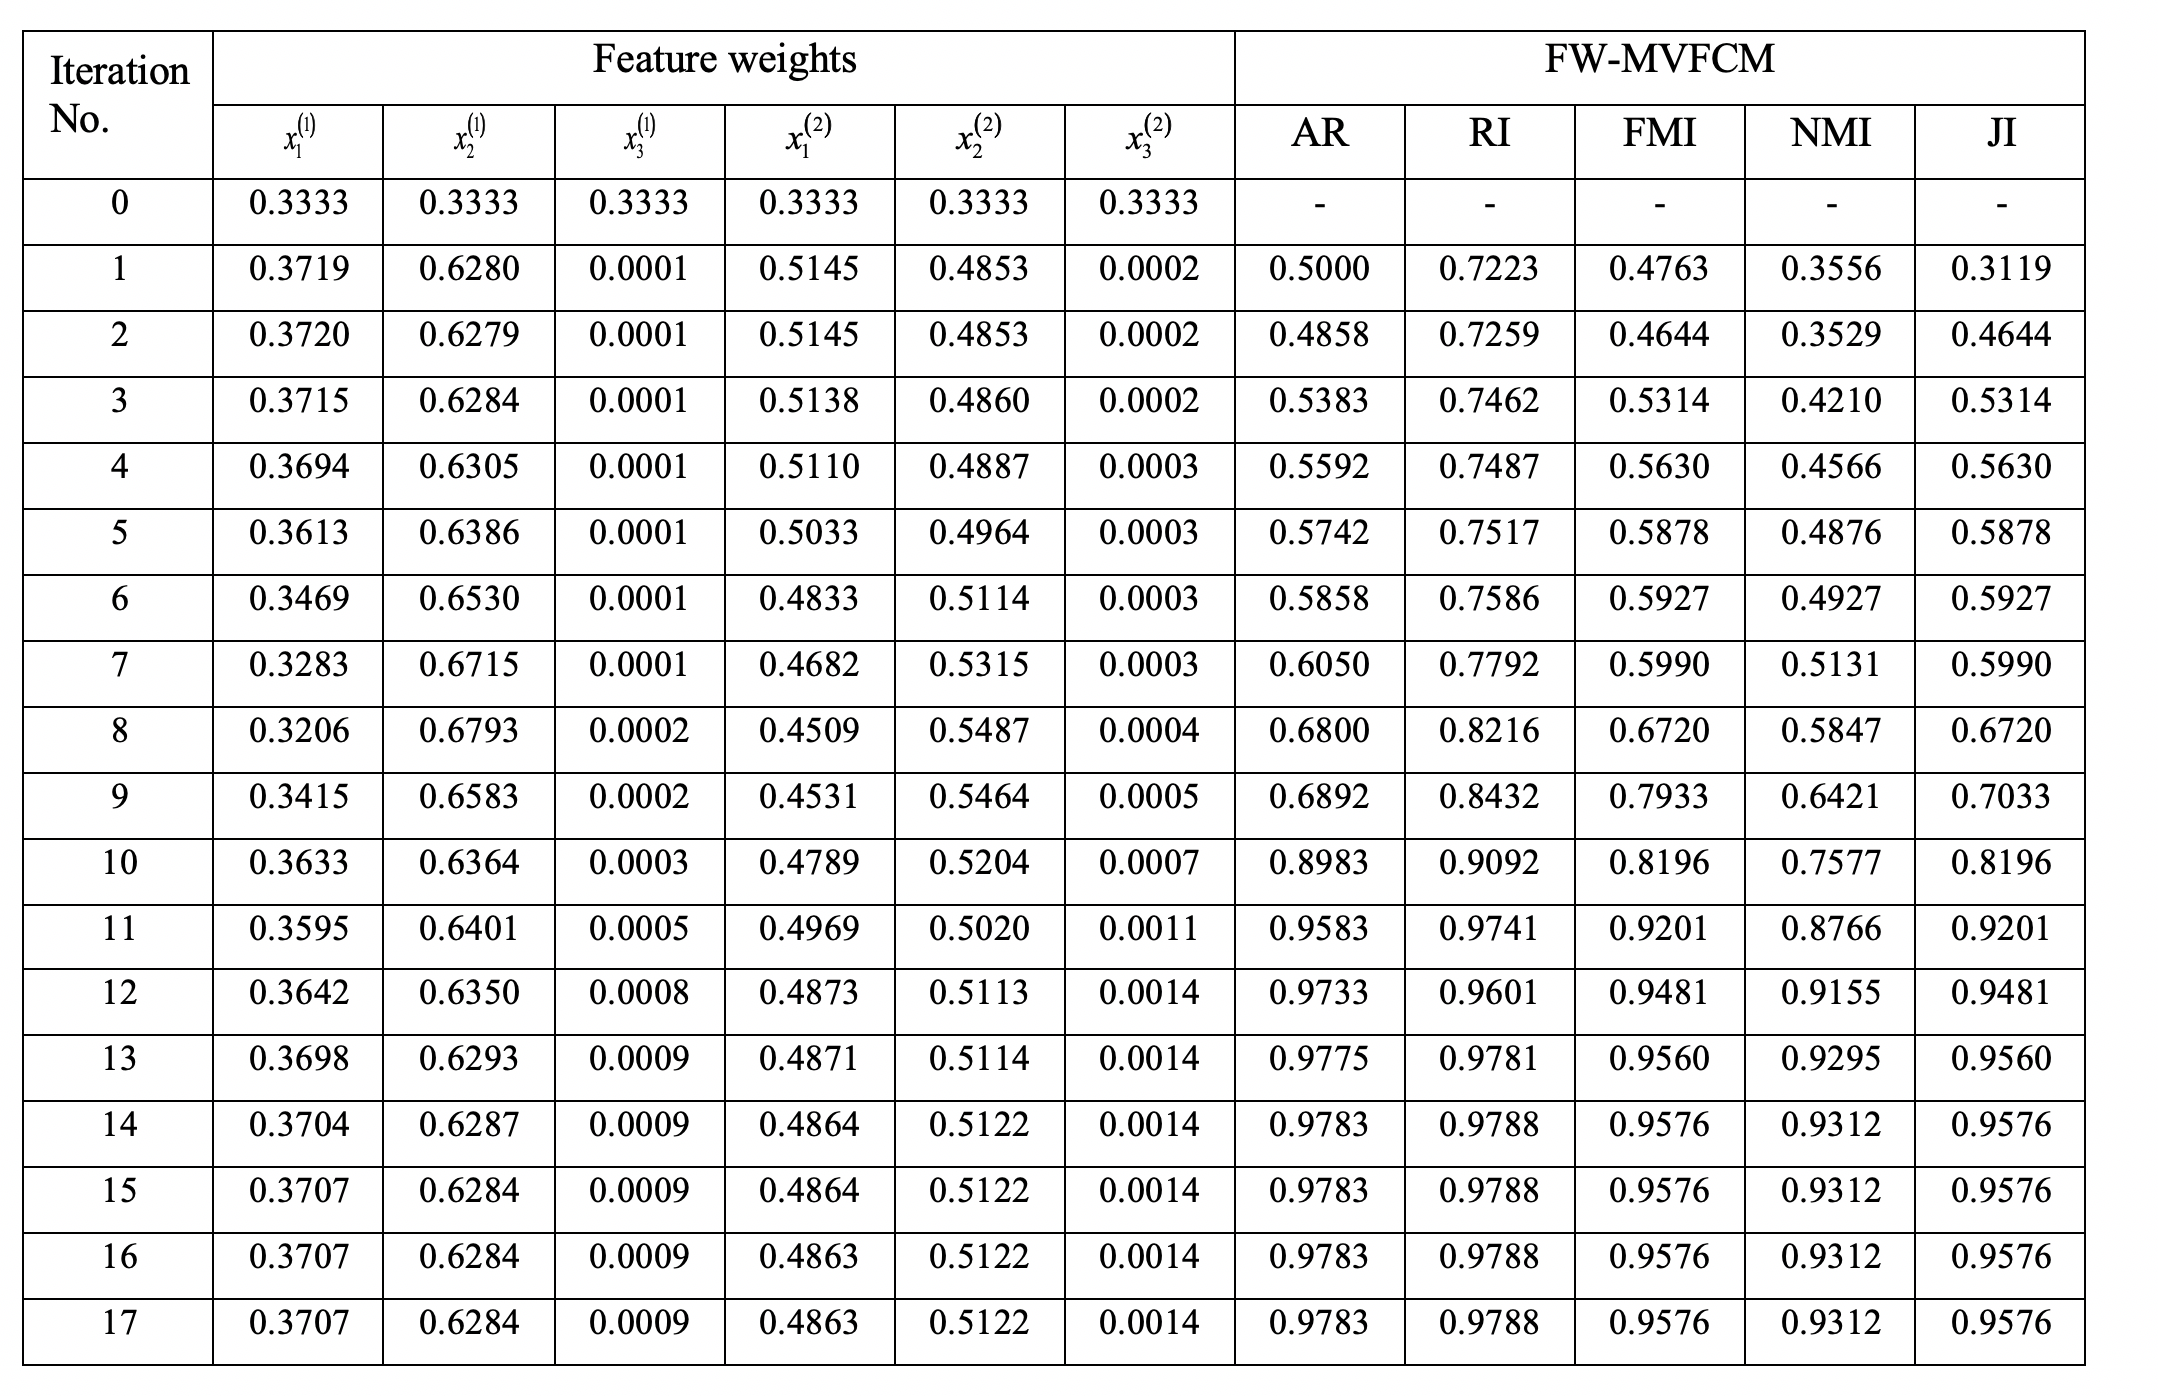
\includegraphics[width=8cm]{Table 5.4.png}
\end{figure}
\end{frame}
%---------------------------------------------------------------------------------------------------------------------------

\begin{frame}{Result:  }

\begin{itemize}
\item \scriptsize{Different initial feature-view weights, AR, RI, FMI, NMI, and JI of Co-FW-MVFCM without feature reduction (FR) for different iterations of a two-view numerical data set with 4 clusters and 3 feature components
}
\end{itemize}

\begin{figure}
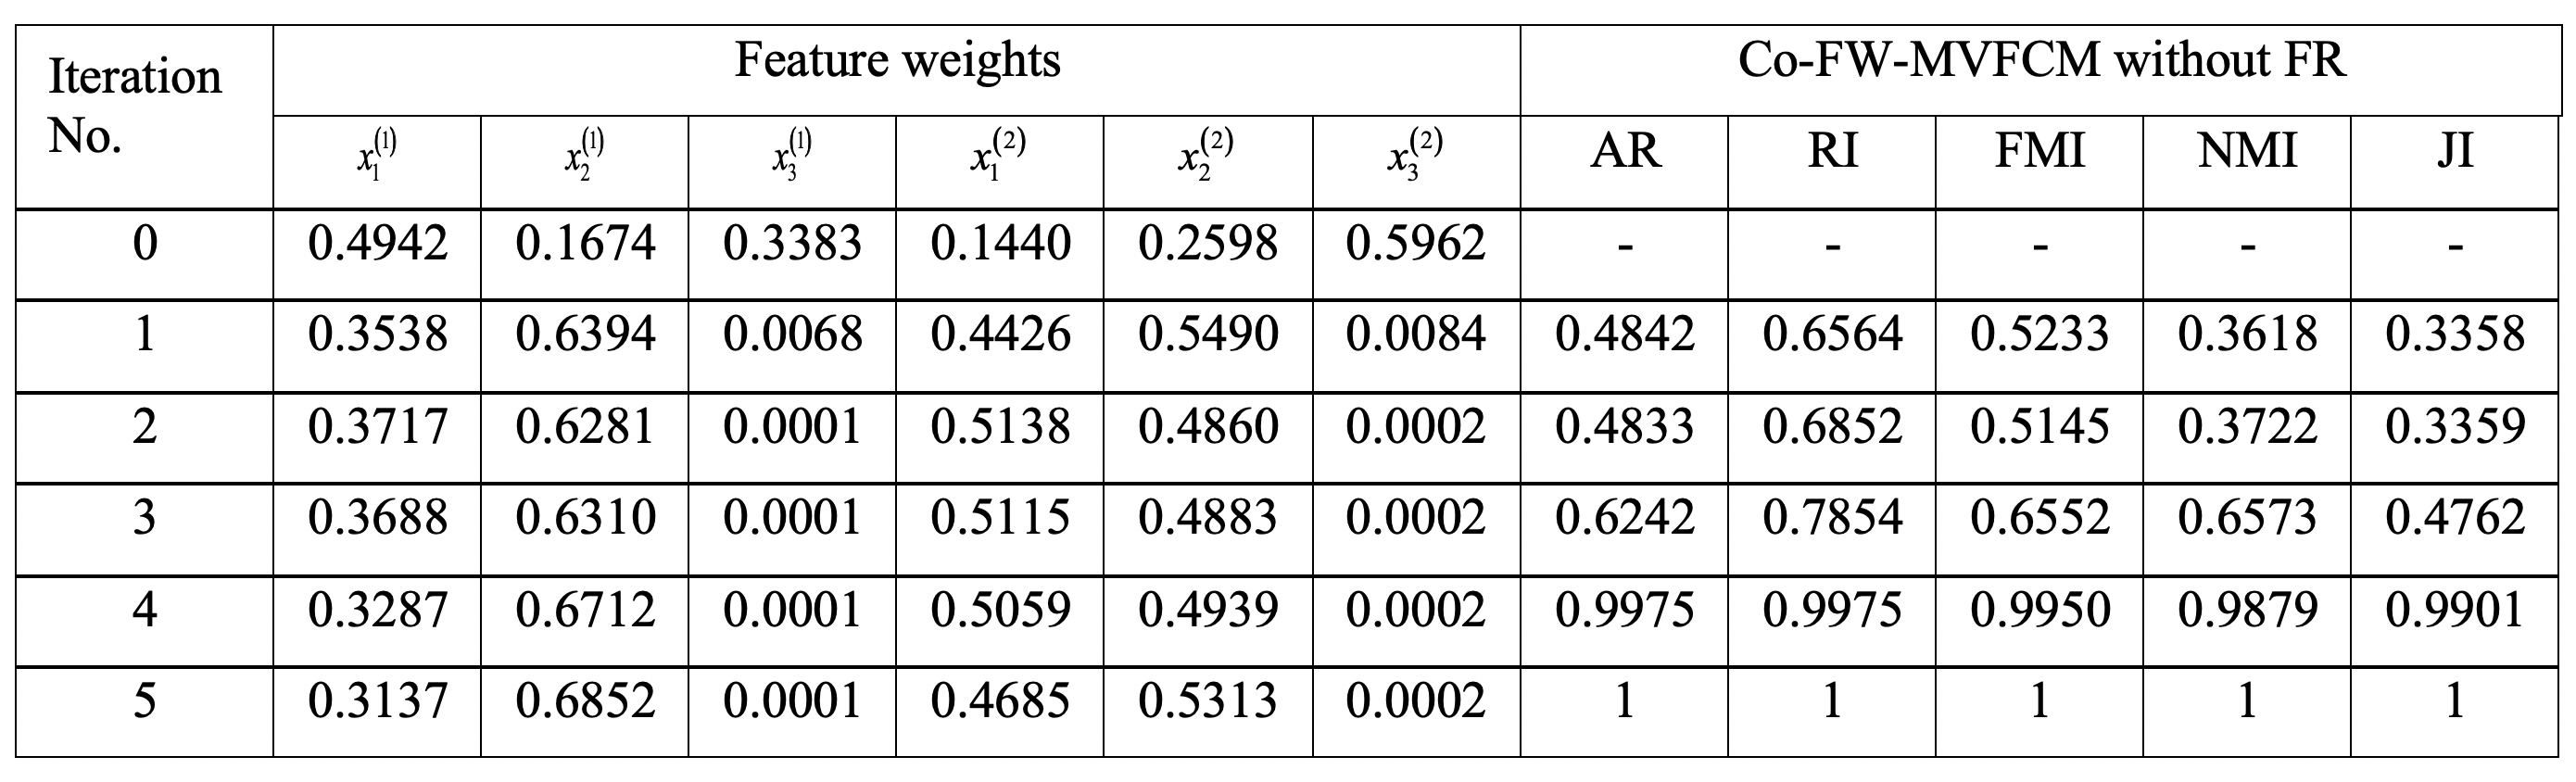
\includegraphics[width=11cm]{Table 5.5.png}
\end{figure}
\end{frame}
%---------------------------------------------------------------------------------------------------------------------------

\begin{frame}{Result:  }

\begin{itemize}
\item \scriptsize{Different initial feature-view weights, AR, RI, FMI, NMI, and JI of Co-FW-MVFCM with feature reduction (FR) for different iterations of a two-view numerical data set with 4 clusters and 3 feature components}
\end{itemize}

\begin{figure}
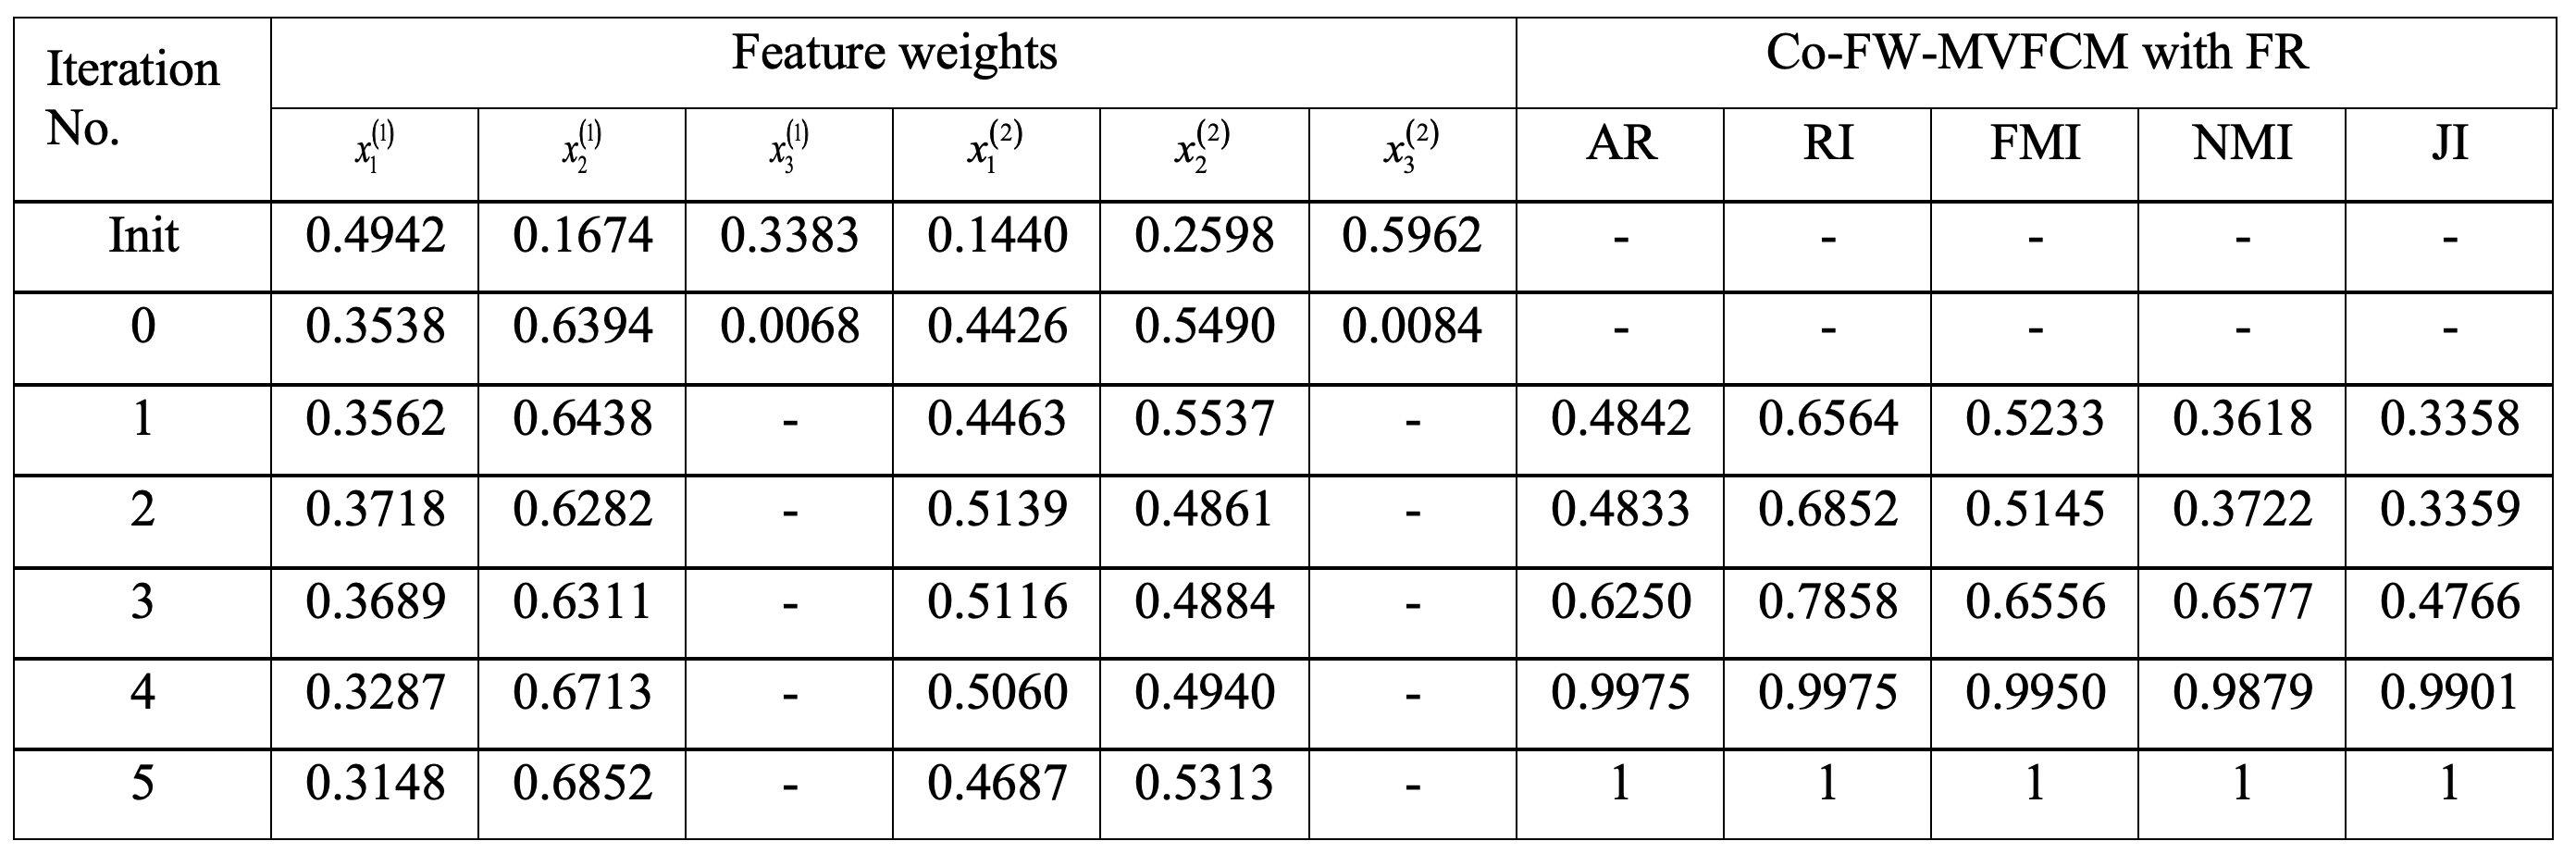
\includegraphics[width=11cm]{Table 5.6.png}
\end{figure}
\end{frame}
%---------------------------------------------------------------------------------------------------------------------------

\begin{frame}{Result:  }

\begin{itemize}
\item \scriptsize{Final feature-view weights of FW-MVFCM and Co-FW-MVFCM with feature reduction (FR) of a two-view numerical data set with 4 clusters and 3 feature Components over 5 simulations}
\end{itemize}

\begin{figure}
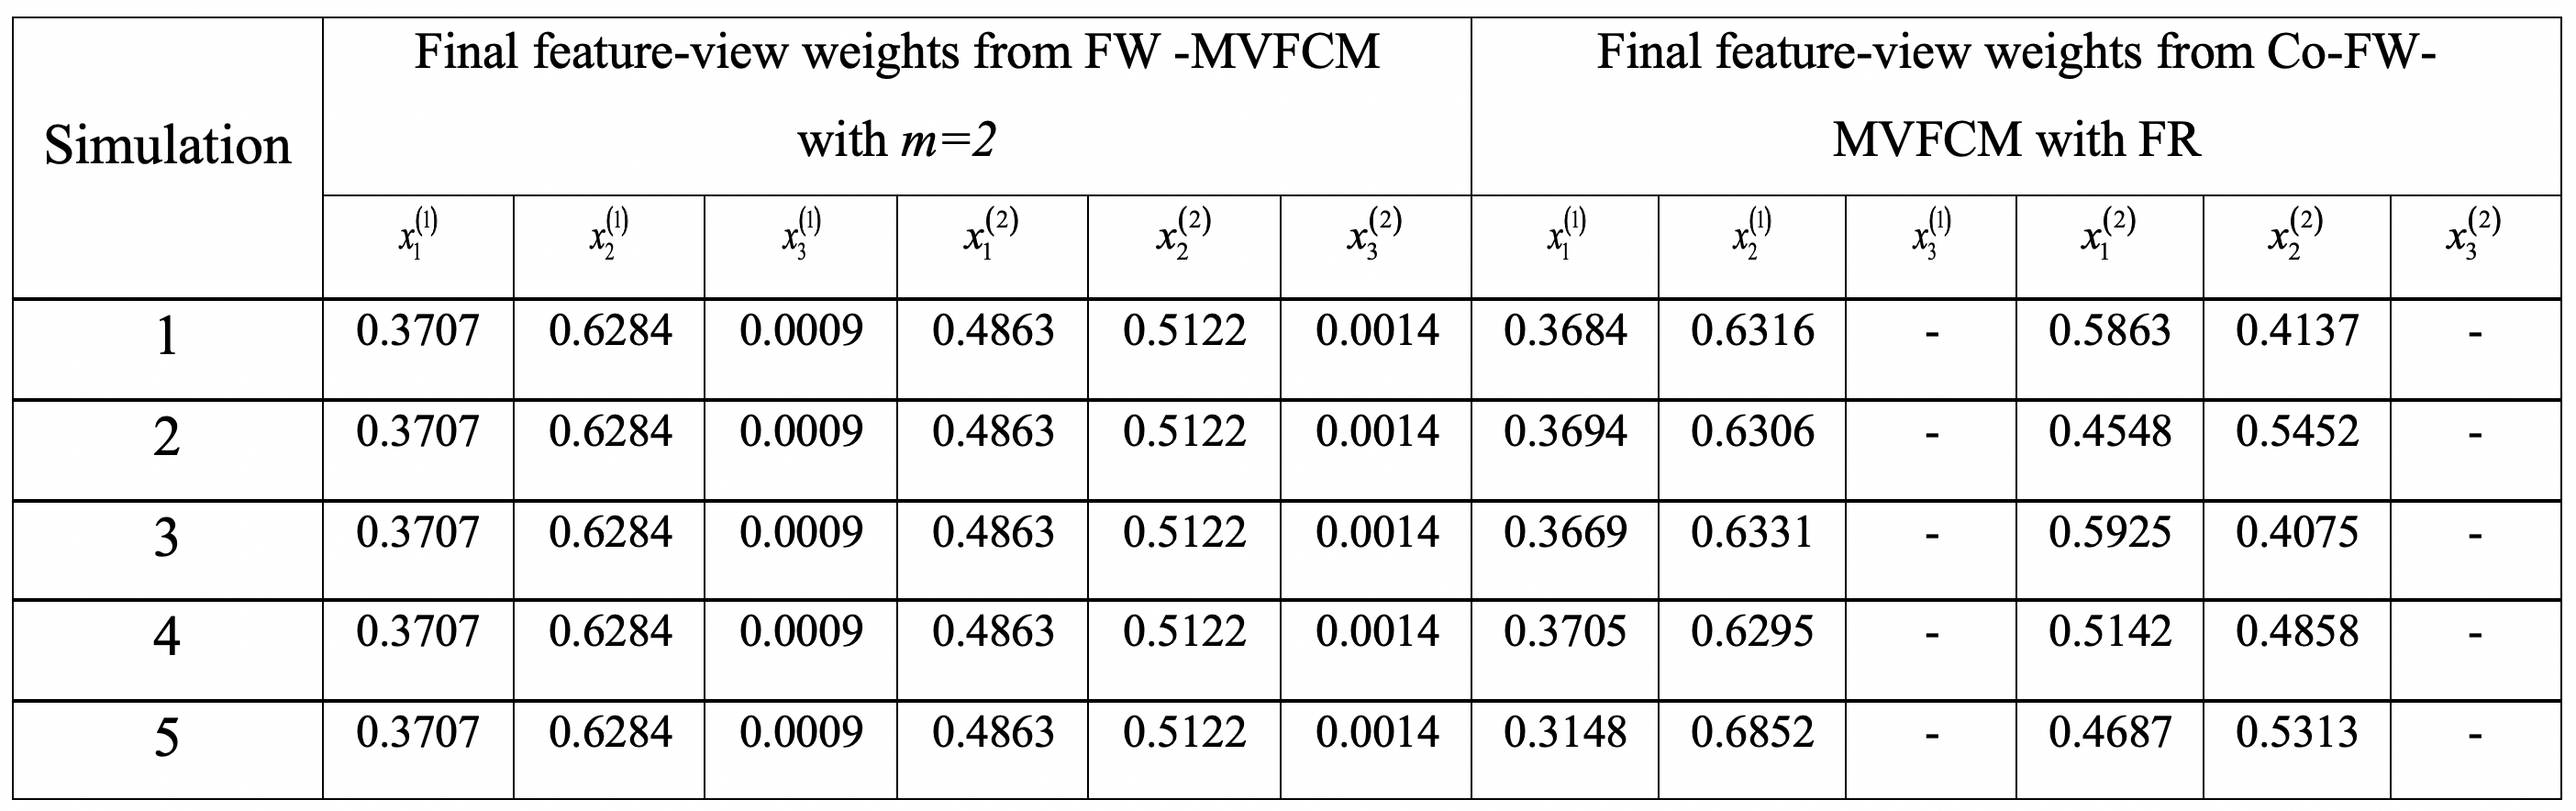
\includegraphics[width=11cm]{Table 5.7.png}
\end{figure}
\end{frame}
%---------------------------------------------------------------------------------------------------------------------------

\begin{frame}{Result:  }

\begin{itemize}
\item \scriptsize{Comparison of AR, RI, FMI, NMI, and JI between FW-MVFCM and Co-FW-MVFCM based on the simulations of Table 5.7}
\end{itemize}

\begin{figure}
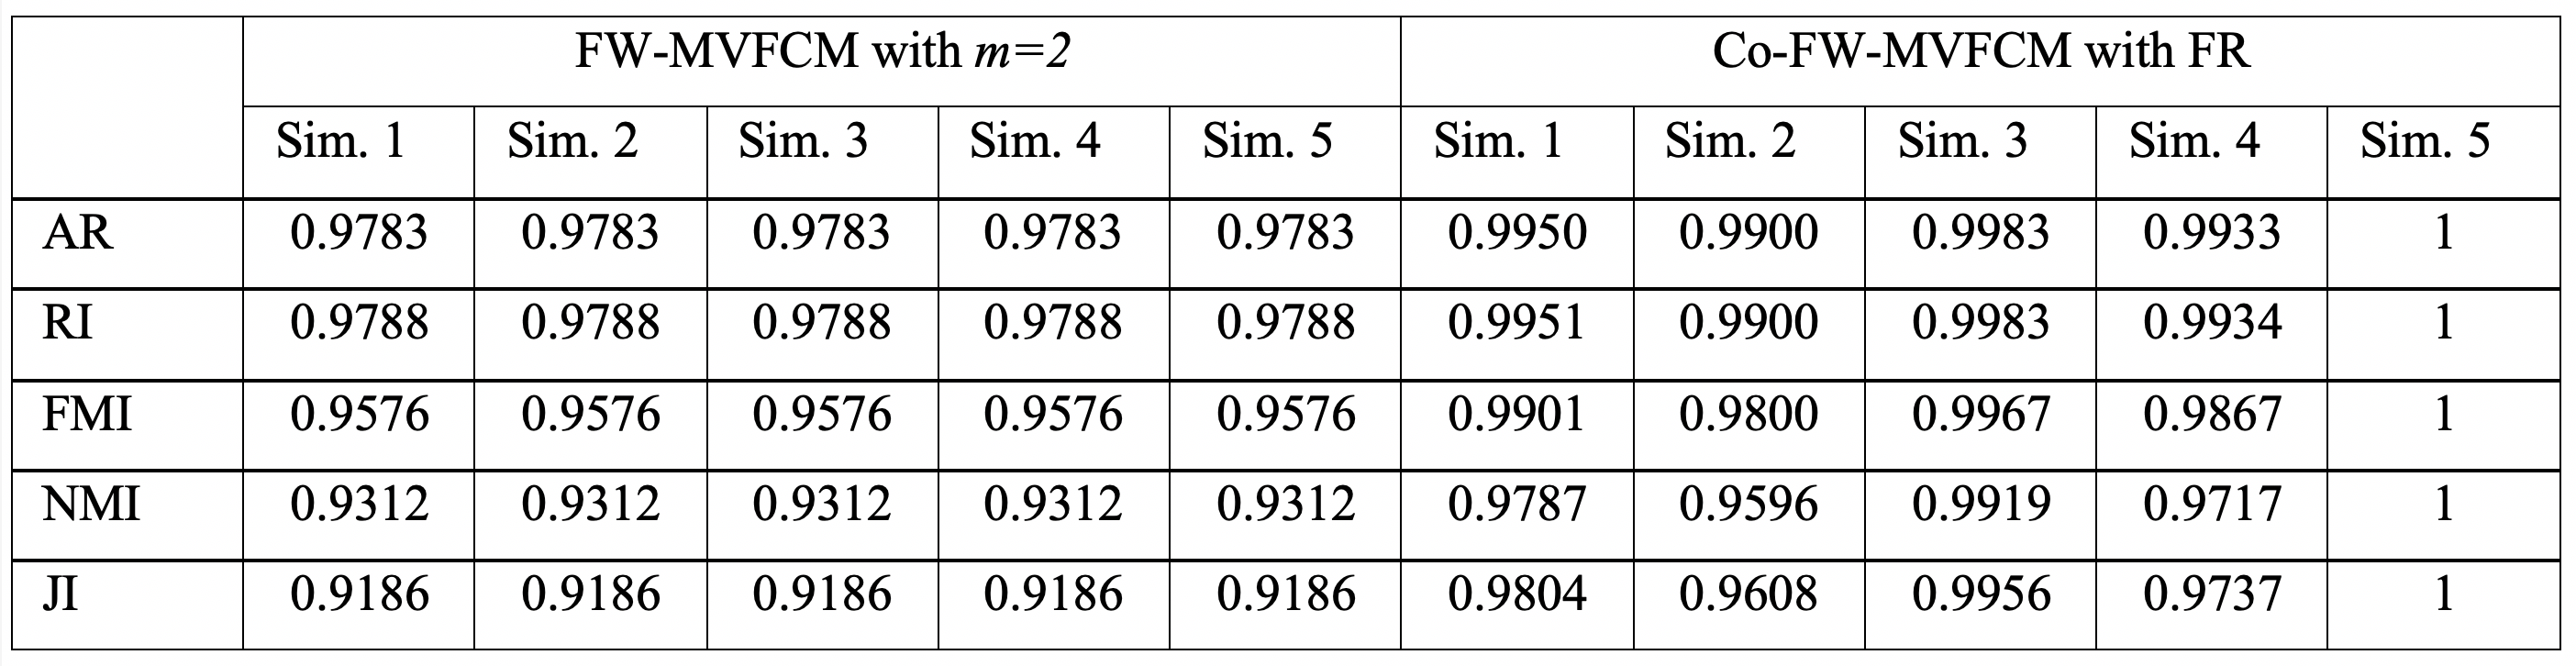
\includegraphics[width=10cm]{Table 5.8.png}
\end{figure}
\end{frame}
%---------------------------------------------------------------------------------------------------------------------------

\begin{frame}{Result:  }

\begin{itemize}
\item \footnotesize{Performance comparison of $m$ are [1.05 1.10 1.25 1.35 1.50 1.75 2] for a two-view numerical data set with 4 clusters and 3 feature components on (a) Co-FKM, (b) MinMax FCM, (c) WV-Co-FCM for the first case of $\delta_{ik}^{h}$  with $\delta_{ik}^{h} = \eta \frac{1}{s-1}\sum_{h'=1, h'\neq h}^{s}\sum_{j=1}^{d_{h}}\left(x_{ij}^{h'}-a_{kj}^{h'}\right)^2$, 
and (d) WV-Co-FCM for the second case of  $\delta_{ik}^{h}$ with $\delta_{ik}^{h} = \frac{\eta}{s}\sum_{h=1}^{s}\sum_{j=1}^{d_{h}}\left(x_{ij}^{h}-a_{kj}^{h}\right)^2$}
\end{itemize}

\end{frame}
%---------------------------------------------------------------------------------------------------------------------------


\begin{frame}{Result:  }

\begin{figure}
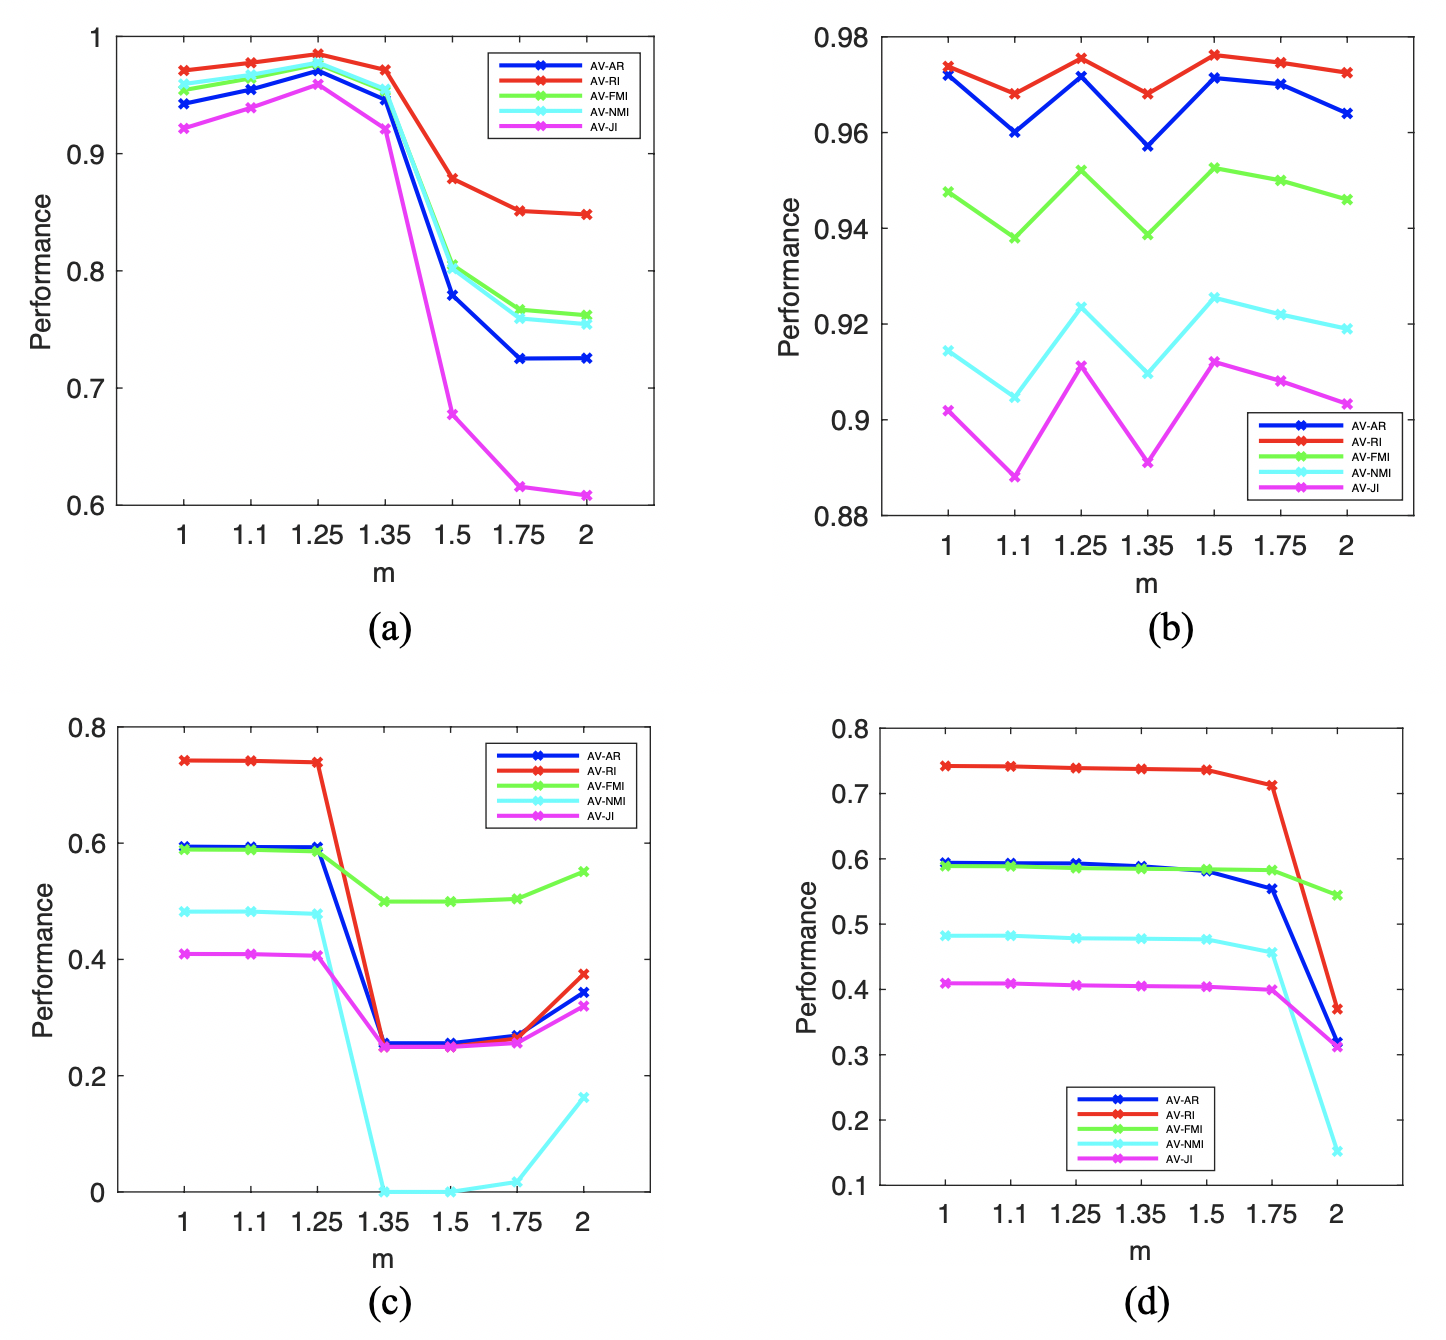
\includegraphics[width=7cm]{Fig. 5.2 .png}
\end{figure}

\end{frame}

%---------------------------------------------------------------------------------------------------------------------------

\begin{frame}{Result:  }

\begin{itemize}
\item \scriptsize{Performance comparison of m ranges from 1.05 to 1.5 and $\eta=s-1/s$ for (a) Co-FKM; (b) WV-Co-FCM; and (c) Minimax-FCM on Caltech 101 data set.}
\end{itemize}

\begin{figure}
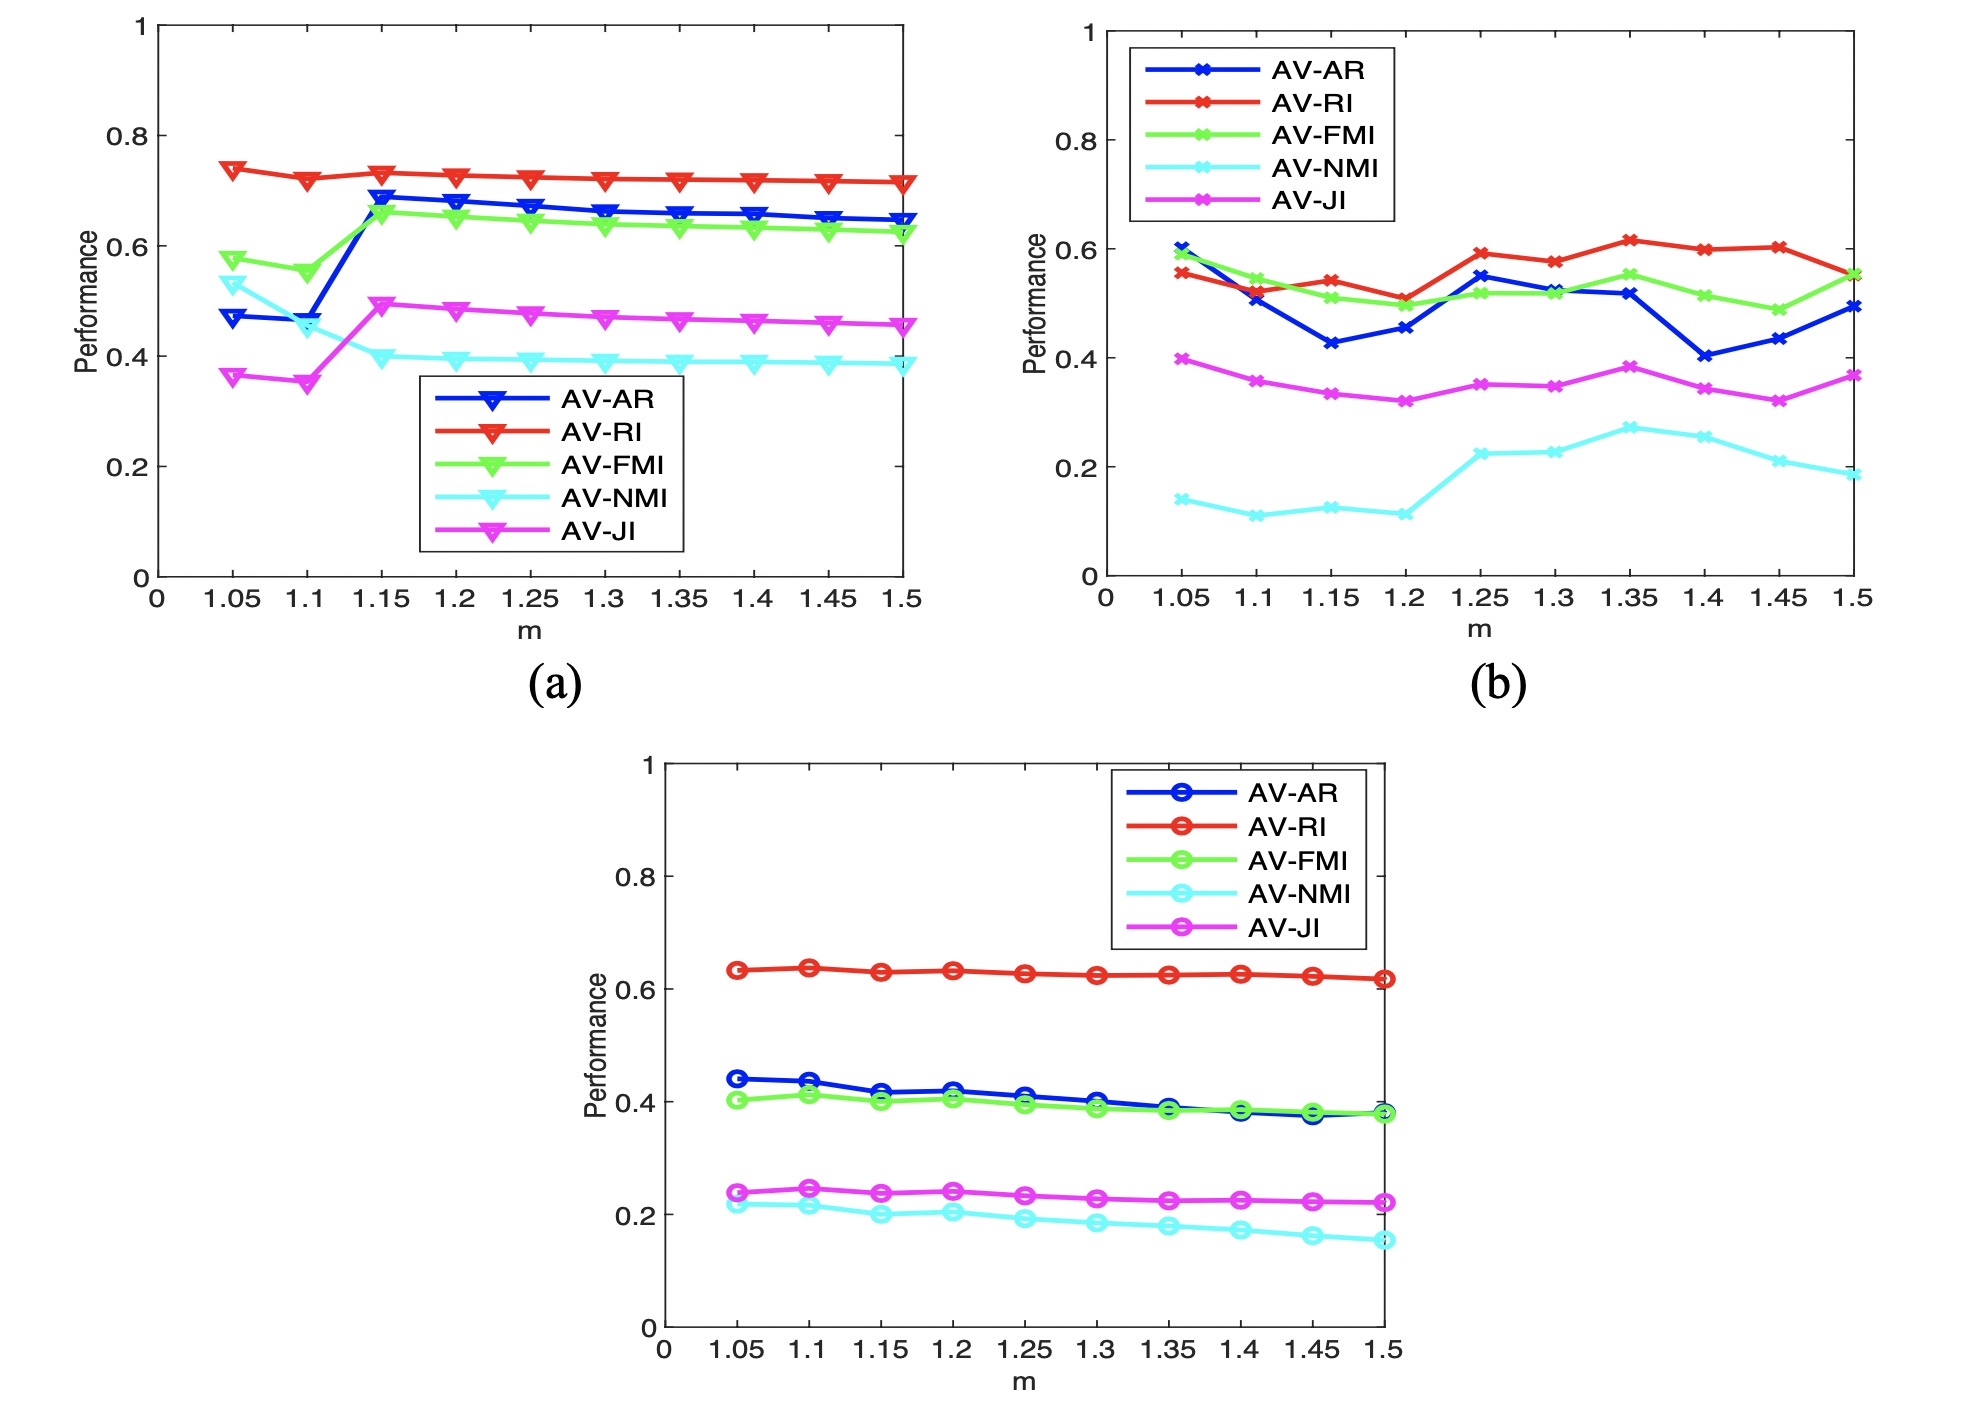
\includegraphics[width=8cm]{Fig. 5.3 .png}
\end{figure}
\end{frame}
%---------------------------------------------------------------------------------------------------------------------------

\begin{frame}{Result:  }

\begin{itemize}
\item \scriptsize{Performance comparison of m ranges from 1.05 to 2 and $\eta=s-1/s$  for (a) Co-FKM; (b) WV-Co-FCM; and (c) Minimax-FCM on Wikipedia Articles data set.}
\end{itemize}


\begin{figure}
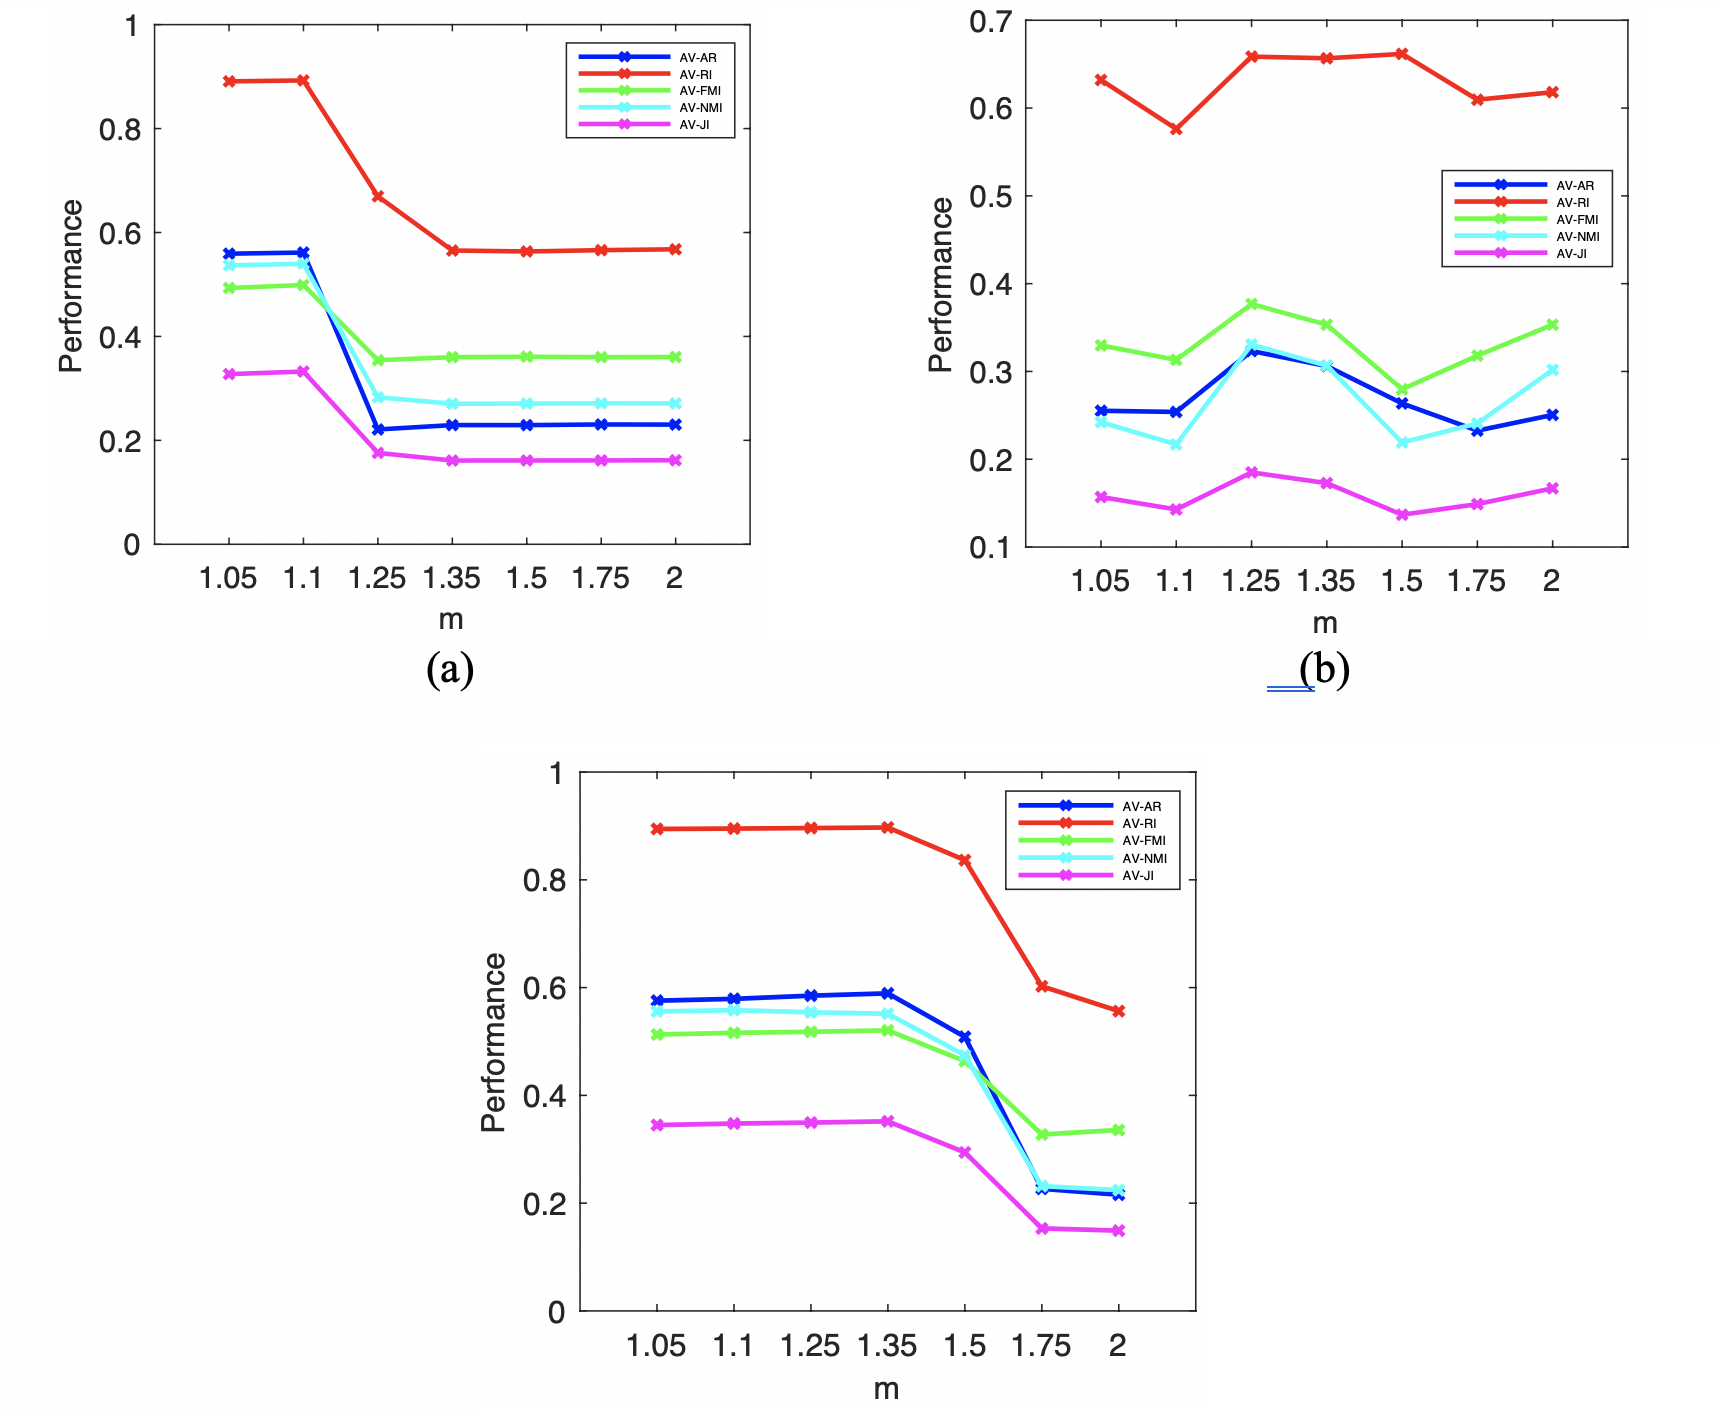
\includegraphics[width=7cm]{Fig. 5.4 .png}
\end{figure}
\end{frame}
%---------------------------------------------------------------------------------------------------------------------------

\begin{frame}{Result:  }

\begin{itemize}
\item \scriptsize{Classification results of CoFKM, MultiNMF, WV-Co-FCM, Minimax FCM, and the proposed Co-FW-MVFCM algorithms in Prokaryotic Phyla and MSRC-V124 multi-view data sets}
\end{itemize}


\begin{figure}
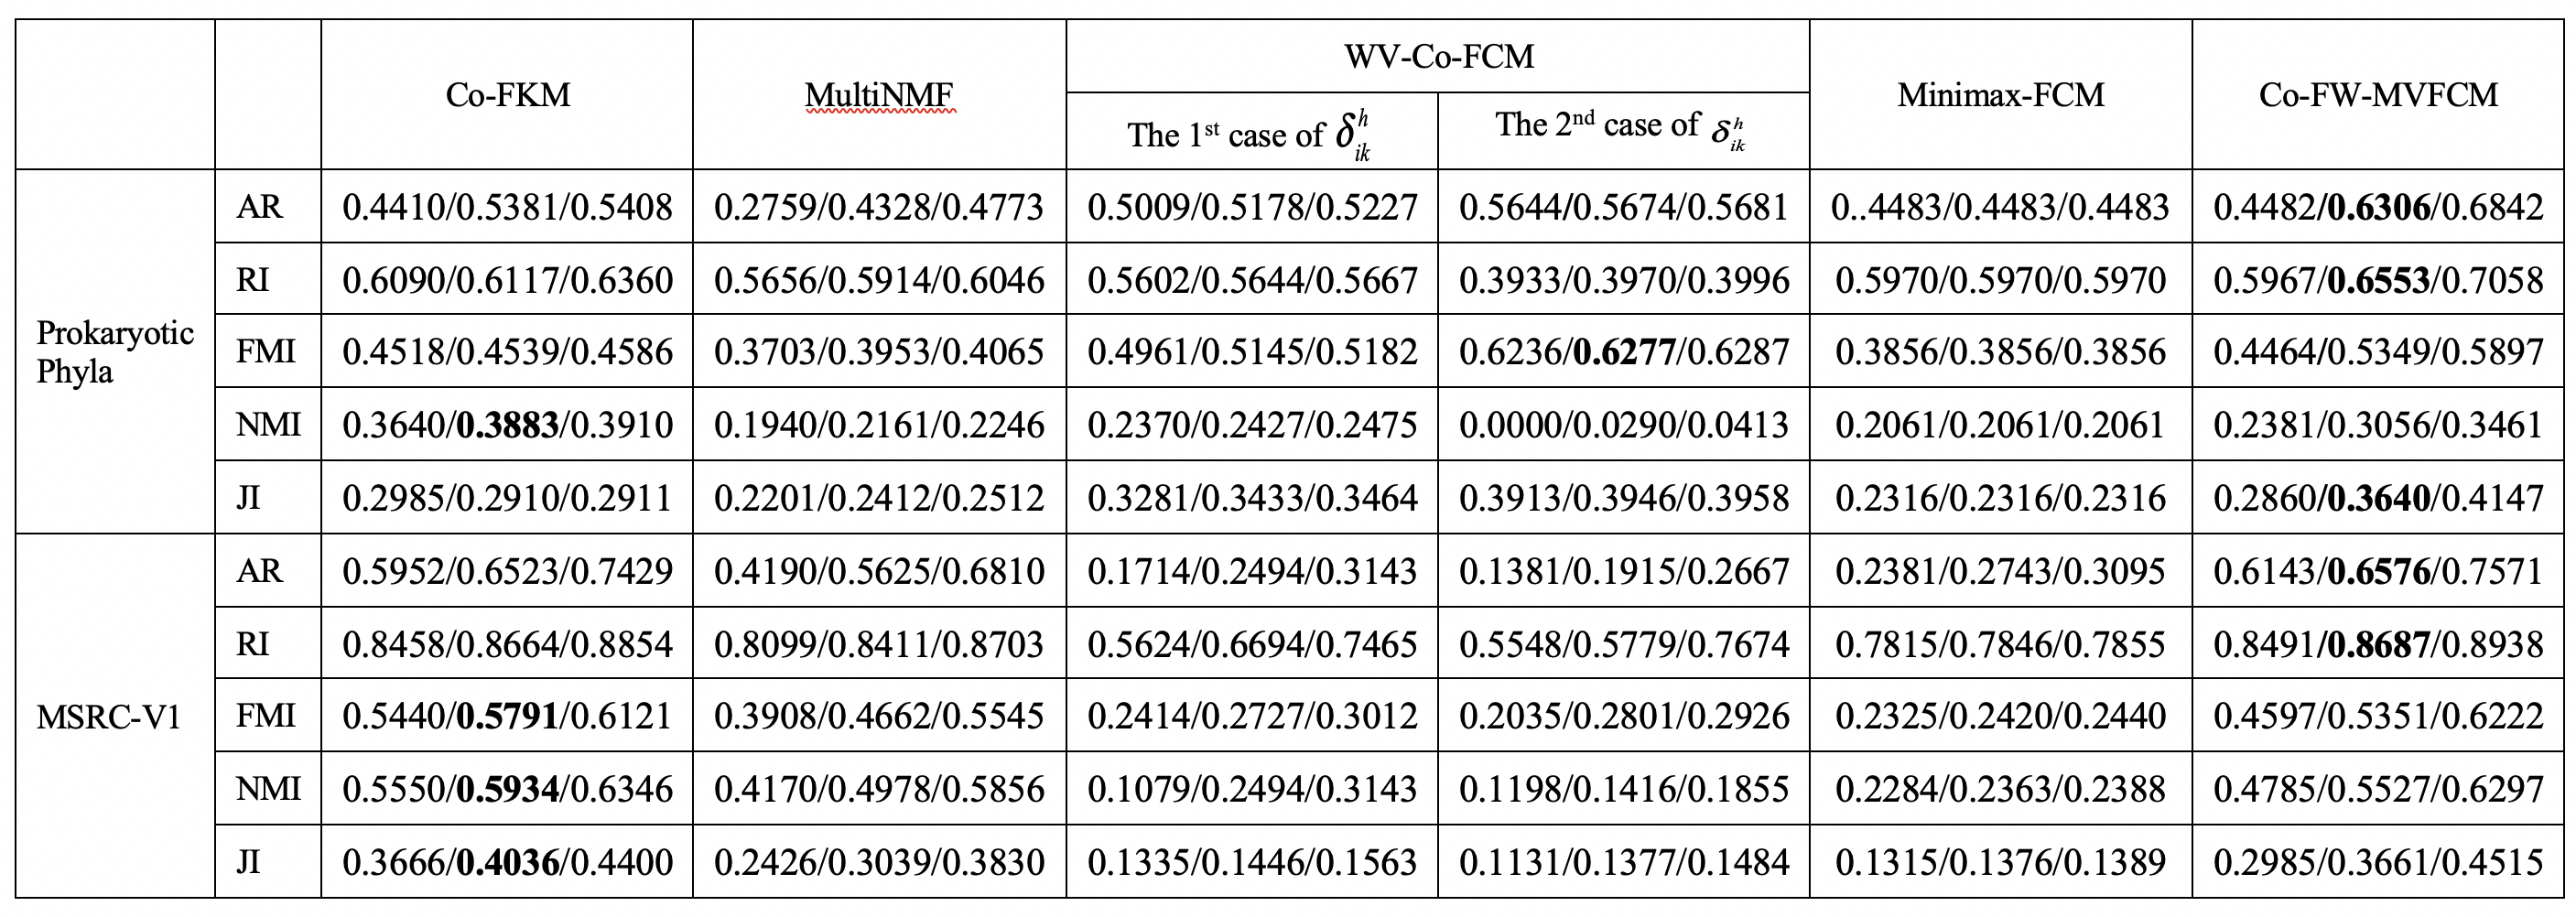
\includegraphics[width=10cm]{Table 5.9.png}
\end{figure}
\end{frame}
%---------------------------------------------------------------------------------------------------------------------------

\begin{frame}{Result:  }
\vspace{-0.5cm}
\begin{itemize}
\item \scriptsize{Classification results of CoFKM, MultiNMF, WV-Co-FCM, Minimax FCM, and the proposed Co-FW-MVFCM algorithms in Caltech 101-7, Image segmentation (IS), and Internet advertisement (IA) multi-view data sets}
\end{itemize}


\begin{figure}
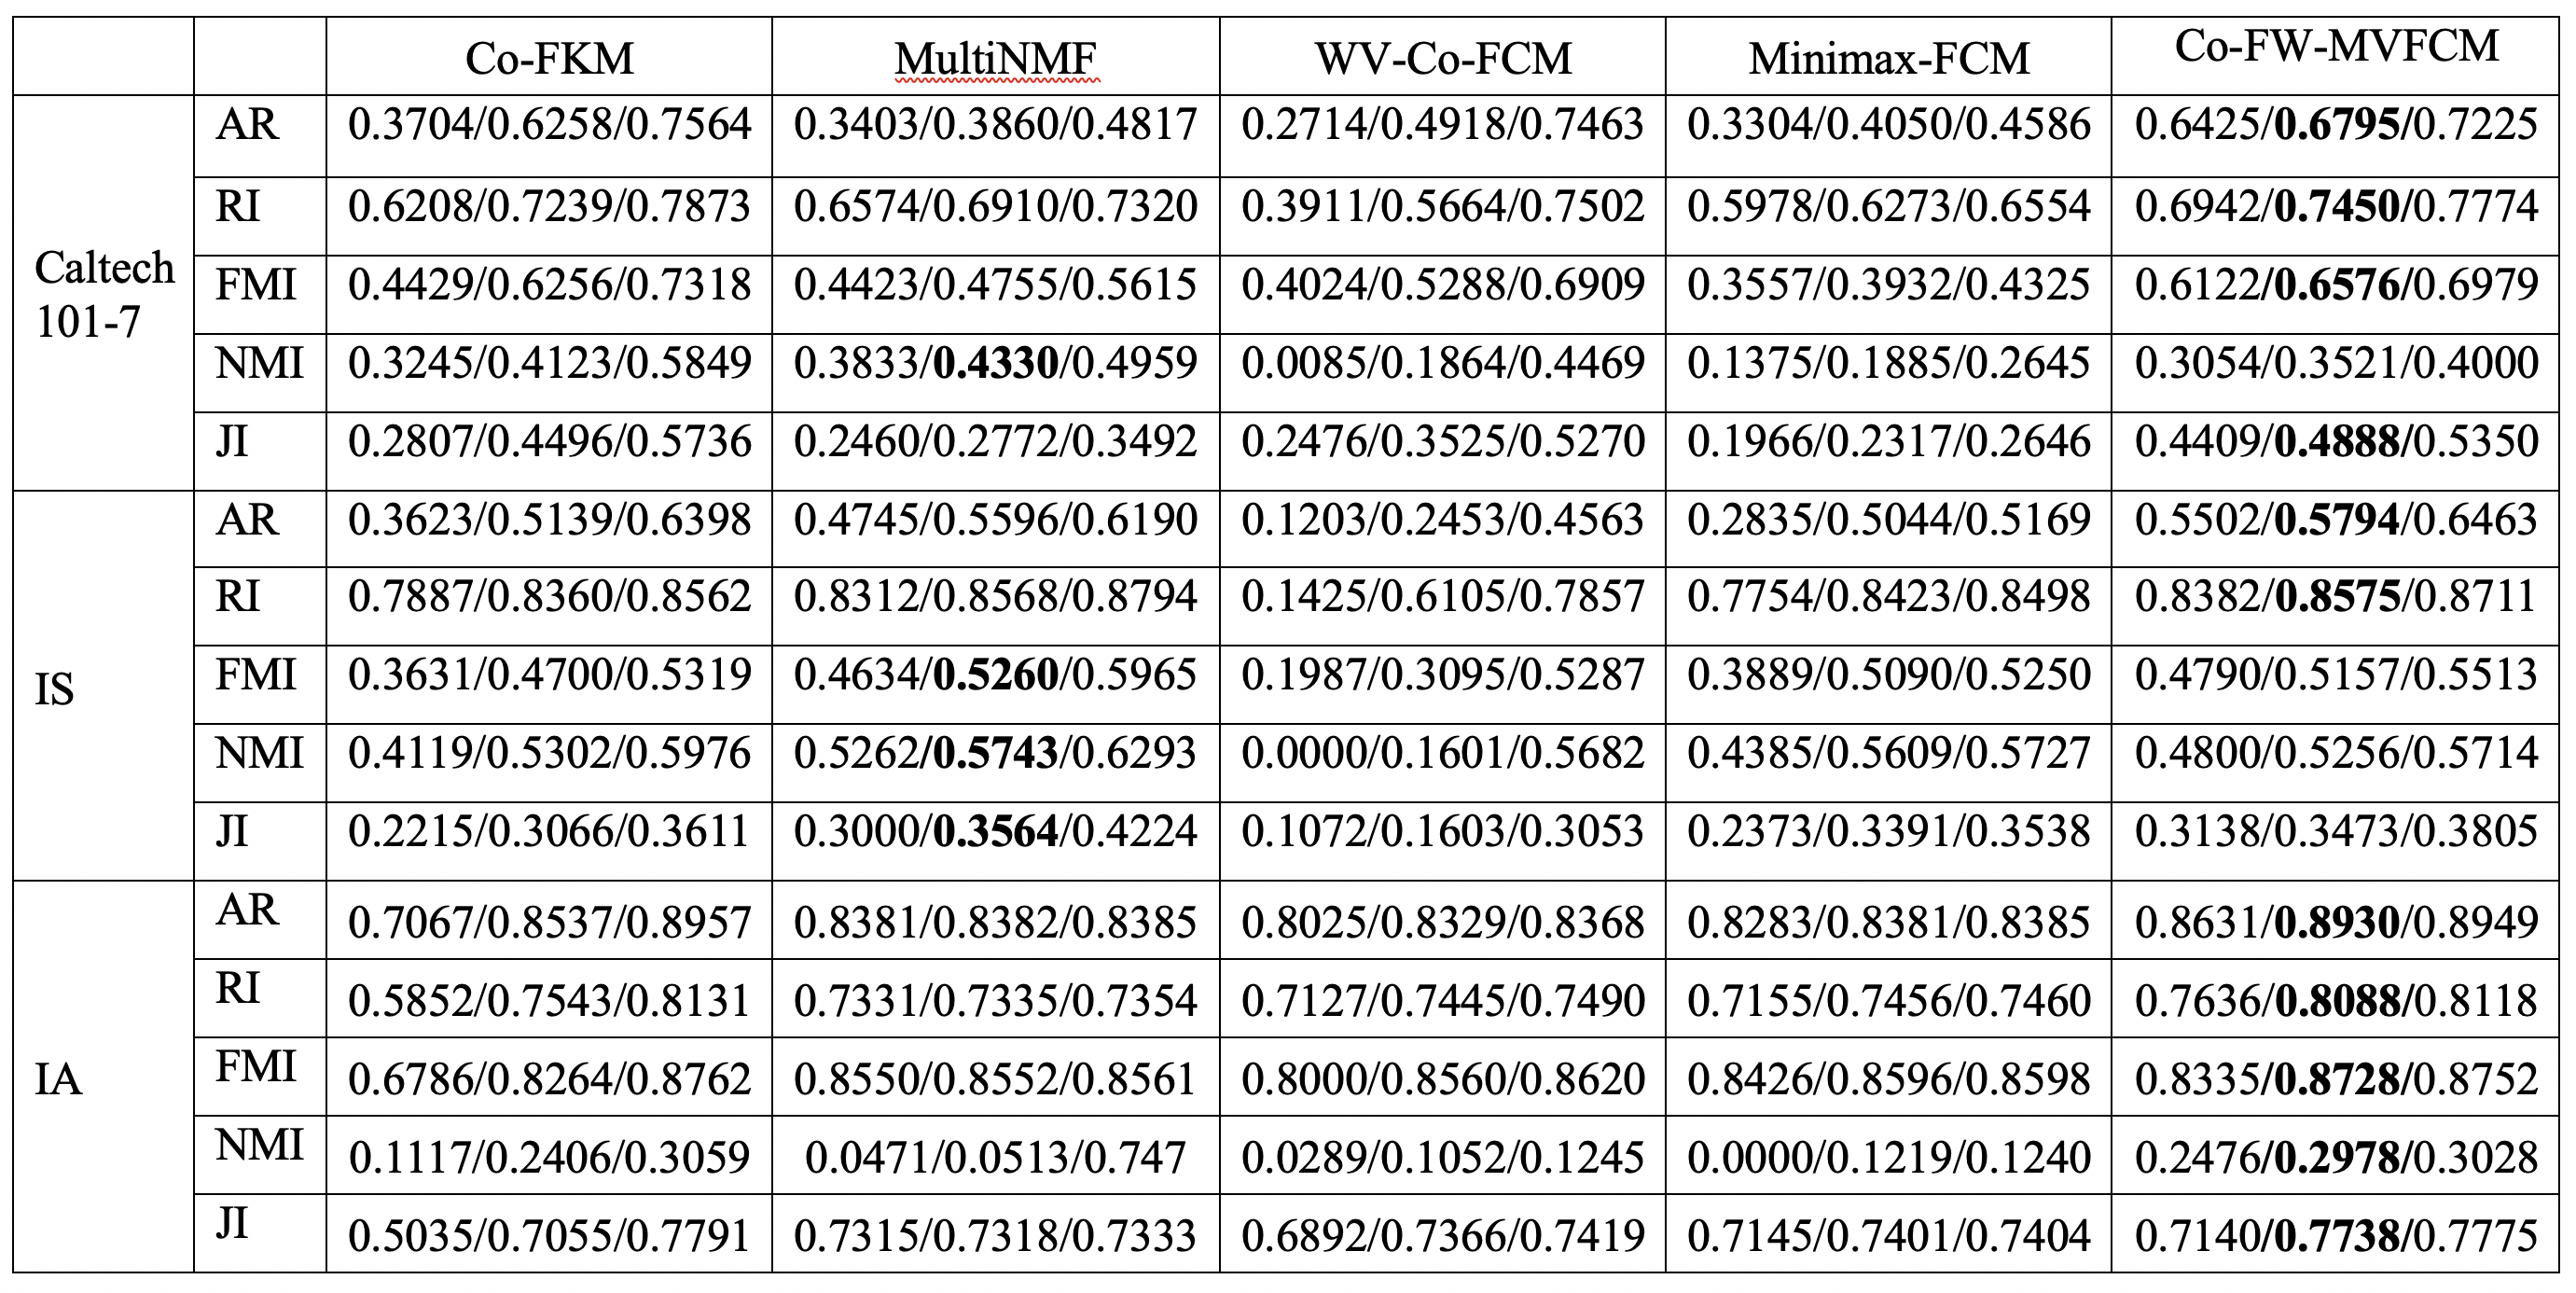
\includegraphics[width=10cm]{Table 5.10.png}
\end{figure}
\end{frame}
%---------------------------------------------------------------------------------------------------------------------------

\begin{frame}{Result:  }
\vspace{-0.5cm}
\begin{itemize}
\item \scriptsize{Classification results of MultiNMF and the proposed Co-FW-MVFCM algorithms in Wikipedia Articles multi-view data set}
\end{itemize}
\begin{figure}
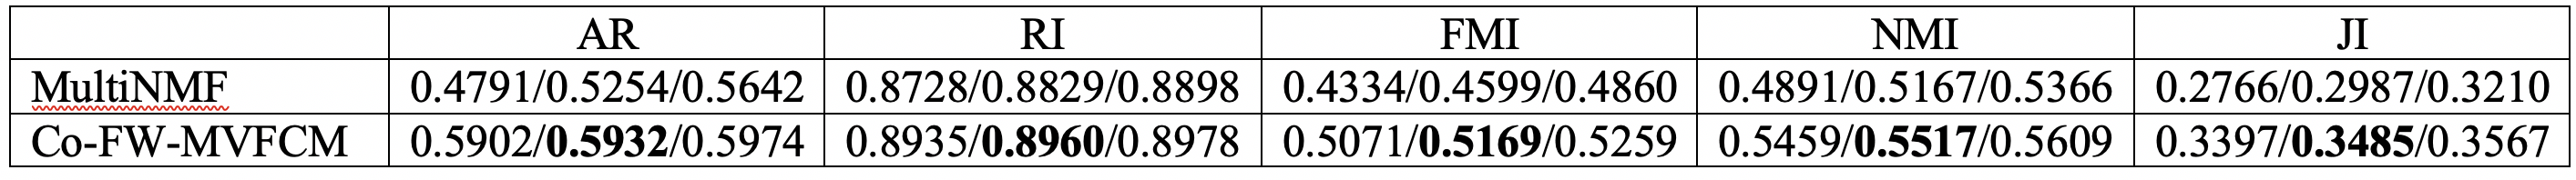
\includegraphics[width=10cm]{Table 5.11.png}
\end{figure}
\begin{itemize}
\item \scriptsize{Results of final features of the proposed Co-FW-MVFCM}
\end{itemize}
\begin{figure}
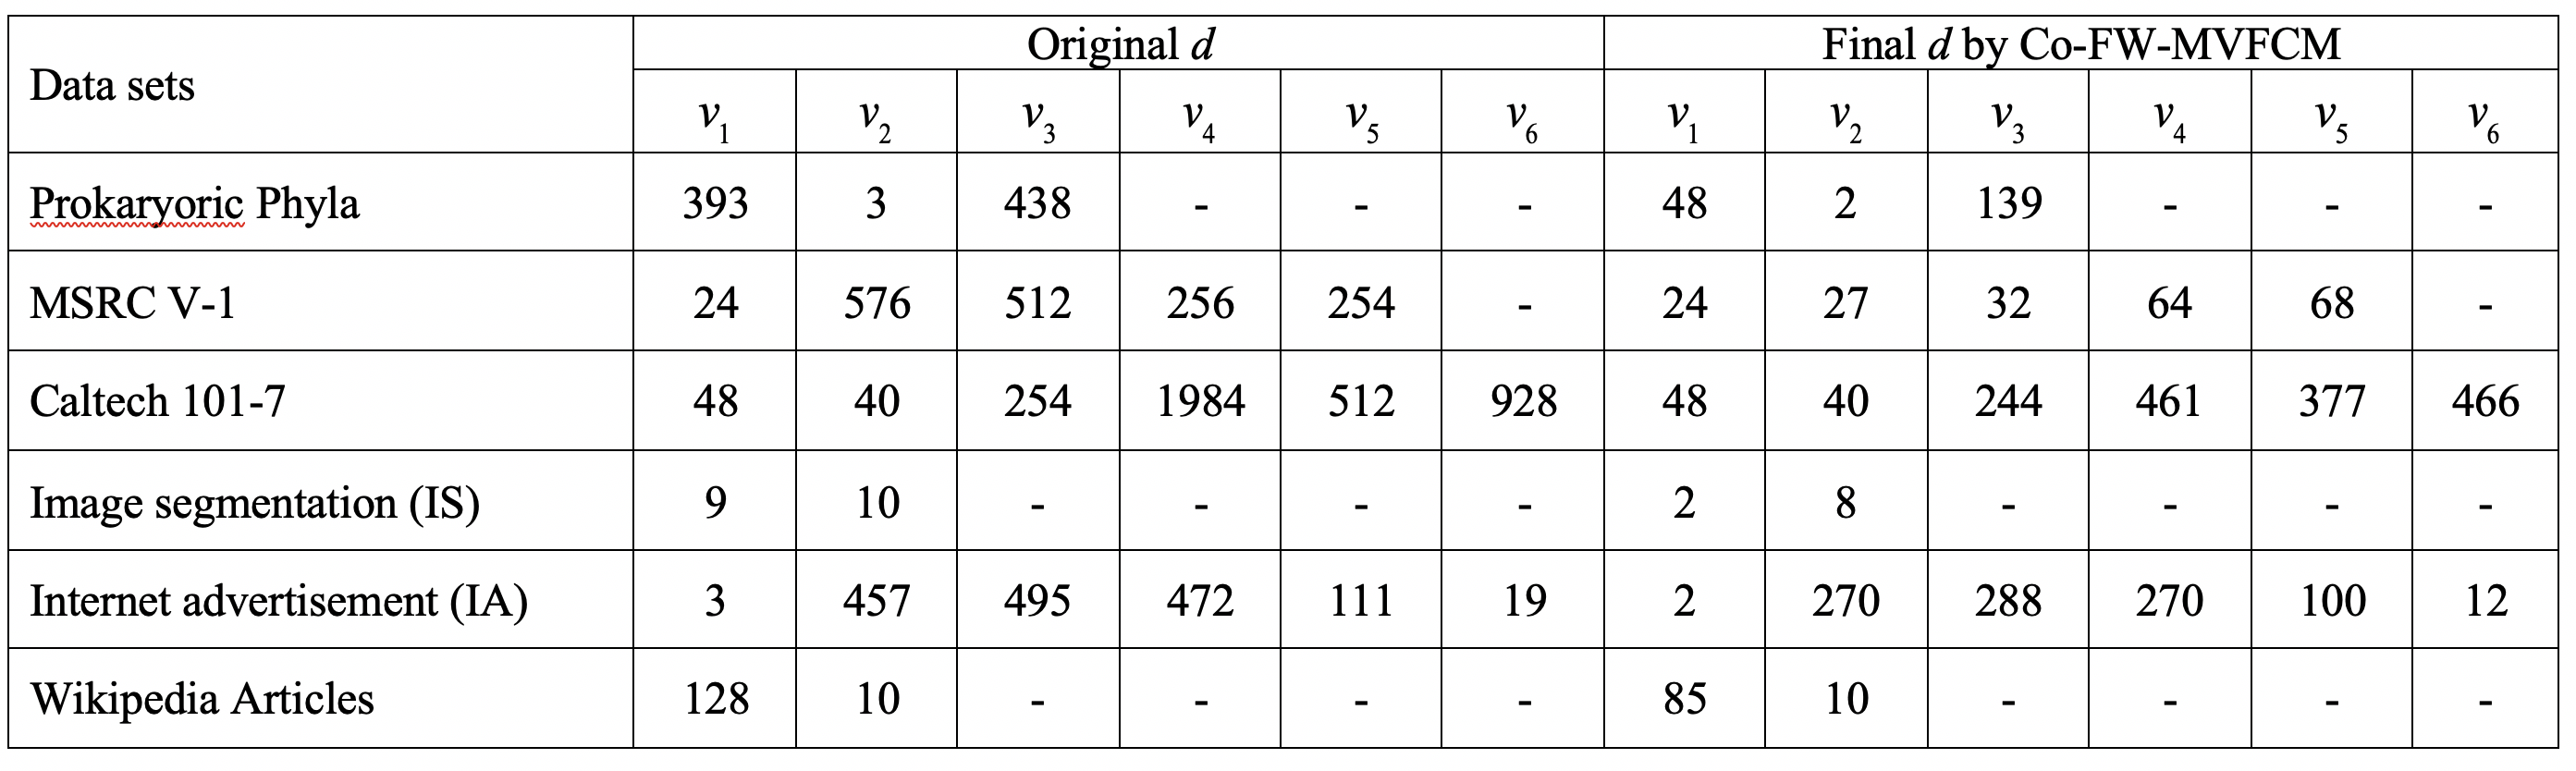
\includegraphics[width=10cm]{Table 5.12.png}
\end{figure}
\end{frame}
%---------------------------------------------------------------------------------------------------------------------------

% =================================================================

\begin{frame}{}
    \centering
    \Huge{\textbf{Conclusions}}
\end{frame}
% =================================================================

%%%%%%%%%%%%%%%%%%%%%%%%%%%%%%%%%%%%%%%%%%%%%%%

\section{Conclusions }


%%%%%%%%%%%%%%%%%%INTRODUCTION%%%%%%%%%%%%%%%%%%%

\begin{frame}{Conclusions }
\vspace{-0.6cm}
\begin{itemize}
\item  According to the experimental results, the proposed FW-MVFCM is capable of selecting the un-informative features in one view by consistently weighting the un-informative feature with smaller values.
\item FW-MVFCM does not enforce any assumptions on the form of correlation between views. 
\item The collaborative framework  in the proposed Co-FW-MVFCM contains a two-step procedure that is a local step and a collaborative step.
\item The proposed Co-FW-MVFCM algorithm with a feature reduction step can exclude redundant features in one view if those features are smaller than the threshold.
\end{itemize}

\end{frame}

%-------------------------------------------------------------------------------------------------------------------------
\mode<presentation>{
  \section{\refname}\label{sec:refs}%
  \frame[allowframebreaks]{%
    \framesubtitle{~}%
    \printbibliography[heading = none]%
  }%
}

\mode<article>{\printbibliography}

\begin{frame}[plain,c]
\begin{figure}

\includegraphics[width=10cm]{Thanks.png}
\end{figure}
\end{frame}

%---------------------------------------------------------------------------------------------------------------------------




\end{document}
